\documentclass[russian, 12pt, fleqn,x11names]{article}
\usepackage{float}
\usepackage[utf8x]{inputenc}
\usepackage[T2A]{fontenc}
\usepackage[russian]{babel}
\usepackage{amsfonts}
\usepackage{amssymb,amsmath,color}

\usepackage{wrapfig}
\usepackage{pgfplots}
\usepackage{slashbox}
\usepackage{pgfplots}
\usepackage{tikz}
\usepackage{pict2e}
\usepackage{caption}
\usetikzlibrary{positioning}
\usetikzlibrary{patterns}
\usetikzlibrary{datavisualization}
\usetikzlibrary{datavisualization.formats.functions}
\usetikzlibrary{patterns,backgrounds}
\usepackage[utf8x]{inputenc} % Включаем поддержку UTF8  
\usepackage[russian]{babel}  % Включаем пакет для поддержки русского языка  
\captionsetup{justification=raggedright,singlelinecheck=false}
\parindent=24pt % абзацный отступ
\parskip=0pt % интервал между абзацами
\tolerance=10000 % терпимость к "жидким" строкам

\usepackage{graphicx}
\usepackage{indentfirst}
\usepackage{commath}
\usepackage{multicol}
\usepackage{geometry}
\usepackage{textcomp}
\usepackage{esint}
\usepackage{mathrsfs}
\usepackage{float}
\usepackage{cancel}
\usepackage{empheq}
\usepackage{xr}
\usepackage{array}
\usepackage{tabu}
\usepackage{setspace}
 \usepgfplotslibrary{fillbetween}
\usepackage{amsmath,amsthm,amssymb}
\usepackage{mathtext}
\usetikzlibrary{intersections,decorations.markings}
\usetikzlibrary{arrows,patterns}
\makeatletter
\tikzset{% customization of pattern 
        hatch distance/.store in=\hatchdistance,
        hatch distance=5pt,
        hatch thickness/.store in=\hatchthickness,
        hatch thickness=5pt
        }
\pgfdeclarepatternformonly[\hatchdistance,\hatchthickness]{north east hatch}% name
    {\pgfqpoint{-1pt}{-1pt}}% below left
    {\pgfqpoint{\hatchdistance}{\hatchdistance}}% above right
    {\pgfpoint{\hatchdistance-1pt}{\hatchdistance-1pt}}%
    {
        \pgfsetcolor{\tikz@pattern@color}
        \pgfsetlinewidth{\hatchthickness}
        \pgfpathmoveto{\pgfqpoint{0pt}{0pt}}
        \pgfpathlineto{\pgfqpoint{\hatchdistance}{\hatchdistance}}
        \pgfusepath{stroke}
    }
\makeatother
\addto\captionsenglish{ \renewcommand*\contentsname{Оглавление}}
\DeclareGraphicsExtensions{.pdf,.png,.jpg}
\graphicspath{}
\setcounter{page}{1}
\pgfplotsset{%
   every tick label/.append style = {font=\tiny},
   every axis label/.append style = {font=\scriptsize}
}
\begin{document}

\tableofcontents % сгенерировать оглавление
\clearpage

\section{Основные понятия}
\subsection{Событие. Вероятность события}
\noindent
При рассмотрении опытов в которых могут быть различные исходы, результаты опытов будем называть событиями. Отличаем составные (разложимые) и элементарные (неразложимые) события.\\
\textbf{Пример} \\Выпало 6 очков при броске двух игральных костей -- составное разложение на (1, 5) или (2,4) или (3,3) или (4,2) или (5,1). \\
О том, что мы понимаем под элементарным событием надо предварительно условиться. Это неопределяемое понятие (как точка в геометрии). Они определяют идеализированный опыт. По определению, каждый  неразложимый исход идеализированного опыта представляется одним и только одним элементарным событием. Совокупность всех  элементарных событий называется пространством элементарных событий  ($\sigma$). Элементарное событие -- точки этого пространства. Событие -- множество точек.\\
Совокупность точек представляет все те исходы, при которых происходит событие $A$, полностью описывают это событие. Любое множество точек А нашего пространства можно назвать событием; оно происходит или нет в зависимости от того, принадлежит или нет множеству $A$ точка, представляющая исходный опыт.\\
\textbf{Пример}\\ Число курящих среди 100 человек. Пространство элементарных событий -- множество чисел 0, 1, 2,  . . . 100.\\
\textit{\textbf{Определение}}\\Невозможное событие -- это событие, которое в результате данного опыта не может произойти. Обозначим его $\emptyset$. То есть, запись $A$ = $\emptyset$ означает, что $A$ не содержит элементарных событий.\\
\textbf{Пример}\\Рассмотрим систему, состоящую из 6 атомов H. Выбираем один атом. $A$ -- то есть что это атом $He$ -- невозможное событие. Но это понятие относительно (надо заранее договорится о том, какую систему рассматриваем.)  Если в системе допускаются ядерные реакции, то оно уже возможно (но это другая система)\\
\textit{\textbf{Определение}} \\Достоверное событие -- то, которое в результате опыта  обязательно произойдёт. То есть $A$ = ($\sigma$).\\
\textbf{Пример}\\Достоверное событие -- выпадение $\leq$ 6 очков при броске одной игральной кости.\\
\textit{\textbf{Определение}}\\ Событие, состоящее из всех точек, не содержащих событие А, называется событием противоположным А и обозначается $\overline{A}$.\\
$\overline{\sigma}$ = $\emptyset$.\\
$A$ -- выпадение орла, $\overline{A}$ -- решки.\\
\textit{\textbf{Определение}}\\ Суммой (объединением)  $A$ + $B$ $(A \cup B)$ событий $A$ и $B$ назовем событие, которое состоит в том, что имеет место или $A$, или $B$, или (и $A$, и $B$). То есть это объединение множеств точек $A$ и $B$.\\
%начало страницы 2
\textit{\textbf{Определение}}\\Произведением (пересечением) $A$ $\cdot$ $B$ $(A \cap B)$ событий $A$ и $B$ называется событие, которое состоит в том, что имеет место и $A$ и $B$(одновременно) -- пересечение множества точек $A$ и $B$.\\
\begin{figure}[H]
\begin{tikzpicture}
\fill[pattern=north west lines] (2,3) circle (2);
\draw (2,3) circle (2);
\draw (5,3) circle (2);
%\begin{scope}
%\clip (2,3) circle (2);
\fill[pattern=north east lines] (5,3) circle (2);
%\end{scope}
\node[label={above:{$B\cdot \overline{A}$}}] at (0,4.8) {};
\node[label={above:{$A\cdot B$}}] at (3.5,0) {};
\draw[->, thick, green] (0.1, 4.8) -- (0.6,4.0); 
\draw[->, thick, red] (3.5, 0.6) -- (3.5,1.9); 
\node[label={above:{$B$}}] at (1,1.5) {};
\node[label={above:{$A$}}] at (6,1.5) {};
\draw[red, thick] (3,3) arc (180:138:2) ;
\draw[red, thick] (3,3) arc (180:222:2) ;

\draw[green, thick] (2.97,3) arc (180:138:2) ;
\draw[green, thick] (2.97,3) arc (180:222:2) ;



\draw[green] (0.01,3) arc (180:42:1.9865) ;
\draw[green] (0.01,3) arc (180:318:1.9865) ;


\draw[red, thick] (4,3) arc (0:42:2) ;
\draw[red, thick] (4,3) arc (0:-42:2) ;
\end{tikzpicture}
\caption{Пересечение множеств}
\end{figure}
\noindent
\textit{\textbf{Определение}} \\События $A$ и $B$ несовместны если $(A \cup B)$ =  $\emptyset$.\\
(То есть не могут произойти одновременно)\\
\textbf{Пример\\}Бросок кости $A$ -- не менее 3 очков, $В$ -- не более 4 очков,$\overline{A}$ -- менее 3 очков\\(1 или 2), $A$ + $B$ = {$\sigma$}, $A$ $\cdot$ $B$ = $3$ или $4$ очка.\\
\textbf{Пример}\\Выстрел по мишени. $A$ -- попадание, $B$ -- промах,  $A$ $\cdot$ $B$ = $\emptyset$.\\
$A$ + $B$ = $B$ + $A$\\
($A$ + $B$) + $C$ = $A$ + ($B$ + $C$)\\
$A$ $\cdot$ $B$ = $B$  $\cdot$ $A$\\
\textit{\textbf{Определение}}\\Пространство элементарных событий называется дискретным, если оно состоит из конечного числа точек, или из бесконечного числа точек, которые могут быть занумерованы последовательно(Счетное число точек).\\
\textbf{Пример}\\Предыдущий пример -- конечное число точек.\\
Теперь попробуем ввести вероятность, то есть число, которое характеризует степень объективной возможности события.\\
\textit{\textbf{Определение}}\\Пусть дано дискретное пространство элементарных событий {$\sigma$} с точками $E_{1}$, $E_{2}$, $E_{3}$ . . .  Предполагаем, что с каждой точкой $E_{i}$ (событием) связано число, называемое вероятностью $E_{i}$ и обозначаемое P($E_{i}$), такое что:\\ 
1)$P$($E_{i}$) $\geq$ $0$  \\
2)$P$($E_{1}$) + $P$($E_{2}$) + . . . = $1$\\
Вероятность любого события $A$ есть сумма вероятностей элементарных событий из которых оно состоит.\\
1)$P(\sigma)$ = $1$\\
2)$P(\emptyset)$ = $0$\\
3)0 $\leq$ $P(A)$ $\leq$ $1$\\
%начало страницы 3
Как определить вероятность события в общей теории не постулируется. Об этом надо специально договариваться. Чаще всего встречается схема случаев.\\
Пусть  пространство элементарных событий состоит из n точек, причем все они равновозможны, то есть  по условиям симметрии есть основание считать, что ни одно из них не является объективно более возможным, чем другие. Напомним, кроме того, что элементарные  события  
несовместны. Такие элементарные события обычно называют случаями.\\
\textbf{Пример}\\Орел и решка при броске монеты. Появляется для любой  из карт тщательно перетасованной колоды.\\
Пусть событие $А$ состоит из $m$ точек (эти $m$ случаев называются благоприятными событию $A$). Тогда вероятность $P(A)$  =$\frac{m}{n}$\\
\textbf{Пример}\\Бросок игральной кости. $A$  -- выпадение четного числа очков.\\$n$ =$6$, $m$ = $3$ ($2$, $4$, $6$) , следовательно, $P(A)$ = $\frac{3}{6}$ = $\frac{1}{2}$ \\
В других сиуациях, не сводящихся к схеме случаях, вероятность определяется по другому(например плотник, землемер, штурман измеряют расстояния -- одно и тоже, но делают это по разному). При этом все способы 
с корнями уходят в опыт.\\
Пусть производится n опытов, в каждом из которых может появится событие $А$. Частотой события $А$ называется отношение числа опытов, в которых появилось $А$ к общему числу опытов. Частоту часто называют статистической вероятностью.\\ 
 $0$ $\leq$ $P^*$($A$) $\leq$ 1, $P^*$($A$) = $\frac{m}{n}$\\
Так определенная статистическая вероятность носит случайный характер. Но при росте n она стабильно около некоторого значения. При n  $\rightarrow$  $\infty$ с практической достоверностью (то есть , вероятность ошибки сколь угодно мала) можно утверждать, что частота события будет сколько угодно мало отличаться от вероятности его в отдельном опыте. Более подробно это рассмотрим потом.\\
%начало страницы 4
\begin{center}
$\textbf{Факты из комбинаторики}$
\end{center}
Число размещений с повторениями. $\overline{A^k_n}$ = $n^k$, 
где $n$ -- количество типов элементов -- группы по $k$ элементов с учетом порядка(число трёхзначных чисел в десятичной системе счисления равно $10^3$ - $10^2$).\\
Число размещений без повторений $A^k_n$ = $\frac{n!}{(n-k)!}$\\
$\textbf{Пример}$ \\$12$ человек участвует в соревновании. Сколько вариантов распределения медалей. $\overline{A^3_{12}}$  = 12$\cdot$11$\cdot$10  = 1320\\
Число сочетаний без повторений  $C^k_n$ = $\frac{n!}{(n-k)!(k)!}$\\
$\textbf{Пример}$ \\$12$ команд. Сколько способов сформировать финальную группу из $3$ команд без учета мест?\\
  $C^3_{12}$  = $\frac{ 12\cdot11\cdot 10 }{2\cdot3} $ = $220$\\
Число  перестановок из $n$ различных элементов $P_n$ = n! = ${A^n_n}$\\
Число перестановок из $n$ = $n_1$ + $n_2$ +  $n_3$ . . .  + $n_k$ элементов, $n_1$ -- $1$ типа,\\ $n_2$ -- $2$ типа, . . . $n_k$ -- $k$--го типа,\\
P($n_1$,  $n_2$, . . .  $n_k$) = $\frac{n!}{{n_1}!{n_2}!. . .{n_k}!}$\\
\textbf{Пример}\\ 8 ладей расстанавливаются на доске. Какова вероятность, что никакие две не бьют друг -- друга?\\
Сколько способов расположить ладей на шахматной доске что бы они не били друг друга? На каждой горизонтальной по одной. Пусть  на первой горизонтали она стоит на позиции $a_1$,  на второй на позиции $a_2$ и так далее.\\
($a_1$, $a_2$, ... $a_8$)  -- перестановка чисел $1,2\ .\ .\ .\ $8\\
То есть благоприятных случаев $P_8$ = $8$!\\
$P$ = $\frac{8!}{ 8^2 \cdot (8^2 - 1) \cdot (8^2 - 2)  \ .\ .\ . \   (8^2 - 7)} $  $\approx$   9 $\cdot$  $10^{-6}$\\
%начало страницы 5
Как определить вероятность если пространство элементарных событий не\\ является конечным? Чаcто здесь имеет смысл метод \underline{геометрической} \underline{вероятности}.  Если пространство  $\sigma$ может быть изображено геометрической фигуры и по условию опыта вероятность попадания точки (элементарного события) в любую часть области $\sigma$ пропорционально мере этой части (длине, площади, объему . . .) и не зависит от ее расположения и формы, то вероятность события А определяется как P(A) = $\frac{S_A}{S}$, где $S_A$ -- мера части области, попадание в которую благоприятствует событию $А$, $S$ -- мера всей области.\\
$\textbf{Пример}$\\Двое договорились встретится в определенном месте между 17 и 18 часами. Пришедший первым ждет второго 15 минут, после чего уходит. Определить вероятность встречи, если время прихода каждого независимо и равновероятно в течении этого часа.
\begin{figure}[!h]
\begin{tikzpicture}
   \begin{axis}[ xmin=0, xmax=1.5, ymin=0, ymax=1.5,ticks=none,
     y label style={ticks=none,at={(axis description cs:0.2,0.7)},rotate=270,anchor=south},
     at={(0.04\linewidth,0.06\linewidth)},
     axis x line=middle,
     axis y line=middle,
     label style={font=\normalsize},
     xlabel=$x $, ylabel=$y$,
     yticklabels=\empty,
     xticklabels=\empty
     scale=1]
     \draw[ultra thick] (0,100) --(100,100);	
     \draw[ultra thick] (100,0) --(100,100);
     \draw[ultra thick] (100,0) --(100,100);     
     \draw[ultra thick] (0,25) --(75,100);  
     \draw[ultra thick] (25,0) --(100,75);      
     \draw[thick] (3,28) --(28,3);  
     \draw[thick] (6,31) --(31,6);
     \draw[thick] (9,34) --(34,9);
	\draw[thick] (12,37) --(37,12);
	\draw[thick] (15,40) --(40,15);
	\draw[thick] (18,43) --(43,18);
	\draw[thick] (21,46) --(46,21);
	\draw[thick] (24,49) --(49,24);
	\draw[thick] (27,52) --(52,27);
	\draw[thick] (30,55) --(55,30);
	\draw[thick] (33,58) --(58,33);

	\draw[thick] (36,61) --(61,36);
	\draw[thick] (39,64) --(64,39);
	\draw[thick] (42,67) --(67,42);
	\draw[thick] (45,70) --(70,45);

	\draw[thick] (48,73) --(73,48);
	\draw[thick] (51,76) --(76,51);
	\draw[thick] (54,79) --(79,54);
	\draw[thick] (57,82) --(82,57);

	\draw[thick] (60,85) --(85,60);
	\draw[thick] (63,88) --(88,63);
	\draw[thick] (66,91) --(91,66);
	\draw[thick] (69,94) --(94,69);
	\draw[thick] (72,97) --(97,72);
	\draw[thick] (75,100) --(100,75);
	%\draw[thick] (78,100) --(100,78);
	\draw[thick] (81,100) --(100,81);
	%\draw[thick] (84,100) --(100,84);
	\draw[thick] (87,100) --(100,87);
	%\draw[thick] (90,100) --(100,90);
	\draw[thick] (93,100) --(100,93);
	%\draw[thick] (96,100) --(100,96);
	\draw[thick] (0,3) --(3,0);
	%\draw[thick] (0,6) --(6,0);
	\draw[thick] (0,9) --(9,0);
	%\draw[thick] (0,12) --(12,0);
	\draw[thick] (0,15) --(15,0);
	%\draw[thick] (0,18) --(18,0);
	\draw[thick] (0,21) --(21,0);
	\draw[thick] (1,25) --(25,1);
	%\draw[thick] (0, 24) --(24,0);
   %\draw[dashed] (30, 0) -- (30, 30);
   %  \draw[dashed] (50, 0) -- (50, 50);
     \draw[dashed] (100, 0) -- (100, 50);
\end{axis}
\node [black, below right] at (0,4.9) {$1$};
\node [black,above right] at (5,0) {$1$};
\node [black,above right] at (1.6,0) {$\frac{1}{4}$};
\node [black,above right] at (0,1.4) {$\frac{1}{4}$};
\end{tikzpicture}
\caption{Расстояние между точками на сфере}
\label{fig_1_2}
\end{figure}
\\Благоприятные исходы : $\abs{x - y} \leq \frac{1}{4}$\\
$\frac{1}{4} \leq x - y \leq \frac{1}{4}$\\	
$S_{области}$ = $1 - {(1 - \frac{1}{4})}^2$\\
$P$ = $\frac{1 - \frac{9}{16}}{1}$ = $\frac{7}{16}$
%начало страницы 6
\begin{center}
$\textbf{Парадокс де-Мере-Паскаля }$
\end{center}
Что вероятнее: при $3$ бросках игральной кости получить в сумме: $11$ или $12$ очков?\\
Рассуждение де-Мере: Cуммы $11$ и $12$ образуются при выпадении на костях следующих цифр: $12$ $=$ $6$ $+$  $5$ $+$ $1$ $=$ $6$ $+$ $3$ $+$ $3$ $=$ $5$ $+$ $4$ $+$ $3$ $=$ $5$ $+$ $5$ $+$ $2$ $=$ \\
$4$ $+$ $4$ $+$ $4$ (то есть $6$ вариантов);\\
$11\ =\  6\ +\ 4\ +\ 1\ =\ 6\ +\ 3\ +\ 2\ =\ 5\ +\ 5\ +\ 1\ =\ 5\ +\ 4\ +\ 2\ =\ 5\ +\ 3\ +\ 3\ =\ 4\ +\ 4\ +\ 2\ $(то есть $6$ вариантов);\\
То есть $11$ и $12$ должны быть равновероятны, но на опыте 11 появляется чаще.\\
На ошибку указал Паскаль: необходимо учитывать все возможные комбинации цифр, дающие в сумме 11 или 12.\\
Например $6\ +\ 5\ +\ 1\ =\ 6\ +\ 1\ +\ 5\ =\ 5\ +\ 1\ +\ 6\ =\ 5\ +\  6\ +\ 1\ =\ 1\ +\ 5\ +\ 6$\\
$=\ 1\ +\ 6\ +\ 5$ (то есть $6$ способов = $3$!). Аналогично, $6\ +\ 4\ +\ 2\  $($6\ =\ 3!$ способов), $6\ +\ 3\ +\  3\ $($3$ способа), $5$ $+$ $4$ $+$ $3$ ($6$ способов), $4$ $+$ $4$ $+$ $4$ ($1$ способ).\\
$P_{11}$ = $\frac{6 +  6 + 6 + 3 + 3 + 3}{6^3}$  $\textgreater P_{12}$.\\
\\
\begin{center}
$\textbf{Сравнение статистик Больцмана, Бозе -- Энштейна, Ферми -- Дирака }$
\end{center}
Дано $k$ частиц и $l$ ячеек ($l$ $\textgreater$ $k$)\\
Найти вероятность того что:\\
	1)в определённых $k$ ячейках окажется по 1 частице\\
	2)в каких то ячейках окажется по одной частице\\
\\
\noindent
\textbf{Cтатистика Больцмана}
\begin{tabbing}
Ей подчиняется обычный газ.\\
Условия:\\
\qquad a)частицы различны\\
\qquad б)в любой ячейке может находится сколько угодно частиц\\
\end{tabbing}
1)Общее число исходов $l^k$(Так как любую частицу можно положить в любую ячейку). Благоприятных исходов $k!$, так как частицы различны и их можно переставлять.\\
Значит $P_1$ = $\frac{k!}{l^k}$\\
2)Теперь можно $k$ ячеек выбирать из $l$. (То есть число сочетаний k из общего числа l). То есть число благоприятных исходов равно $C^k_l \cdot k!$\\
$P_2$ = $\frac{C_l^k\cdot k!}{l^k}$\\
\\
\textbf{Cтатистика Бозе-Энштейна}
\begin{tabbing}
Ей подчиняется обычный газ.\\
Условия:\\
\qquad a)частицы различны\\
\qquad б)в любой ячейке может находится сколько угодно частиц\\
\end{tabbing}
%начало страницы 7
Общее число исходов.\\
Перестaвив ячейки в ряд, границы определим перегородками, которых $l + 1$. Если поменять местами две частицы, то нового распределения не получится, так как частицы неразличимы. Если поменять местами две перегородки, то тоже ничего нового не получится, так как все перегородки одинаковы. Если же поменять местами перегородку и частицу, то получится новое распределение. Две крайние перегородки закреплены, поэтому в перестановке участвует $ l - 1$ перегородок и к частиц, то есть  $k + 1 - l$ элементов.\\
Число перестановок равно : $\frac{(k + l - 1)!}{k!\cdot (l - 1)!}$\\
Число благоприятных исходов равно:\\
1)Так как перестановка частиц не дает нового распределения, то благоприятный исход один(при фиксированных ячейках).\\
То есть $P_1$ =$\frac{1}{\frac{(k + l - 1)!}{k!\cdot(l-1)!}}$ = $\frac{k!\cdot(l-1)!}{(k + l - 1)!}$\\
2)Число благоприятных исходов равно числу способов выбрать $k$ ячеек из $l$, где будут частицы: $C^k_l$ = $\frac{l!}{k!(l - k)!}$\\
$P_2$ = $\frac{l!(k + l - 1)!}{k!(l - k)!k!(l - 1)!}$ \\
\\
\textbf{Cтатистика Ферми--Дирака}
\begin{tabbing}
Ей подчинен, например, электронный газ.\\
\qquad a)частицы неразличимы\\
\qquad б)в ячейке может находится не более одной частицы (принцип Паули).
\end{tabbing}
Общее число исходов -- это число способов выбрать из $l$ ячеек $k$, где будут частицы, то есть $C^k_l$ = $\frac{l!}{k!\cdot(l - k)!}$\\
Число благоприятных исходов
\begin{tabbing}	
\qquad 1)Так как $k$  ячеек определены, а частицы неразличимы, то благоприятный\\ исход один.\\$P_1$ = $\frac{1}{C^k_l}$ = $\frac{k!(l - k)!}{l!}$\\
\qquad 2)Число благоприятных исходов равно числу способов выбрать $k$\\
 заполненных ячеек из $l$  равно $C^k_l$, следовательно $P_2 = \frac{C^k_l}{C^k_l}$ = 1
\end{tabbing}
%начало страницы 8
\subsection{Основные теоремы теории вероятностей}
$\textbf{Теорема сложения вероятностей}$
\begin{tabbing}
\qquad\qquad$P(A + B) = P(A) + P(B)  -  P(AB)$
\end{tabbing}
\underline{Доказательство(для дискретного пространства элементарных событий):} Что -- бы получить $P(A + B)$ надо сложить вероятности точек входящих в $A$, и точек, входящих в $B$, на каждую по одному разу. Точки из $AB$ сосчитали дважды, поэтому их надо вычесть.\\
Если $A$ и $B$ несовместны то $P(A+B)=P(A)+P(B)$.\\
Если $A_1,\ A_2,\ .\ .\ .\ A_n$ -- попарно несовместны, то $\displaystyle{
P \left( \sum\limits_{i=1}^{n}A_i  \right)
}$ = $\sum\limits_{i=1}^{n}P(A_i)$
\begin{flushright}\(\blacksquare\)\end{flushright}
\textit{\textbf{Определение:}}\\ Говорят, что события $A_1, \ A_2,\ .\ .\ .\ A_n$ образуют полную группу, \\если $A_1+A_2+.\ .\ .\ +A_n=\sigma$.\\
\textbf{Следствие\ 1}\\ Если события $A_1,A_2,\ .\ .\ .\ A_n$ образуют полную группу попарно несовместных событий, то  $\sum\limits_{i=1}^{n}P(A_i)$ $=$ $1$\\
%???
\textbf{Следствие\ 2} \\Сумма вероятностей противоположных событий равна $1$: $P(A)\ +\ P(\overline{A})\ =\ 1$\\
Если событий три:\\
$P(A+B+C)\  = \ P(A)\ +\ P(B)\ +\ P(C)\ -\ P(AB)\ -\  P(AC)\ -\ P(BC)\ +\ P(ABC)$\\
$
\displaystyle{
P \left( \sum\limits_{i=1}^{n}A_i  \right)
}
$
 = $\sum\limits_{i=1}^{n}P(A_i)$ - $\sum\limits_{i,j}P(A_iA_j)$ $+$ . . . $+(-1)^{n-1}P(A_1A_2 .\ .\ .\ A_n)$\\
$\textbf{Пример}$\\  Есть $100$ карточек с числами $1,\ 2,\ 3,\ .\ .\ .\ 100.$ Случайно выбирается одно из них.Событие $A$ -- число делится на $2$, $B$ -- делится на $3$. Найти вероятность $P(A+B)$.\\
\\
$P(A)\ =\ \frac{50}{100},\ P(B)\ =\ \frac{33}{100}$.\\  $AB$ -- делится на $6$: $P(AB)\ =\ \frac{16}{100}$. \\$P(A+B)\ =\ \frac{50}{100}\ + \frac{33}{100}\ -\frac{16}{100}=\frac{67}{100}$. \\\\
%начало страницы 9
\begin{center}
$\textbf{Теорема умножения вероятностей }$
\end{center}
\textit{\textbf{Определение}}\\Событие $A$ называется независимым от события $B$, если вероятность события $A$ не зависит от того, произошло событие $B$ или нет, и зависимым, если вероятности $A$ меняются в зависимости от того, произошло событие $B$ или нет.\\
\textbf{Пример\ 1 }\\Бросание 2 монет. $A$ -- орел на первой монете, $B$ -- орел на второй монете. Эти события независимы.\\
\textbf{Пример\ 2 }\\Охотник, имеющий один патрон попадает в цель (cобытие $A$). Событие $B$ -- лев ловит добычу -- зависимые, если добыча -- охотник.\\
\textit{\textbf{Определение}}\\Вероятность события $A$, вычисленная при условии, что имело место событие $B$ -- называется условной вероятностью события $A$, и обозначается $P(A|B)$, или $P_B(A)$(считается $P(B)$ $\neq$ $A$). Условие независимости события $A$ от $B$ это $P(A|B)\ =\ P(B)$.\\
$\textbf{Теорема}$\\
 $P(A\cdot B)\ =\ P(A)\cdot P(B|A)$.\\
\underline{Доказательство:}
\begin{figure}[!h]
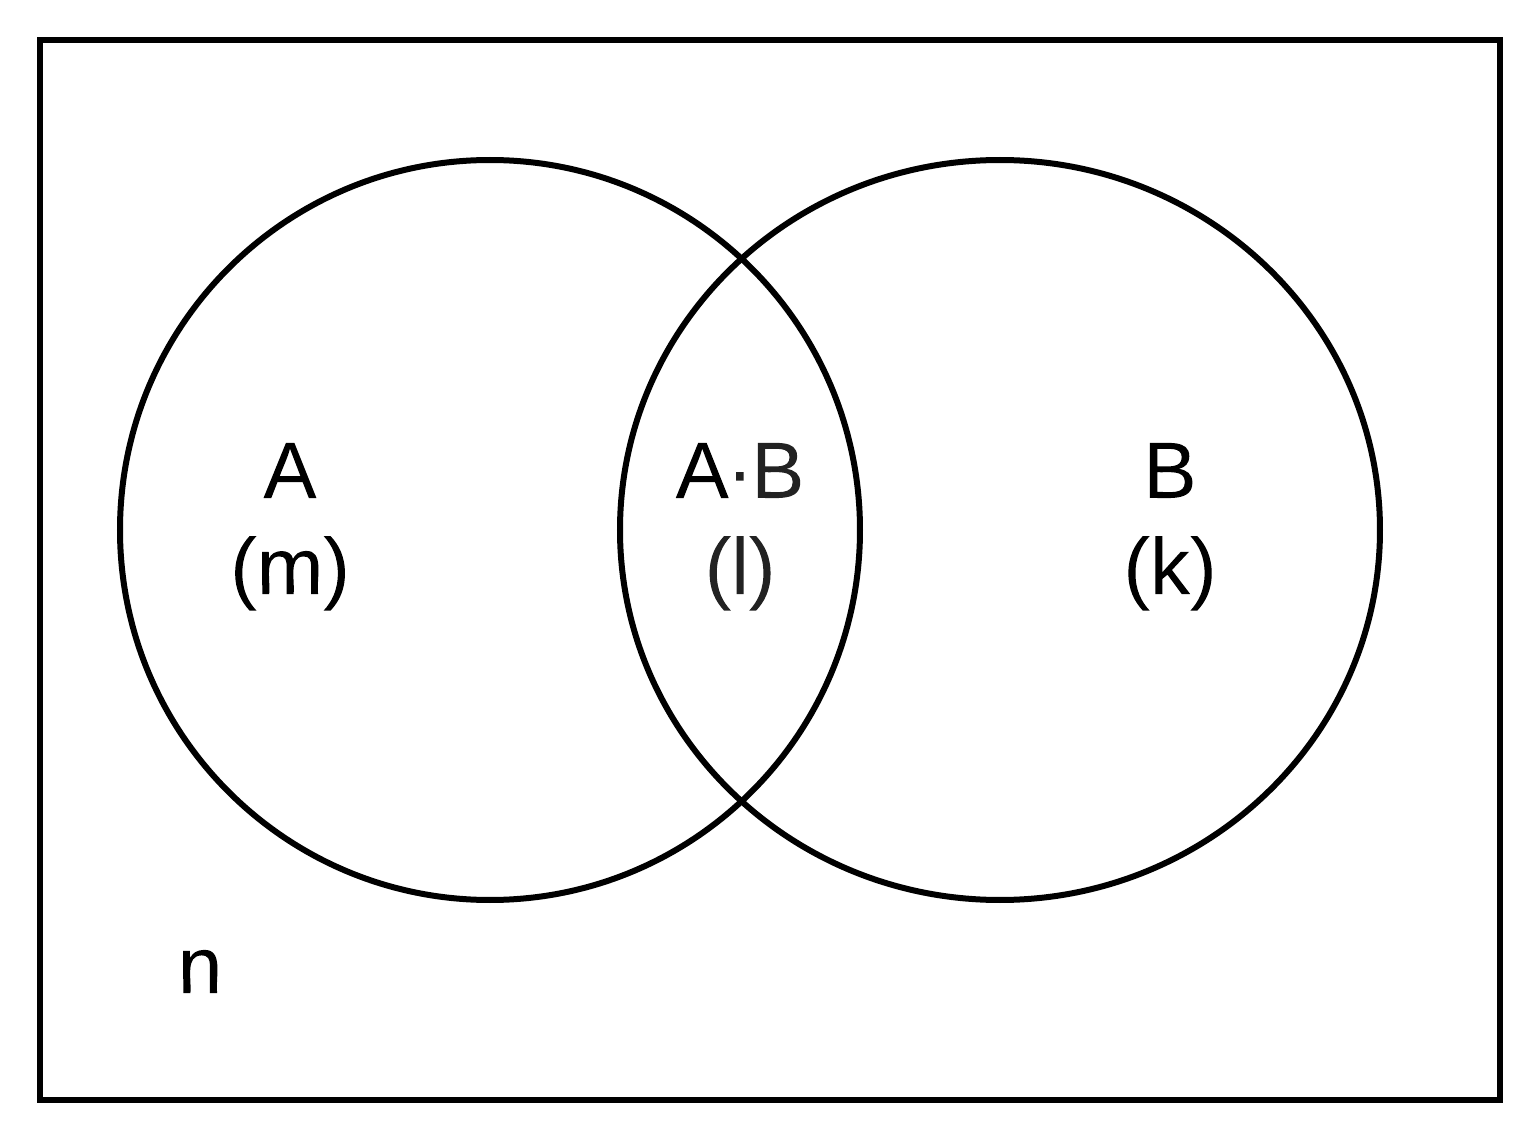
\includegraphics[scale=0.3]{Page9.png}
\caption{Произведение вероятностей}
\end{figure}\\
Для схемы случаев. Пусть в результате опыта возможно $n$ исходов, событие $A$ благоприятных $m$ исходов, событие $B$ -- $k$ исходов, и событие $A$, и событие $B$ -- $l$ исходов. $P(A\cdot B)\ =\ \frac{l}{n}$, $P(A)\ =\ \frac{m}{n}$. Если известно, что $A$ происходит, то из $n$ остальных возможных исходов, из них $l$ блокируют событие $B$, то есть  $P(A|B)=\frac{l}{m}$. То есть $P(A\cdot B) = P(A)\cdot P(B)$.\\
Ясно, что $P(A\cdot B) = P(B)\cdot P(A|B)$
\begin{flushright}\(\blacksquare\)\end{flushright}
\textbf{Следствие\ 1}\\Если событие $A$ не зависит от события $B$, то и событие $B$ не зависит от события $A$.
\begin{tabbing}
Известно, что $P(A)$ = $P(A|B)$. Считаем, что $P(A)$ $\neq$ $0$.\\
\end{tabbing}
\begin{equation*} 
 \begin{cases}
   $P(AB)$ = $P(A)P(B|A)$\\
   $P(AB)$ = $P(B)P(A|B)$
 \end{cases}
\end{equation*}
Следовательно, $P(A)P(B|A)$ = $P(B)P(A)$, следовательно\\
(при условии $P(A)$ $\neq$ $0$) $P(B|A)=P(B)$\\
То есть, свойство зависимости или независимости взаимно.\\
\textbf{Следствие\ 2}\\ Для независимых событий $P(A\cdot B)$ $=$ $P(A)\cdot P(B)$\\
\textbf{Замечание\ } \\ Эта формула может быть взята за определение независимых событий.\\
$\textbf{Теорема}$\\
Умножение для $n$ событий.\\ $P(A_1, A_2, .\ .\ .\ .\ , A_n)$=$P(A_1)\cdot P(A_2|A_1) \cdot P(A_3|A_1A_2) \ .\ .\ . \ P(A_n|A_1,A_2 .\ .\ A_n)$\\
\textit{\textbf{Определение}}\\События $A_1, A_2, .\ .\ .\ , A_n$ называются независимыми в совокупности, если :\\ $P(A_1)\cdot P(A_2) \cdot .\ .\ .\  P(A_n)$\\
\textbf{Замечание\ }  \\
Это \nolinebreak[4] определение\nolinebreak[4] эквивалентно\nolinebreak[4] следующему:  события независимы в совокупности, если любое из них не зависит любой совокупности остальных.\\
%начало страницы 10
\textbf{Замечание\ } \\ Независимость в совокупности не эквивалентна попарной независимости событий\\
\textbf{Пример\ 1 }(Пример Бернштейна): \\Имеется 4 шара. Красного, жёлтого, зелёного и трехцветный (содержащий все три цвета). (Модификация - $4$ студента, имеющие задолженности по разным предметам). Событие К --  вынули шар, на котором есть красный цвет, событие Ж -- есть жёлтый, событие З -- зелёный. $P($K$)=\frac{1}{2}$ = $P($Ж$)=P($З$)$\\
Вероятность того, что вынули шар одновременно с двумя цветами равна $P($K$\cdot$Ж$)\ =\frac{1}{4}$ = $P($К$)\cdot P($Ж$)$,  $P($K$\cdot$З$)\ =$  $P($К$)\cdot P($З$)\  = \  \frac{1}{4}$, $P($Ж$\cdot$З$)\ =$  $P($Ж$)\cdot P($З$)\  =\ \frac{1}{4}$.\\Вероятность того, что выпадет три цвета равна $P($К$\cdot$Ж$\cdot$З$)$ = $\frac{1}{4}\neq \ P($К$)\cdot P($Ж$) \cdot \cdot  P($З$)=\frac{1}{8}$ То есть они попарно независимы, но зависимы в совокупности.\\
\textbf{Пример\ 2}\\
Техническое устройство отказывает с вероятностью $p=0.5$. Сколько раз его надо продублировать, что бы вероятность отказа установки была $q < 0.1$?\\
$P=p^n<0.1=q$, $n > \frac{\ln(q)}{\ln(p)}$\\
Суммы и произведение вероятностей часто работают вместе.\\
\textbf{Пример\ 3}\\ Пусть все элементы отказывают независимо от комбинаций других. Чему равна вероятность отказа цепи?	
\begin{figure}[!h]
\begin{tikzpicture}
\draw[gray, thick] (0,7) -- (1,7);
\draw (1.5,7) circle (0.5);
\node [below] at (1.5, 6.5) {$0.1$};
\node [above] at (1.5, 7.5) {$A$};
\draw[gray, thick] (2,7) -- (3,7);
\draw[gray, thick] (3,7) -- (3,8.25);
\draw[gray, thick] (3,7) -- (3,5.75);
\draw[gray, thick] (3,8.25) -- (4,8.25);
\draw[gray, thick] (3,5.75) -- (4,5.75);
\draw (4.5,5.75) circle (0.5);
\draw (4.5,8.25) circle (0.5);
\node [below] at (4.5, 5.25) {$0.3$};
\node [above] at (4.5, 6.25) {$B_1$};
\node [below] at (4.5, 7.75) {$0.3$};
\node [above] at (4.5, 8.75) {$B_2$};

\draw[gray, thick] (5,8.25) -- (6,8.25);
\draw[gray, thick] (5,5.75) -- (6,5.75);
\draw[gray, thick] (6,5.75) -- (6,8.25);
\draw[gray, thick] (6,7) -- (7,7);

\draw[gray, thick] (7,5) -- (7,9);
\draw[gray, thick] (7,5) -- (8,5);
\draw[gray, thick] (7,9) -- (8,9);
\draw[gray, thick] (7,7) -- (8,7);
\draw (8.5,5) circle (0.5);
\draw (8.5,9) circle (0.5);
\draw (8.5,7) circle (0.5);
\node [above] at (8.5, 5.5) {$C_1$};
\node [below] at (8.5, 4.5) {$0.5$};
\node [above] at (8.5, 7.5) {$C_2$};
\node [below] at (8.5, 6.5) {$0.5$};
\node [above] at (8.5, 9.5) {$C_3$};
\node [below] at (8.5, 8.5) {$0.5$};

\draw[gray, thick] (9,5) -- (10,5);
\draw[gray, thick] (9,9) -- (10,9);
\draw[gray, thick] (9,7) -- (10,7);
\draw[gray, thick] (10,5) -- (10,9);
\draw[gray, thick] (10,7) -- (11,7);
\end{tikzpicture}
\caption{Схема цепи}
\end{figure}\\
$P(A+B_1B_2+C_1C_2C_3)=P(A)+P(B_1)\cdot P(B_2)+P(C_1C_2C_3)-P(AB_1B_2)-P(AC_1C_2C_3)-P(B_1B_2C_1C_2C_3)+P(AB_1B_2C_1C_2C_3)$\\
\begin{center}
$\textbf{Формула полной вероятности }$
\end{center}
\textit{\textbf{Определение}}\\Говорят, что события $H_1$, $H_2$, . . . $H_n$ образуют полную группу, \\если $H_1+H_2+$. . .$+H_n$ -- достоверное событие.\\
Пусть $H_1$, $H_2$, . . . $H_n$ -- полная группа попарно несовместимых событий. Эти события будем называть гипотезами. Пусть надо найти вероятность события $A$, которое может произойти вместе с одной из гипотез.\\ Тогда $P(A)=\sum\limits_{i=1}^{n}P(H_i) \cdot P(A|H_i).$(эта формула носит имя Томаса Байеса)\\
Так как $H_1$, . . .$H_n$ -- полная группа. $A$ $=$ $H_1A\ +H_2A\ +$  . . .  $+\ H_nA$.\\
 $H_1,$. . .$H_n$ -- попарно несовместные, следовательно $H_1A,$ . . . $H_nA$ -- несовместны, следовательно $P(A)=P(H_1A) +$. . . $ + P(H_nA)$ $=$ $\sum\limits_{i = 1}^{n} P(H_iA)$, следовательно, по теореме умножения $P(A)=\sum\limits_{i = 1}^{n}P(H_i)\cdot P(A|H_i)$\\
\textbf{Пример\ }\\По самолету производится 3 выстрела. Вероятность попадания при первом $0.4$, при втором -- $0.5$, при третьем -- $0.7$. Для вывода самолета из
%начало страницы 11
 строя заведомо достаточно 3 попаданий. При первом попадании самолет выходит из строя с вероятностью $0.2$, при двух -- $0.6$. Найти вероятность того, что в результате трех выстрелов самолет будет выведен из строя.\\
$H_i$ -- в самолет попал $i$--й снаряд, $P(H_0)=0.6\cdot0.5\cdot0.3=0.09$. \\
$P(H_1)=0.4\cdot0.5\cdot0.3+0.6\cdot0.5\cdot0.3+0.6\cdot0.5\cdot0.7=0.36$\\
$P(H_2)=0.6\cdot0.5\cdot 0.7+0.4\cdot0.5\cdot0.7+0.4\cdot0.5\cdot0.5=0.41$\\
$P(H_3)=0.4\cdot0.5\cdot0.7=0.14$\\
$P(A)=0.36\cdot0.2+0.41\cdot0.6+0.14\cdot1=0.458$\\
\begin{center}
$\textbf{Формула Байеса }$
\end{center}
Пусть событие $A$ может произойти с одним из $n$ попарно несовместимых событий $H_1, H_2, .\ .\ .\ H_n$, образующих полную группу. Вероятности гипотез до опыта известны -- $P(H_1)$, . . . $P(H_n)$ (априорные вероятности). Произведен опыт, в результате которого произошло событие $A$. Как следует изменить вероятности гипотез в связи с появлением $A$ (то есть найти апостериорные вероятности $P(H_i|A)$?
$P(AH_i)=P(A)\cdot P(H_i|A) = P(H_i) \cdot P(A|H_i)$, следовательно $P(H_i|A) = \frac{P(H_i) \cdot P(A|H_i)}{P(A)}$.\\
Итого: $P(H_i|A) = \frac{P(H_i)\cdot P(A|H_i)}{ \sum\limits_{j=1}^{n}P(H_j)\cdot P(A|H_j) }$\\
\\
\textbf{Пример\ }\\
В первой урне 5 белых и 10 черных шаров. Во второй -- 3 белых и 7 черных. Из второй в первую переложили $1$ шар, а затем из второй вынули один шар. Оказалось что он белый. Найти вероятность того, что был переложен белый шар\\
$H_1$ -- переложили белый, $H_2$ -- черный, $P(H_1)=\frac{3}{10}$, $P(H_2)=\frac{7}{10}$. $P(A|H_1)=\frac{6}{11}$, $P(A|H_2)=\frac{5}{11}$\\
 $P(A)=\frac{3}{10}\cdot \frac{6}{11} + \frac{7}{10} \cdot \frac{5}{11}$, $P(H_1|A)$ = $\frac {\frac{3}{10}\cdot \frac{6}{11} }   {\frac{3\cdot 6}{10\cdot11} + \frac{7\cdot5}{10\cdot11}  }$ = $\frac{18}{18 + 35}$\\
\textbf{Пример\ }\\
Известно, что $5\%$ мужчин и $0.25\%$ женщин -- дальтоники. Наугад выбранное лицо страдает дальтонизмом. Какова вероятность того, что это мужчина?\\
$P(H_1) = P(H_2) = \frac{1}{2}$\\
$P(A|H_1) = 0.05$, $P(A|H_2) = 0.0025$, $P(H_1|A) = \frac{\frac{1}{2} \cdot 0.05}{ \frac{1}{2} \cdot 0.05 + \frac{1}{2} \cdot 0.0025 } = \frac{20}{21}$\\
%начало страницы 12
\subsection{Повторение опытов}
\noindent
В самом начале развития теории вероятностей выяснилась фундаментальная роль одной математической схемы, изученной швейцарцем Якобом Бернулли.\\
Схема такая: проведем последовательность испытаний, в каждом из которых вероятность события $A$ одна и та -- же($p$). Испытания независимы, то есть вероятность выявления события $A$ в каждом из них не зависит от того, появилось оно или нет в других испытаниях.\\
\textbf{Пример\ }\\ $2$ игрока играют в шахматы $3$ партии. Вероятность выигрыша первого $p = \frac{2}{3}$. Найти вероятность того, что он выиграет $2$ партии.\\
Это можно осуществить : \\
$P(A_1A_2\overline{A_3} + A_1\overline{A_2}A_3 + \overline{A_1}A_2A_3)=\frac{2}{3}\cdot\frac{2}{3}\cdot\frac{1}{3} + \frac{2}{3}\cdot\frac{1}{3}\cdot\frac{2}{3} + \frac{1}{3}\cdot\frac{2}{3}\cdot\frac{2}{3} = \frac{4}{9}.$\\
В общем виде: вероятность $P_n(m)$  того, что в $n$ опытах событие произойдёт $m$ раз равна: $A_1A_2.\ . \ . \ A_m\overline{A_{m+1}}.\ .\ .\ \overline{A_n} + 
A_1A_2.\ . \ . \ \overline{A_m} A_{m+1} \overline{A_{m+2}} .\ .\ .\ \overline{A_n} +
\ \ \ .\ .\ .\ 
+\overline{A_1}\overline{A_2}.\ . \ . \ \overline{A_{n-m}} {A_{n-m+1}} .\ .\ .\ A_n$
В каждую комбинацию $A$ входит $m$ раз ,  $\overline{A}$ входит $n - m$ раз.
Число комбинаций $C^m_n$, все комбинации несовместны, следовательно $P_n(m) = p^mq^{n-m} + p^mq^{n-m} + .\ .\ . = C^m_np^mq^{n-m}$ , где $q = 1 - p$.\\
Так как ${P_n(m)}$ представляет из себя член разложения бинома {$(q+p)^n$}\\
 распределение вероятностей такого вида называется биноминальным распределением.\\
\textbf{Пример\ }\\
Два шахматных игрока, 10 результативных партий (ничьи не учитываются), Вероятность выигрыша первого -- $\frac{2}{3}$, второго -- $\frac{1}{3}$. Найти вероятность выигрыша
 всей игры первым?\\
$P_{выигрыша\ 1} = P_{10}(6) + P_{10}(7) + P_{10}(8) + P_{10}(9) +  P_{10}(10)$ = $\frac{2^6}{3^{10}}\cdot(210+240+180+80+16) = \frac{2^6\cdot241}{3^{9}}$
$P_{выигрыша\ 2} = P_{10}(6) + P_{10}(0) + P_{10}(1) + P_{10}(2) +  P_{10}(3)  +  P_{10}(4)$ = $\frac{1507}{3^{9}}\cdot(210+240+180+80+16)$\\
То есть вероятность выигрыша первой партии у первого в два раза больше чем у второго, вероятность выигрыша матча у первого в 10 раз больше, чем у второго.\\
\textbf{Замечание\ } \\
$\sum\limits_{m = 0}^{n}P_n(m) = 1$, $(p+q)^n=1$, $p+q = 1$, следовательно, $(p+q)^n = \sum\limits_{m = 0}^{n}P_n(m)  =\\= \sum\limits_{m = 0}^{n}C^m_np^mq^{(n-m)}$ -- Бином Ньютона.\\
%начало страницы 13
\section{Случайные величины}
\noindent
\textit{\textbf{Определение}}\\
Функция, определённая на пространстве элементарных событий называется случайной величиной.\\
\textit{\textbf{Определение}}\\
Случайная величина называется дискретной, если она определена на дискретном пространстве элементарных событий.\\
\textbf{Замечание\ } \\ Лучше бы было называть случайные величины функциями случая\\
\textbf{Пример\ }\\Дискретная случайная величина. Число тузов у одного игрока при игре в бридж, число совпадающих дней рождения в группе из $n$ человек.\\
Обозначать случайные величины будем буквами $X, Y$,... и их значения $x, y$ ...
Пусть $X$ -- случайная величина. $x_1, x_2,$ ...  --  ее значения. Совокупность всех элементарных событий, на которых $X$ принимает значение $x_i$ образует событие $X=x_i$.
Его вероятность обозначается $P(X=x_j) = p_j$. Соотношение, устанавливающее связь между значениями случайных величин и их вероятностями называется законом распределения случайной величины. Самой простой формой закона распределения для случайной величины является ряд распределения то есть таблица распределения, в которой сведены значения случайной величины и их вероятности. \\
\begin{tabular}[b]{ | l | l | l | l | }
\hline
$x_i$&$x_1$&$x_2$&$...$\\
\hline
$p_i$&$p_1$&$p_2$&$...$\\
\hline
\end{tabular}\\
Для наглядности это часто изображают на графике и точки соединяют отрезками прямых. Получившаяся фигура называется многоугольником распределения.
Так как события $X=x_j$ -- несовместимы и образуют полную группу, то $\sum\limits_{i = 1}^{n}p_i = 1$.
\begin{figure}[!h]
\begin{picture}(100,70)
\put(10, 10){\vector(0, 3){50}}
\put(10, 10){\vector(4, 0){100}}
\put(20, 15){\circle*{2}}
\put(40, 30){\circle*{2}}
\put(60, 20){\circle*{2}}
\put(20, 10){\circle*{2}}
\put(40, 10){\circle*{2}}
\put(60, 10){\circle*{2}}
\put(20, 10){\line(0, 1){5}}
\put(40, 10){\line(0, 1){20}}
\put(60, 10){\line(0, 1){10}}

\put(20, 15){\line(20, 15){20}}
\put(40, 30){\line(20,- 10){20}}

\put(20, 0){\makebox(0, 0)   {$x_1$}}
\put(40, 0){\makebox(0, 0)   {$x_2$}}
\put(60, 0){\makebox(0, 0)   {$x_3$}}
\put(110, 0){\makebox(0, 0)   {$x_i$}}
\put(0, 65){\makebox(0, 0)   {$p_i$}}

\end{picture}
\caption{Многоугольник распределения}
\end{figure}\\
\newpage
\noindent
\textbf{Пример\ }\\
Баскетболист бросает мяч в кольцо до первого попадания, либо пока не сделано 3 броска. Вероятность попадания при одном броске равна $0.7$.\\
$X$ -- число бросков.\\
\begin{tabular}[b]{ | l | l | l | l | }
\hline
$x_i$&$1$&$2$&$3$\\
\hline
$p_i$&$0.7$&$0.3\cdot0.7=0.21$&$0.3\cdot0.3 = 0.09$\\
\hline
\end{tabular}
\\
%начало страницы 14
\begin{center}
$\textbf{Функция распределения }$\\
\end{center}
Вероятность $P(X=x)$ часто использовать неудобно. Используют вероятность $P(X<x).$\\
\textit{\textbf{Определение}}\\
Функция распределения (интегральная функция распределения или интегральный закон распределения или распределение накопленой\\ вероятности)  -- это функция на вещественной оси, определяемая следующим образом: $F(x)=P(X<x)$\\
$F(x)$ полностью характеризует случайную величину с вероятностной точки зрения, то есть это форма закона распределения.\\
Свойства:\\
1)$F(x)$ -- неубывающая функция (то есть, при $x_1 < x_2$ $F(x_1) \leq F(x_2)$)\\
2)$\displaystyle{  \lim_{x\to{-\infty}}  } F(x) = 0$\\
3)$\displaystyle{  \lim_{x\to{+\infty}}  } F(x)  = 1$\\
4)$F(x)$ непрерывна слева. $\displaystyle{ F(x_i) = \lim_{x\to{x_i - 0}} F(x) }$ \\
\textit{\textbf{Определение}}\\
Случайная величина называется непрерывной, если ее функция распределения непрерывна.\\
\newpage
\begin{figure}[!h]
\begin{tikzpicture}
   \begin{axis}[ xmin=-15, xmax=15, ymin=0, ymax=2,
     ticks=none,
 axis y line=middle,
  width=6cm,height=4cm,
     axis x line=middle,
     label style={font=\normalsize},
     xlabel=$x$, ylabel=$F(x)$,
     xtick = {-10,0,...,10}, ytick = {0,...,1},
y label style={at={(axis description cs:0.21,1)},rotate=0},
     scale=1, restrict y to domain=0:10]
    \addplot[black, samples=100, smooth, unbounded coords=discard, domain=0:15] plot (\x, {1 - (1)  /( \x  + 2) }) ;
    \addplot[black, samples=100, smooth, unbounded coords=discard, domain=-15:0] plot (\x, {(1)  /( \x * (-1)  + 2) }) ;
    \draw[dashed] (axis cs: 0, 1)--(axis cs: 15,1);
 \end{axis}
\end{tikzpicture}

\caption{Непрерывная случайная величина}
\end{figure}
\noindent
Для дискретной случайной величины :$F(x) = \sum\limits_{x_j < x}P(X=x_j)$
\begin{figure}[!h]
\begin{picture}(100,100)
\put(30, 10){\vector(0, 3){80}}
\put(30, 10){\vector(4, 0){130}}
\put(20, 60){\makebox(10, 0){$1$}}
\put(10, 80){\makebox(10, 0){$F(x)$}}
\put(150, 0){\makebox(10, 0){$x$}}
\put(60, 10){\circle*{3}}
\put(80, 10){\circle*{3}}
\put(100, 10){\circle*{3}}
\put(40, 10){\circle*{3}}
\put(80, 10){\circle*{3}}
\put(30, 60){\circle*{3}}
\put(60, 20){\vector(-1, 0){20}}
\put(80, 30){\vector(-1, 0){20}}
\put(100, 40){\vector(-1, 0){20}}
\put(120, 60){\vector(-1, 0){20}}
\put(40, 10){\vector(-1, 0){10}}
\thinlines
\put(30, 10){\line(1, 0){10}}
\put(40, 0){\makebox(10, 0)   {$x_1$}}
\put(60, 0){\makebox(10, 0)   {$x_2$}}
\put(80, 0){\makebox(10, 0)   {$x_3$}}
\put(100, 0){\makebox(10, 0)   {$x_4$}}
\put(40, 10){\line(0, 1){3}}
\put(40, 16){\line(0, 1){3}}

\put(60, 10){\line(0, 1){3}}
\put(60, 16){\line(0, 1){3}}
\put(60, 22){\line(0, 1){3}}
\put(60, 28){\line(0, 1){2}}

\put(80, 10){\line(0, 1){3}}
\put(80, 16){\line(0, 1){3}}
\put(80, 22){\line(0, 1){3}}
\put(80, 28){\line(0, 1){3}}
\put(80, 34){\line(0, 1){3}}

\put(100, 10){\line(0, 1){3}}
\put(100, 16){\line(0, 1){3}}
\put(100, 22){\line(0, 1){3}}
\put(100, 28){\line(0, 1){3}}
\put(100, 34){\line(0, 1){3}}
\put(100, 40){\line(0, 1){3}}
\put(100, 46){\line(0, 1){3}}
\put(100, 52){\line(0, 1){3}}
\put(100, 58){\line(0, 1){2}}

\put(30, 60){\line(1, 0){3}}
\put(36, 60){\line(1, 0){3}}
\put(42, 60){\line(1, 0){3}}
\put(48, 60){\line(1, 0){3}}
\put(54, 60){\line(1, 0){3}}
\put(60, 60){\line(1, 0){3}}
\put(66, 60){\line(1, 0){3}}
\put(72, 60){\line(1, 0){3}}
\put(78, 60){\line(1, 0){3}}
\put(84, 60){\line(1, 0){3}}
\put(90, 60){\line(1, 0){3}}
\put(96, 60){\line(1, 0){3}}
\end{picture}
\caption{Функция распределения}
\end{figure}
\noindent
\\
\textbf{Пример\ }\\
Cо стр 11 про баскетболиста
\begin{figure}[!h]
\begin{picture}(100,100)
\put(30, 10){\vector(0, 3){80}}
\put(30, 10){\vector(4, 0){130}}
\put(20, 60){\makebox(10, 0){$1$}}
\put(10, 80){\makebox(10, 0){$F(x)$}}
\put(150, 0){\makebox(10, 0){$x$}}
\put(60, 10){\circle*{3}}
\put(80, 10){\circle*{3}}
\put(100, 10){\circle*{3}}
\put(40, 10){\circle*{3}}
\put(80, 10){\circle*{3}}
\put(30, 60){\circle*{3}}
\put(60, 20){\vector(-1, 0){20}}
\put(80, 30){\vector(-1, 0){20}}
\put(100, 40){\vector(-1, 0){20}}
\put(120, 60){\vector(-1, 0){20}}
\put(40, 10){\vector(-1, 0){10}}
\thinlines
\put(30, 10){\line(1, 0){10}}
\put(35, 0){\makebox(10, 0)   {$1$}}
\put(55, 0){\makebox(10, 0)   {$2$}}
\put(75, 0){\makebox(10, 0)   {$3$}}
\put(95, 0){\makebox(10, 0)   {$4$}}
\put(40, 10){\line(0, 1){3}}
\put(40, 16){\line(0, 1){3}}

\put(60, 10){\line(0, 1){3}}
\put(60, 16){\line(0, 1){3}}
\put(60, 22){\line(0, 1){3}}
\put(60, 28){\line(0, 1){2}}

\put(80, 10){\line(0, 1){3}}
\put(80, 16){\line(0, 1){3}}
\put(80, 22){\line(0, 1){3}}
\put(80, 28){\line(0, 1){3}}
\put(80, 34){\line(0, 1){3}}

\put(100, 10){\line(0, 1){3}}
\put(100, 16){\line(0, 1){3}}
\put(100, 22){\line(0, 1){3}}
\put(100, 28){\line(0, 1){3}}
\put(100, 34){\line(0, 1){3}}
\put(100, 40){\line(0, 1){3}}
\put(100, 46){\line(0, 1){3}}
\put(100, 52){\line(0, 1){3}}
\put(100, 58){\line(0, 1){2}}

\put(30, 60){\line(1, 0){3}}
\put(36, 60){\line(1, 0){3}}
\put(42, 60){\line(1, 0){3}}
\put(48, 60){\line(1, 0){3}}
\put(54, 60){\line(1, 0){3}}
\put(60, 60){\line(1, 0){3}}
\put(66, 60){\line(1, 0){3}}
\put(72, 60){\line(1, 0){3}}
\put(78, 60){\line(1, 0){3}}
\put(84, 60){\line(1, 0){3}}
\put(90, 60){\line(1, 0){3}}
\put(96, 60){\line(1, 0){3}}
\end{picture}
\caption{Функция распределения}
\end{figure}\\
\textbf{Пример\ }\\
Случайная величина -- площадь разрушений, наносимых цели  бомбой. Значение этой случайной величины непрерывно заполняет промежуток от $0$ $\pi R^2$ ($R$ -- радиус разрушительного действия). Но в точках $0$ и $\pi R^2$ у функции распределения скачки, так как этим значениям соотвествуют конечные вероятности (вероятности положений 1 и 3 соответственно) круга разрыва.\\
\begin{figure}[!h]
\begin{tikzpicture}
   \begin{axis}[ xmin=-18, xmax=25, ymin=0, ymax=2,
     ticks=none,
 axis y line=middle,
  width=7cm,height=4cm,
     axis x line=middle,
clip mode=individual ,
     label style={font=\normalsize},
     xlabel=$x$, ylabel=$F(x)$,
     xtick = {-10,0,...,10}, ytick = {0,...,1},
y label style={at={(axis description cs:0.23,1)},rotate=0},
     scale=1, restrict y to domain=0:10]
    \addplot[black, samples=100, smooth, unbounded coords=discard, domain=0:14.5, <-] plot (\x, {1 - (1)  /( \x  + 2) - 1/4 }) ;
    \draw[dashed] (axis cs: 0, 1)--(axis cs: 14.5,1);
 \draw[dashed] (axis cs: 14.5, 0)--(axis cs: 14.5,1);
\draw[<-](axis cs: 14.5, 1)--(axis cs: 22,1);
\draw[-, thick](axis cs: -18, 0)--(axis cs: 0,0);
   \node[label={below :{$\pi R^2$}},circle,fill,inner sep=1pt, -latex] at (axis cs:14.5,0) {};
   \node[label={ left :{$1$}},circle,fill,inner sep=1pt, -latex] at (axis cs:0,1) {};
 \end{axis}
\end{tikzpicture}
\caption{Функция распределения}
\end{figure}
\begin{figure}[!h]
\begin{tikzpicture}
\draw [pattern=north east lines] (0,0) ellipse (2cm and 1cm);
\draw [pattern=north west lines] (1,1) circle (0.5cm);
\draw [pattern=north west lines] (0.1,0.4) circle (0.5cm);
\draw [pattern=north west lines] (2,2) circle (0.5cm);
\node [black, right] at (-0.8,0.2) {$I$};
\node [black, right] at (1.4,1.3) {$II$};
\node [black, right] at (2.4,2) {$III$};
\end{tikzpicture}
\caption{Разрушения бомбой}
\end{figure}
%начало страницы 15
Вероятность попадания точки на отрезок.\\
$P(\alpha \leq  x <  \beta) = P(x < \beta) - P(x < \alpha) = F(\beta) - F(\alpha)$\\
\textbf{Замечание\ } \\
$P(\alpha \leq  x \leq  \beta) = F(\beta) - F(\alpha) + P(x = \beta)$\\
$P(x = \alpha)=$   $\displaystyle{  \lim_{\beta \to{\alpha}}} $           $ P(\alpha \leq x < \beta) =$    $\displaystyle { \lim_{\beta \to {\alpha}}} (F(\beta) - F(\alpha))$\\
Если слева величина непрерывна, то $P(x=\alpha)=0$.\\
\begin{center}
$\textbf{Плотность вероятности }$\\
\end{center}
Пусть непрерывная случайная величина имеет дифференцируемую функцию распределения. Тогда $P(x<X<x + \Delta x) =  F(x + \Delta x) - F(x)$\\
\textit{\textbf{Определение}}\\ $f(x) =$ $\displaystyle { \lim_{{\Delta x} \to {0}}}$ $\frac{P(x<X<x+\Delta x)}{\Delta x}$ = $F'(x)$ -- плотность вероятности (плотность распределения).\\
$F(x)$ -- первообразная для $f(x)$. Так как $F(-\infty)=0$, то константа в первообразной выбирается однозначно.\\
$F(x) = \int\limits_{-\infty}^{x}f(x)dx$\\
Найдем $P(\alpha < X < \beta)$ через $f(x)$. Так как вероятность одного значения непрерывной случайной величины равна нулю: $P(\alpha <  X < \beta) = \\=P(\alpha \leq  X < \beta) = F(\beta) - F(\alpha)=  \int\limits_{-\infty}^{\beta}f(x)dx -   \int\limits_{-\infty}^{\alpha}f(x)dx =  \int\limits_{\alpha}^{\beta}f(x)dx$.
\begin{figure}[!h]
\begin{tikzpicture}
   \begin{axis}[ xmin=-2, xmax=2, ymin=-2, ymax=8,
     ticks=none,
     axis y line=middle,
     axis x line=middle,
     y label style={at={(axis description cs:.55,0.9)},anchor=south },
%y label style={ticks=none,at={(axis description cs:0.2,10)},rotate=270,anchor=south},
     axis line style={->},
     xlabel=$x$, ylabel=$f(x)$,
     scale=1]
     %\addplot[domain=-pi/2:pi/2,samples=200,black,pattern=north east lines]{cos(deg(x)) + sin(deg(x)) + 3};
     %\addplot[domain=-pi/2:pi/2,samples=200,black]{cos(deg(x))};
     \node[label={below :{$\alpha$}},circle,fill,inner sep=1pt] at (axis cs:-pi/2 + 0.30,0) {};
     \node[label={below:{$\beta$}},circle,fill,inner sep=1pt] at (axis cs:pi/2 - 0.30,0) {};
     \addplot[domain=-pi/2 + 0.3:pi/2 - 0.3,samples=200,black,pattern=north east lines]{cos(deg(x)) + sin(deg(x)) + 3}\closedcycle;	
     \addplot[domain=-pi/2:pi/2,samples=200]{cos(deg(x)) + sin(deg(x)) + 3};
     
\end{axis}
\end{tikzpicture}
\caption{График функции распределения}
\end{figure}\\
Геометрически $P(\alpha<x<\beta)$ -- это площадь.\\
%начало страницы 16
Свойства плотности вероятности:\\
1)$f(x)\geqslant 0$ (следует из того, что $F(x)$ неубывает)\\
2)$  \int\limits_{-\infty}^{\infty}f(x)dx=1$(так как $F(\infty) = 1$)\\
То есть график плотности вероятности выше оси абсцисс, а полная площадь равна 1.\\
\textbf{Пример\ }\\
\begin{equation*} 
f(x)=
 \begin{cases}
   a \cdot \cos(x), -\frac{\pi}{2} \leq x \leq \frac{\pi}{2} \\
   0 , x < -\frac{\pi}{2} $ или $ x > \frac{\pi}{2}
 \end{cases}
\end{equation*}
\begin{figure}[!h]
\begin{tikzpicture}
   \begin{axis}[ xmin=-2.0, xmax=2.0, ymin=0, ymax=1 ,
     ticks=none,
     axis y line=middle,
     axis x line=middle,
width=6cm,
  height=4cm,
clip mode=individual ,
     y label style={at={(axis description cs:.6,0.8)},anchor=south },
     x label style={at={(axis description cs:1,0)}},
%y label style={ticks=none,at={(axis description cs:0.2,10)},rotate=270,anchor=south},
     axis line style={->},
     xlabel=$x$, ylabel=$f(x)$,
     scale=1]
     \addplot[domain=-pi/2:*pi/2,samples=200,black]{cos(deg(x))/2};
     \node[label={below :{$\frac{\pi}{2}$}},circle,fill,inner sep=1pt, -latex] at (axis cs:-pi/2,0) {};
     \node[label={below:{$-\frac{\pi}{2}$}},circle,fill,inner sep=1pt, -latex] at (axis cs:pi/2,0) {};
     \node[label={above left:{a}},circle,fill,inner sep=1pt] at (axis cs:0,0.5) {};
\end{axis}
\end{tikzpicture}
\caption{График $f(x)$}
\end{figure}\\

$  \int\limits_{-\frac{\pi}{2}}^{\frac{\pi}{2}}a\cdot \cos x dx = 2a = 1$, следовательно, $a = \frac{1}{2}$\\
\begin{equation*} 
F(x)=
 \begin{cases}
   0 , x < -\frac{\pi}{2}\\
   \frac{1}{2} \cdot (sin(x) + 1) , \frac{\pi}{2} \leq x \leq \frac{\pi}{2} \\
   1 ,  x > \frac{\pi}{2}
 \end{cases}
\end{equation*}

\begin{figure}[!h]
\begin{tikzpicture}
   \begin{axis}[ xmin=-2, xmax=2, ymin=0, ymax=2,
     ticks=none,
     axis y line=middle,
     axis x line=middle,
width=6cm,
  height=4cm,
clip mode=individual ,
     y label style={at={(axis description cs:.6,0.85)},anchor=south },
%y label style={ticks=none,at={(axis description cs:0.2,10)},rotate=270,anchor=south},
     axis line style={->},
     xlabel=$x$, ylabel=$F(x)$,
     scale=1]
     \addplot[domain=-pi/2:pi/2,samples=200,black]{1/2*(1+sin(deg(x)))};
     \addplot[domain=pi/2:3,samples=200,black]{1};
     \node[label={below :{$\frac{\pi}{2}$}},circle,fill,inner sep=1pt] at (axis cs:-pi/2,0) {};
     \node[label={below:{$-\frac{\pi}{2}$}},circle,fill,inner sep=1pt] at (axis cs:pi/2,0) {};
     \node[label={above left:{a}},circle,fill,inner sep=1pt] at (axis cs:0,1) {};
\end{axis}
\end{tikzpicture}
\caption{График $F(x)$}
\end{figure}
%начало страницы 17
\begin{center}
$\textbf{Числовые характеристики случайных величин. }$\\
\end{center}
Функция распределения или плотность полностью описывает случайную величину с вероятностной точки зрения.\\
\begin{tabular}[b]{ | l | l | l | }
\hline
Характеристика &  Дискретная & Непрерывная   \\
 &  случайная  & случайная  \\
 &  величина X  & величина X  \\
\hline
Математическое ожидание &  $ \sum\limits_{k} x_kp_k$ & $\int\limits_{-\infty}^{\infty}xf(x)dx$\\
Дисперсия & $\sum\limits_{k}^{}(x_k-M(x))^2p_k$ & $\int\limits_{-\infty}^{\infty}(x- M(x))^2f(x)dx$\\
Начальный момент & $\sum\limits_{k} x^s_kp_k$ & $\int\limits_{-\infty}^{\infty}x^sf(x)dx$\\
порядка S& &\\
Центральный момент& $\sum\limits_{k}^{}(x_k-M(x))^sp_k$& $\int\limits_{-\infty}^{\infty}(x- M(x))^sf(x)dx$\\
порядка S& &\\
Мода&наиболее вероятное&значение, \\
& значение& в котором f(x)\\
& &максимально\\
Медиана&не определяем -- &такое $X$= $Me$, что \\
&редко используется&$P(X < Me)=$\\
&(такое значение $x_k,$ что &  $=P(X > Me)$\\
& $p_1+ ...+p_{k - 1} \leq \frac{1}{2}$ и&\\
& $p_1+ ...+p_{k} > \frac{1}{2})$ & \\
Среднеквадратичное  & $\sigma(x) = \sqrt{D(x)}$ & $\sigma(x) = \sqrt{D(x)}$\\
отклонение $\sigma(x)$ & &\\
Коэффициент симметрии $S_k$ & $S_k$ = $\frac{\mu_3}{\sigma^3}$ &  $S_k$ = $\frac{\mu_3}{\sigma^3}$ \\
Эксцесс $E_x$ & $E_x$ = $\frac{\mu_4}{\sigma^4}$ & $E_x$ = $\frac{\mu_4}{\sigma^4} - 3$\\
\hline
\end{tabular}\\
\textit{\textbf{Определение}}\\
Математическое ожидание дискретной случайной величины (среднее значение) -- это число $M(X)(E(X), \overline{X} , <X>)$, определяется по формуле $M(X)=\sum\limits_{k}x_kp_k$, при условии, что ряд абсолютно сходится. Если ряд абсолютно расходится, то говорят что $X$ не имеет конечного математического ожидания. Пусть случайная величина может принимать одно из $N$ равновероятных \\ значений $x_1,x_2,$ . . .$x_n$. Тогда $p_i = \frac{1}{N}$ и $M(X) = \frac{\sum\limits_{i = 1}^{N}  x_i } { N }$ -- среднее арифметическое. Если значение не является равновероятным, то надо брать взвешенное среднее, что и сделано в определении. Аналогично с точечными массами и центром масс.\\
\textbf{Замечание\ } \\
$M(X)$ может не быть значением случайной величины.\\
\textbf{Пример\ }\\
Испытываются однотипные приборы. Вероятность каждого пройти испытание равно p и независимы. Испытания заканчиваются после выхода из строя первого же прибора. $X$ -- число произведенных испытаний. Чему равно $M(X)$?\\
$P(X=k) = q\cdot p ^{k - 1}$, $q = 1 - p$.\\
\begin{tabular}[b]{ | l | l | l | l | l |   }
\hline
$x_i$&$1$&$2$&$3$&$...$\\
\hline
$p_i$&$q$&$qp$&$qp^2$&...\\
\hline
\end{tabular}\\
$M(X) = 1\cdot q + 2q\cdot p + 3 q \cdot p^2 + .\ .\ .\ +k\cdot q\cdot p^{k-1}$ = $q(1+2p+3p^2 + \ .\ .\ )'$ = $q\cdot(\frac{p}{1-p}) ' = \frac{q}{{(1-p)}^2} = \frac{1}{q}$\\
%начало страницы 18
\textbf{Пример\ }\\
 Пример отсутствия конечного математического ожидания -- "Петербургская игра". Бросается монета до тех пор, пока не выпадет орёл. Если это случается при бросании c номером $r$, то игрок получит $2^r$ рублей. $x_r=2^r$, $p_r=2^{-r}$.\\ $\sum\limits_{r = 1}^{\infty}  x_rp_r = \sum\limits_{r = 1}^{\infty} 1 = \infty$\\
\textit{\textbf{Определение}}\\
Мода -- координата максимума $f(x)$. Если кривая распределения имеет более одного максимума, то распределение называется полимодальным.
\begin{figure}[!h]
\resizebox{180pt}{140pt}{
\begin{tikzpicture}
   \begin{axis}[xmin=-5, xmax=5, ymin=0, ymax=0.4,
      axis y line=middle,
     axis x line=middle,
    ticks=none,
     xlabel=$x$, ylabel=$f(x)$,
     label style={font=\normalsize},
y label style={at={(axis description cs:0.35,1)},rotate=0},
x label style={at={(axis description cs:1,0.05)}},
    xtick = {-10,0,...,10}, ytick = {0,...,1},
    at={(0.04\linewidth,0.06\linewidth)},
     scale=1, restrict y to domain=0:5]
     \addplot[black, samples=100, smooth, unbounded coords=discard] plot (\x, { (1/  (sqrt(2*3.14)) * pow(2.17, (-1.2*(\x-0.37)*1.2*(\x - 0.37)/4)  )  / 3  });
     \draw[dashed] (axis cs: 0.37, 0)--(axis cs: 0.37,0.133014);
   \end{axis}
 \node[label={below right :{$M$}},circle,fill,inner sep=1pt] at (4.265,0.06\linewidth) {};
\end{tikzpicture}
}
\caption{Мода $f(x)$}
\end{figure}\\
\textit{\textbf{Определение}}\\	
Медиана -- $P(X<Me) = P(X>Me)$, для непрерывной случайной величины.\\
\begin{figure}[H]
\begin{tikzpicture}
   \begin{axis}[ xmin=-3, xmax=9, ymin=0, ymax=0.7,
     ticks=none,
 axis y line=middle,
clip mode = individual,
     axis x line=middle,
  width=6cm,height=5cm,
     label style={font=\normalsize},
     xlabel=$x$, ylabel=$f(x)$,
     xtick = {-10,0,...,10}, ytick = {0,...,1},
y label style={at={(axis description cs:0.25,1)},rotate=0},
     scale=1, restrict y to domain=0:10]
    \addplot[black, samples=100, smooth, unbounded coords=discard, domain=-3:2.5, pattern=north east lines] plot (\x, { (pow(2.17, (-\x + 2)/2) * (pow(2.17, (-\x + 2)/2  ) )* pow(2.17, pow(pow(2.17, (-\x + 2)/2), 2) * (-1) ) })\closedcycle;	
    \addplot[black, samples=100, smooth, unbounded coords=discard, domain=2.5:9, ,pattern=north west lines] plot (\x, { (pow(2.17, (-\x + 2)/2) * (pow(2.17, (-\x + 2)/2  ) )* pow(2.17, pow(pow(2.17, (-\x + 2)/2), 2) * (-1) ) }) \closedcycle;	
\draw[dashed] (axis cs: 2.5, 0)--(axis cs:2.5,0.4);
     \node [black, below, -latex] at (axis cs: 2.5, 0) {$Me$};
 \end{axis}
\end{tikzpicture}
\caption{Медиана случаной величины}
\end{figure}

\begin{figure}[H]
\begin{tikzpicture}
   \begin{axis}[ xmin=-21, xmax=10, ymin=0, ymax=0.7,
     ticks=none,
 axis y line=middle,
     axis x line=middle,
  width=6cm,height=5cm,
     label style={font=\normalsize},
     xlabel=$x$, ylabel=$f(x)$,
     xtick = {-10,0,...,10}, ytick = {0,...,1},
y label style={at={(axis description cs:0.65,1)},rotate=0},
 x label style={at={(axis description cs:1.1,0)}},
     scale=1, restrict y to domain=0:10]
    \addplot[black, samples=100, smooth, unbounded coords=discard, domain=-3:9] plot (\x, { (pow(2.17, (\x - 5)/2) * (pow(2.17, (\x - 5)/2  ) )* pow(2.17, pow(pow(2.17, (\x - 5)/2), 2) * (-1) ) }) ;
   \addplot[black, samples=100, smooth, unbounded coords=discard, domain=-23:-3] plot (\x, { (pow(2.17, (-\x - 13)/2) * (pow(2.17, (-\x - 13)/2  ) )* pow(2.17, pow(pow(2.17, (-\x - 13)/2), 2) * (-1) ) }) ;

 

 \end{axis}
\end{tikzpicture}
\caption{Полимодальное распределение}
\end{figure}
\noindent
\textit{\textbf{Определение}}\\
Квантиль порядка $p$ -- это значение $x_p$, соответствующее значению функции распределения равному $p$ $(F(xp)=p)$. Медиана -- квантиль порядка $\frac{1}{2}$.\\
\textit{\textbf{Определение}}\\
Центрированной случайной величиной $X$,cоответствующей величине $X$\\ называется отклонение случайной величины $X$ ее математического\\ ожидания($A$). Как оценить разброс $X$ относительно среднего?\\
 Можно рассмотреть $M(A)$, но он оказывается равен 0.\\
$M(X - m_x) = \sum\limits_{i=1}^{n}(x_i-m_x)p_i=\sum\limits_{i=1}^{n}x_ip_i - m_x\sum\limits_{i=1}^{n}p_i = m_x - m_x = 0$\\
Поэтому используют $M((X-m_x)^2)$ = $D(X)$ = $Var(X)$\\
$D(X)= \sum\limits_{i=1}^{n} (x_i - m_x)^2p_i$ = $\sum\limits_{i=1}^{n}x_i^2 - 2m_x\sum\limits_{i=1}^{n}x_ip_i + m_x^2\sum\limits_{i=1}^{n}p_i = \sum\limits_{i=1}^{n}x_i^2p_i - m_x^2$\\
Для непрерывных величин: $D(X) = \int\limits_{-\infty}^{\infty}x^2f(x)dx - m_x^2$\\
Разброс характеризуется средним квадратичным отклонением: $\sigma(x) = \sqrt{D(x)}$\\
\textbf{Пример\ }\\
\begin{equation} 
f(x)=
 \begin{cases}
   2x,  x \in [0, 1]\\
   0 , x \notin [0, 1]\\
 \end{cases}
\end{equation}
 \begin{figure}[!h]
\begin{tikzpicture}
   \begin{axis}[ xmin=-2, xmax=2, ymin=-0.5, ymax=1.5,
     ticks=none,
     axis y line=middle,
     axis x line=middle,
     label style={font=\normalsize},
     y label style={at={(axis description cs:.6,0.9)},anchor=south },
%y label style={ticks=none,at={(axis description cs:0.2,10)},rotate=270,anchor=south},
     axis line style={->},
     xlabel=$x$, ylabel=$F(x)$,
     scale=1]
     \addplot[domain=-4:0	,samples=200,black]{0};
     \addplot[domain=0:1,samples=200,black]{x};
     \addplot[domain=1:4,samples=200,black]{0};
     \node[label={below  :{$1$}},circle,fill,inner sep=1pt] at (axis cs:1,0) {};
     \node[label={below left:{$0$}},circle,fill,inner sep=1pt] at (axis cs:0,0) {};
     \node[label={below :{$\frac{1}{\sqrt{2}}$}},circle,fill,inner sep=1pt] at (axis cs:0.701,0) {};
     \draw[dashed] (axis cs: 0.701, 0)--(axis cs: 0.701,0.701);
     \draw[dashed] (axis cs: 1, 0)--(axis cs: 1,1);
\end{axis}
\end{tikzpicture}
\caption{График $f(x)$}
\end{figure}\\
$M(X) = \int\limits_{0}^{1}x\cdot 2x d x  = \frac{2}{3}$\\
$D(x) = \int\limits_{0}^{1}x^2\cdot 2x d x - \frac{4}{9} = \frac{1}{2} - \frac{4}{9} = \frac{1}{18}$\\
$\sigma(x) = \frac{1}{3\sqrt{2}}$
Чему равно $x_p$?\\
$F(x) = \int\limits_{0}^{\infty}2tdt = x^2$, $x^2 = p$, следовательно, $x_p = \sqrt{p};\\
 M_e = x_\frac{1}{2} = \frac{1}{\sqrt{2}}$\\
%страница 19
Начальный момент порядка S: $\alpha_S$ = $\sum\limits_{k} x^s_kp_k$  = $\int\limits_{-\infty}^{\infty}x^sf(x)dx$\\
Центральный момент порядка S:  $\mu_2 = \sum\limits_{k}^{}(x_k-M(x))^sp_k$  = $\int\limits_{-\infty}^{\infty}(x- M(x))^sf(x)dx$\\
Центральный и начальный моменты связаны: $\mu_2 = \alpha_2 - m_x^2$\\
$\mu_3 = \sum\limits_{i}^{n}(x_i-m_x)^3p_i =\sum\limits_{i}^{}x_i^3p_i - 3m_x\sum\limits_{i}^{ }x_i^2p_i + 3m_x^2\sum\limits_{i}^{ }x_ip_i - m_x^3\sum\limits_{i}^{ }p_i = \\
= \alpha_3 - 3 m_x \alpha_2  + 2m_x^3$\\
Можно определить моменты не относительно $m_x$, а относительно точки $a$:\\ $M((x-a)^s)$.\\
Однако центрированные имеют преимущество.
\\В  частности :$D(X) = $min$ M((x-a)^2)$\\
\underline{Доказательство:}\\
$M(X-a)^2$ = $\int\limits_{-\infty}^{\infty}(x-m_x+m_x-a)^2f(x)dx$ = $\int\limits_{-\infty}^{\infty}(x-m_x)^2f(x)dx + 2(m_x-a)\cdot \\
 \cdot \int\limits_{-\infty}^{\infty}(x-m_x)f(x)dx + (m_x - a)^2 \int\limits_{-\infty}^{\infty} f(x)dx = D(X) + (m_x-a)^2$,\\ следовательно минимум достигается при $m_x=a$
\begin{flushright}\(\blacksquare\)\end{flushright}
Нечетные центральные моменты характеризуют симметрию распределения (кроме первого, который всегда ноль). Поэтому для характеристики симметрии выбирают третий центральный  момент.
Коэфициент симметрии: $S_k(x) = \frac{\mu_3}{\sigma^3}$.\\
Если симметрия относительно $m_x$, то $S_k = 0$.\\
Четвертый момент служит для характеристики крутости, то есть\\
 островершинности или плосковершинности распределения. За стандартное распределение,  с которым проводится сравнение принято нормальное распределение: $f(x) = \frac{1}{\sqrt{2\pi}\sigma}\cdot e^{-\frac{(x-m_x)^2}{2\sigma^2}}$. \\
Его эксцесс = $E_x = \frac{\mu_4}{\sigma_4} - 3$. Для нормального $E_x = 0$.
\begin{figure}[H]
\begin{tikzpicture}
   \begin{axis}[ xmin=-3, xmax=12, ymin=0, ymax=0.8,
     ticks=none,
 axis y line=middle,
     axis x line=middle,
  width=5cm,height=5cm,
     label style={font=\normalsize},
     xlabel=$x$, ylabel=$f(x)$,
     xtick = {-10,0,...,10}, ytick = {0,...,1},
y label style={at={(axis description cs:0.20,1)},rotate=0},
     scale=1, restrict y to domain=0:10]
    \addplot[black, samples=100, smooth, unbounded coords=discard, domain=-10:10] plot (\x, { (1/  (sqrt(2*3.14) * 2) * pow(2.17, (-(\x-3)*(\x-3)/(2*4))  )  }) ;
    \addplot[black, samples=100, smooth, unbounded coords=discard, domain=-10:10] plot (\x, { (1/  (sqrt(2*3.14) * 4) * pow(2.17, (-(\x-3)*(\x-3)/16)  )  });
     \addplot[black, samples=100, smooth, unbounded coords=discard, domain=-10:10] plot (\x, { (1/  (sqrt(2*3.14)) * pow(2.17, (-(\x-3)*(\x-3)/2)  )  });	  
     \node [black, right] at (axis cs: 6, 0.43) {$E_x > 0$};
    \draw[->](axis cs:6.2, 0.43) -- (axis cs:3.1, 0.42);
    \draw[->](axis cs:6.2, 0.33) -- (axis cs:3.1, 0.21);
    \draw[->](axis cs:6.2, 0.22) -- (axis cs:3.1, 0.11);
     \node [black, right] at (axis cs: 6, 0.33) {$E_x = 0$};
     \node [black, right] at (axis cs: 6, 0.22) {$E_x < 0$};
 \end{axis}
\end{tikzpicture}
\caption{   Распределения с различными эксцессами}
\end{figure}
\begin{figure}[H]
\begin{tikzpicture}
   \begin{axis}[ xmin=-3, xmax=9, ymin=0, ymax=0.7,
     ticks=none,
 axis y line=middle,
     axis x line=middle,
  width=6cm,height=5cm,
     label style={font=\normalsize},
     xlabel=$x$, ylabel=$f(x)$,
     xtick = {-10,0,...,10}, ytick = {0,...,1},
y label style={at={(axis description cs:0.25,1)},rotate=0},
     scale=1, restrict y to domain=0:10]
    \addplot[black, samples=100, smooth, unbounded coords=discard, domain=-3:9] plot (\x, { (pow(2.17, (-\x + 2)/2) * (pow(2.17, (-\x + 2)/2  ) )* pow(2.17, pow(pow(2.17, (-\x + 2)/2), 2) * (-1) ) }) ;
\draw[dashed] (axis cs: 2.5, 0)--(axis cs:2.5,0.4);
     \node [black, right] at (axis cs: 5, 0.4) {$S_k > 0$};

 \end{axis}
\end{tikzpicture}
\caption{Коэффициент симметрии больше нуля}
\end{figure}
\begin{figure}[H]
\begin{tikzpicture}
   \begin{axis}[ xmin=-3, xmax=9, ymin=0, ymax=0.7,
     ticks=none,
 axis y line=middle,
     axis x line=middle,
  width=6cm,height=5cm,
     label style={font=\normalsize},
     xlabel=$x$, ylabel=$f(x)$,
     xtick = {-10,0,...,10}, ytick = {0,...,1},
y label style={at={(axis description cs:0.25,1)},rotate=0},
     scale=1, restrict y to domain=0:10]
    \addplot[black, samples=100, smooth, unbounded coords=discard, domain=-3:9] plot (\x, { (pow(2.17, (\x - 5)/2) * (pow(2.17, (\x - 5)/2  ) )* pow(2.17, pow(pow(2.17, (\x - 5)/2), 2) * (-1) ) }) ;
\draw[dashed] (axis cs: 4.57, 0)--(axis cs:4.57,0.4);
   \node [black, right] at (axis cs: 0.1, 0.4) {$S_k < 0$};

 \end{axis}
\end{tikzpicture}
\caption{Коэффициент симметрии меньше нуля}
\end{figure}
\noindent
\textbf{Пример\ }\\
\begin{equation*} 
f(x)=
 \begin{cases}
   2x,  x \in [0, 1]\\
   0 , x \notin [0, 1]\\
 \end{cases}
\end{equation*}\\
$\alpha_3 = 2\int\limits_{0}^{1}x^4dx=\frac{2}{5}$, $\mu_3 = \alpha_3 - 3m_x\alpha_2 + 2m_x^3 = \frac{2}{5} - 3\cdot\frac{2}{3}\cdot\frac{1}{2} + 2 \cdot (\frac{2}{3})^3 = \frac{1}{135}$\\
$S_k = \frac{\mu_3}{\sigma_3} = -\frac{2}{5}\sqrt2$\\
$\mu_4 = 2\int\limits_0^1x^4dx=2\int\limits_0 ^1(x-\frac{2}{3})^5dx + \frac{4}{3}\int\limits_{0}^{1}(x-\frac{2}{3})^4dx$ = $\frac{1}{3^7} - \frac{2^6}{3^7} + \frac{4}{15} \cdot \frac{4^0}{3^5} + \frac{2^7}{5\cdot3^6}$ = $\frac{2^2}{3^3} - \frac{2^8}{3^3} + \frac{16}{5\cdot3^2} + \frac{2^9}{5\cdot3^2}$ $>0$.\\
%страница 20
Помимо важных отдельных моментов существенных значений имеет полный набор моментов ($\mu_n$ или $\alpha_n$). Часто проще найти полный набор %хз
, чем само распределение. А при весьма общих условиях набор моментов полностью определяет распределение вероятности.\\
$\textbf{Теорема}$\\
Если две плотности вероятности $f_1(x)$ и $f_2(x)$ -- непрерывные случайные величины имеют одинаковые моменты $\alpha$ и функция $f_1(x) - f_2(x)$ представляется сходящимся на $(-\infty;\infty)$ рядом по степеням $x$, то $f_1(x) = f_2(x)$.\\
\underline{Доказательство:}\\
Пусть $f_1(x) - f_2(x)= c_0 + c_1x + c_2x^2 +$ . . . =\\
$=\int\limits_{-\infty}^{\infty} (f_1(x) - f_2(x))^2dx = \int\limits_{-\infty}^{\infty} (f_1(x) - f_2(x))(c_0 + c_1x + c_2x^2 + .\ .\ .\ .)dx=$\\
$=c_0\int\limits_{-\infty}^{\infty}(f_1(x)-f_2(x))dx + c_1\int\limits_{-\infty}^{\infty}(xf_1(x) - xf_2(x))dx +\\ +   c_2\int\limits_{-\infty}^{\infty}(x^2f_1(x) - x^2f_2(x))dx  + \ . \ .\ .\ = $\\
$=c_0(1 - 1) + c_1(\alpha_1-\alpha_1) + c_2(\alpha_2 - \alpha_2) + $ . . . $=0$, следовательно, $f_1(x) = f_2(x)$.
\begin{flushright}\(\blacksquare\)\end{flushright}
\textbf{Замечание\ } \\ 
Для "смешанной"\  случайной величины формулы дискретной и непрерывной объединяются для значений $0\leq x< 1$ -- плотность $f(x) = \frac{1}{2}$.\\
$M(X) = 0\cdot \frac{3}{8} + 1\cdot \frac{1}{8} + \int\limits_{0}^{1}x\cdot \frac{1}{2} dx = \frac{3}{8}$
%страница 21
\section{Различные законы распределения величин}
\subsection{Равномерные распределения}
\noindent
Равномерно распределённая непрерывная случайная величина -- случайная величина, у которой плотность вероятности постоянна на некотором интервале, а вне него равна нулю.\\
\textbf{Пример\ }\\
Колесо рулетки. Зафиксируем некоторое направление. Тогда угол под которым она останавливается -- случайная величина, равномерно распределённая в интервале $(0, 2\pi)$.\\
\textbf{Пример\ }\\
Производится взвешивание на весах с ценой деления 1 грамм. Если оказывается что вес заключен от $k$ до $k + 1$ грамм, тогда его можно принять за $(k + \frac{1}{2})$ и считать, что при этом допущена ошибка $X$ -- случайная величина, равномерно распределённая на интервале $(-\frac{1}{2}, \frac{1}{2})$ грамм.\\
%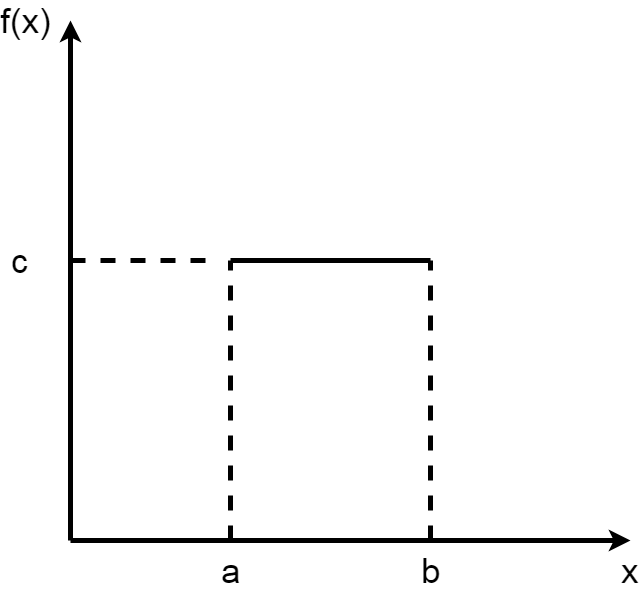
\includegraphics[scale=0.2]{Gr.png}\\
\begin{figure}[!h]	
\begin{tikzpicture}
\begin{scope}
  \begin{axis}[ ticks=none,xmin=0, xmax=2, ymin=0, ymax=1,
     y label style={at={(axis description cs:-0.3,1)},rotate=270,anchor=south},
     axis x line=middle,
     axis y line=middle,
     label style={font=\normalsize},
     xlabel=$x$, ylabel=$f(x)$,
     yticklabels=\empty,
     xticklabels=\empty,
     at={(0.001\linewidth,0.001\linewidth)},
     width=5cm,height=5cm,
     scale=1]
     \draw[ultra thick] (50,50) --(100,50);
     \draw[dashed] (0, 50) -- (50, 50);
     \draw[dashed] (50, 0) -- (50, 50);
     \draw[dashed] (100, 0) -- (100, 50);
     \node [black, right] at (28,5) {$a$};
     \node [black, right] at (-4, 55) {$c$};
     \node [black, right] at (78,5) {$b$};
\end{axis}
     \draw[fill=black!10!black] (0,1.6895) circle (0.2ex);
     \draw[fill=black!10!black] (0.875,0) circle (0.2ex);
     \draw[fill=black!10!black] (1.750,0) circle (0.2ex);    
 \end{scope}
\end{tikzpicture}
\caption{График функции распределения $f(x)$}
\end{figure}\\
Пусть распределение $X$ равномерно на $(a, b)$.\\
\begin{equation*} 
f(x)=
 \begin{cases}
   c,   x \in [a, b]\\
   0 , x \notin [a, b]\\
 \end{cases}
\end{equation*}\\
$\int\limits_{a}^{b} c dx = c(b - a)$ = 1, значит $c = \frac{1}{b - a}$\\
Итого, \\
\begin{equation*} 
f(x)=
 \begin{cases}
   \frac{1}{b - a},   x \in [a, b]\\
   0 , x \notin [a, b]\\
 \end{cases}
\end{equation*}\\
Значит, \\
\begin{equation*} 
f(x)=
 \begin{cases}
   c,   x \in [a, b]\\
   0 , x \notin [a, b]\\
 \end{cases}
\end{equation*}\\
Итого, \begin{equation*} 
F(x)=
 \begin{cases}
    0,   x \leq a\\
   \frac{x - a}{x - b} , a < x < b\\
   1, x \geq b\\
\end{cases}
\end{equation*}\\
%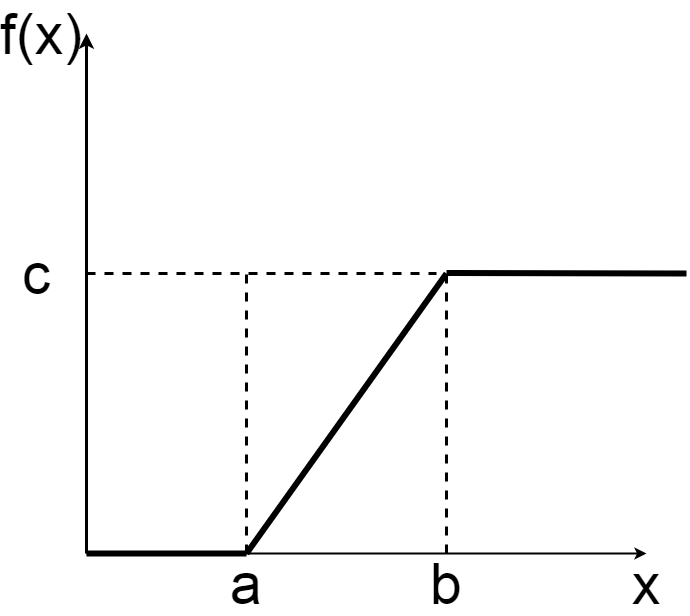
\includegraphics[scale=0.2]{Gr2.png}\\	
\begin{figure}[!h]
\begin{tikzpicture}
   \begin{axis}[ ticks=none,xmin=0, xmax=2, ymin=0, ymax=1,
     y label style={at={(axis description cs:0.1,1)},rotate=270,anchor=south},
     axis x line=middle,
     axis y line=middle,
     width=5cm,height=5cm,
     label style={font=\normalsize},
     xlabel=$x$, ylabel=$F(x)$,
     yticklabels=\empty,
     xticklabels=\empty,
     at={(0.001\linewidth,0.001\linewidth)},
     scale=1]
\draw[ultra thick] (0,0) --(50,0);
\draw[ultra thick] (50,0) --(100,50);
\draw[ultra thick] (100,50) --(150,50);
\node(3,3)  [below] {1};	
\node [black, right] at (27,7) {$a$};
\node [black, right] at (100,8) {$b$};
\node [black, right] at (0,43) {$c$};
 \draw[dashed] (0, 50) -- (100, 50);
 \draw[dashed] (50, 0) -- (50, 50);
 \draw[dashed] (100, 0) -- (100, 50);
  %   \draw[dashed] (86, 0) -- (86, 270);
\end{axis}
     \draw[fill=black!10!black] (0,1.6898) circle (0.2ex);
     \draw[fill=black!10!black] (1.75,0) circle (0.2ex);
     \draw[fill=black!10!black] (0.875,0) circle (0.2ex);    
\end{tikzpicture}
\caption{График $F(x)$}
\end{figure}\\
$M(X) = \int\limits_{a}^{b}\frac{x}{b-a}dx = \frac{a + b}{2}$\\
В силу симметричности $M_e= \frac{a+b}{2} = M(x)$\\
Моды это распределение не имеет.\\
$D(X) = \frac{1}{b - 1} \int\limits_{x}^b(x - \frac{a + b}{2})^2dx = \frac{(b - a)^2}{12}$\\
$\sigma(X) = \sqrt{D(X)} = \frac{b - a}{2\sqrt{3}}$\\
Распределение симметрично, следовательно асимметрия равна 0 ($S_k = \frac{\mu_3}{\sigma_3} = 0$)\\
$\mu_4 = \frac{1}{b - a} \int\limits_{a}^{b}(x - \frac{a + b}{2})^4dx = \frac{(b - a)^4}{80}$, значит $E_x = \frac{\mu_4}{\sigma^4} - 3 = -1.2$\\
Вероятность попадания на интервал $(\alpha, \beta) \subset (a, b)$:\\
$P(\alpha<X<\beta) = \int\limits_{\alpha}^{\beta} \frac{1}{(b - a)}dx = \frac{\beta - \alpha}{b - a}$ -- соответствует тому, что используется для вычисления вероятности в методе геометрической вероятности.\\
%страница 22
\subsection{Биномиальные рапределения}
\noindent
Произведение $n$ однотипных опытов, в каждом вероятность события равна $p$. Случайная величина -- число реализаций события.\\
Случайная величина $X$ принимает целые значения от $0$ до $n$.\\
$P(X=m)=C^m_np^mq^n$, $q  = (1 - p)$.\\
1)$\sum\limits_{m=0}^{n}C_n^mp^mq^{n-m} = 1$ -- условие нормирования.\\
$\displaystyle{M(X) = \sum\limits_{m=0}^{n} \frac{mn!}{(n-m)!m!}p^mq^{n-m}= np\sum\limits_{m=0}^{n}\frac{(n-1)!}{(n-m)!(m-1)!}p^{m-1}q^{n-m} \underset{s = m - 1}{=}}$\\$= np\sum\limits_{s=0}^{n - 1} \frac{(n-1)!}{(n-s-1)!s!}p^sq^{n-s-1} = np \underbrace{\sum\limits_{m=0}^{n}\frac{k!}{(k-s)!s!}p^sq^{k-s}}_{=1   \textrm{ по условию нормировки (для n = k)}} = np$\\
$\alpha_2(X)=\sum\limits_{m=0}^{n}m^2P(X=m) = \sum\limits_{m=2}^{n} m(m-1)P(X=m) + \sum\limits_{m=1}^{n}mP(X=m)=\\= n(n-1)p^2\sum\limits_{m=2}^{n}\frac{(n-1)!}{(n-m)!(m-2)!}p^{m-2}q^{n-m} + np$ = $n(n-1)p^2\sum\limits_{s=0}^{n-2}\frac{(n-2)!}{(n-s-2)!s!}p^sq^{n-s-2}+np =\\= n(n-1)p^2 \underbrace{\sum\limits_{s = 0}^{k}\frac{k!}{(k-s)!s!}p^{m-2}q^{k-s}}_{=1} + np = n(n-1)p^2 + np$ = $n(n-1)p^2 + np$.\\
$D(X)$ = $\alpha_2(x) - m_x^2$ =  $n(n - 1)p^2 + np - n^2p^2$ = $np(1-p)$ = $npq$.\\
$\sigma(X) = \sqrt{npq}$.\\
$\mu_3(X) = npq(q-p)$, следовательно асимметрия $S_k$ = $\frac{npq(q-p)}{(npq)^{\frac{3}{2}}} = \frac{q-p}{\sqrt{npq}} = \frac{1-2p}{\sqrt{np(1-p)}}$.\\
$S_k$ $<$ $0$ если $p>\frac{1}{2}$\\
$S_k$ $=$ $0$ если $p=\frac{1}{2}$\\
$S_k$ $>$ $0$ если $p<\frac{1}{2}$\\
Если $p$ фиксировано, то $\displaystyle{ \lim_{n \to{ \infty}}}S_k = 0$ для любого $p$.\\
Мода $M$ -- целое число, определяемое из двойного неравенства $np-q \leq M \leq np + p$.\\
Если целое, то две моды: $np+p$ и $np-q$.\\
%страница 23
\subsection{Распределение Пуасона}
\noindent
Пусть нас интересует вероятность того, что за данный промежуток времени произойдёт $m$ событий. При этом выполнены следующие условия:\\
1)Произойдёт событие или нет в момент времени $t$ не зависит от истории событий, предшествующих моменту $t$.\\
2)Вероятность отдельного события за малый интервал времени $\Delta t$ возрастает пропорционально длительности интервала, то есть вероятность отдельного события за интервал $(t, t + \Delta t)$ равна $\lambda \Delta t$ + $O(\Delta t)$, $O(\Delta t)$ -- бесконечно малое, более высокого порядка малости, чем $\Delta t$. $\lambda$  -- среднее число событий на единицу времени (длинны).\\
3)Вероятность двух или большего числа событий за $(t, t + \Delta t)$ есть $o(\Delta t)$.\\
Найдем вероятность того, что в интервале $(0, t)$ не произойдёт ни одного события -- $P_0(t)$.\\
За промежуток $(0, t + \Delta t)$ не произойдёт ни одного события, если не будет событий в интервалах $(0, t)$ и $(t, t+\Delta t)$, то есть,
$P_0(t+\Delta t) = P_0(t)(1-\alpha\Delta t + o(\Delta t))$, следовательно, $\frac{P_0(t+\Delta t) - P_0(t)}{\Delta t} = -\alpha P_0(t) + \frac{O(\Delta t)}{\Delta t}$, следовательно, при $\Delta   t  \rightarrow 0$ $\frac{dP_0(t)}{dt}  = -\alpha P_0(t)$, следовательно $ln(P_0) = -\alpha t + c$, следовательно $P_0(t) = Ae^{-\alpha t}$.\\
При $t = 0$ $P_0(0)  = 1$, следовательно, $A = 1$, то есть $P_0(t) = e^{-\alpha t}$.\\
Вероятность того, что за $(0, t)$ произойдёт событие $P_1(t)$. 
Тут две возможности: либо произойдёт в $(0, t)$, либо произойдёт в $(t, t + \Delta t)$ , следовательно $P_1(t+\Delta t)$=\\= $P_1(t)(1-\alpha \Delta t + o(\Delta t)) + P_0(t)(\alpha \Delta t + o(\Delta t)$,
 следовательно $\frac{P_1(t+\Delta t) - P_1(t)}{\Delta t} =\\= -\lambda P_1(t) + \lambda P_0(t) + \frac{o(\Delta t)}{\Delta t}$,  следовательно $\frac{dP_1(t)}{dt}  = \lambda P_1(t) + \lambda e^{-\lambda t}$.\\
 Его решение: $P_1(t) = \lambda t e^{-\lambda t}$.\\
Для $m$ событий на $(0, t):$
$\frac{dP_m(t)}{dt} = \lambda P_m(t) + \lambda P_{m-1}(t)$.\\
Его решение: $P_m(t) = \frac{(\alpha t)^m}{m!} e^{-\alpha t}$.\\
Это распределение называется распределение Пуассона.\\
%страница 24
То есть, случайная величина $X$, распределенная по Пуасону, принимает целые значения от $0$ до $\infty$ с вероятностью $P_m=P(X=m) = \frac{a^m}{m!}e^{-a}$, $a$ -- параметр распределения. $\sum\limits_{m=0}^{\infty}P_m = e^{-a}\sum\limits_{m=0}^{\infty} \frac{a^m}{m!}  = e^{-a}e^a = 1$  (условие нормирования выполнено).
$M(X) = \sum\limits_{m=0}^{\infty} m\frac{a^m}{m!}e^{-a} = (\sum\limits_{m=1}^{\infty} \frac{a^{m-1}}{(m-1)!})ae^{-a} = ae^{-a}\sum\limits_{k=0}^{\infty} \frac{a^k}{k!} = ae^{-a}e^{a} = a$.\\
$\alpha_2(X) = \sum\limits_{m=0}^{\infty} m^2\frac{a^m}{m!}e^{-a} = a\sum\limits_{m=1}^{\infty} m\frac{a^{m-1}}{(m-1)!}e^{-a} = a \sum\limits_{m=1}^{\infty} ((m-1)+1)\frac{a^{m-1}}{(m-1)!}e^{-a} =\\$ $\displaystyle{ = a \left ( \underbrace{ \sum\limits_{m=1}^{\infty}(m-1)\frac{a^{m-1}}{(m-1)!}e^{-a}}_{a} + \underbrace{ \sum\limits_{m=1}^{\infty}\frac{a^{m-1}}{(m-1)!}e^{-a}}_{1} \right )=a(a+1)}$.\\
$D(X) = \alpha_2 - m_x^2 = a^2 + a - a^2 = a$. То есть $D(X)=M(X)$.\\
$\textbf{Теорема}$\\
$\displaystyle{\lim_{n \to {\infty}}  C^m_np^m(1-p)^{n-m}}$ = $\frac{a^m}{m!}e^{-a}$\\
Доказательство.\\
$C^m_n\frac{a}{n}^m(1-\frac{a}{n})^{n-m} = \frac{(n)(n-1).\ .\ .\ (n-m+1)}{m!} \frac{a^m}{n^m} \frac{(1-\frac{a}{n})^n}{(1-\frac{a}{n})^m} = 
\frac{(n)(n-1).\ .\ .\ (n-m+1)}{n^m}  \frac{a^m}{m!} \frac{(1-\frac{a}{n})^n}{(1-\frac{a}{n})^m}$  \\стремится к $\frac{a^m}{m!} e^{-a}$\\
$(1-\frac{a}{n})^n = ((1-\frac{a}{n})^\frac{n}{a})^a$ стремится к $e^{-a}$\\
\begin{flushright}\(\blacksquare\)\end{flushright}
\textbf{Бросание точек на прямую}\\
Пусть: \\
1)Точки распределены статистически равномерно со средней плотностью $\lambda$ (на единицу длинны, площади, объема).\\
2)точки попадают в неперекрывающиеся области независимым образом.\\
3)точки появляются по одиночке, а не парами.\\
Тогда число точек, попавших в область D распределено по Пуасону: \\$P(X=m) = \frac{a^m}{m!}e^{-a}$, где $a=\lambda l(\lambda S_D, \lambda V_D)$\\
В этом случае говорят, что точки образуют пуассоновсое поле.\\
Вероятность того, что на отрезок $l$ попадет хотя бы одна точка :\\ $P(X\geq1) = 1 - e^{-a}$\\
%страница 25
\textbf{Пример} \\
Число осколков, попадающих в малоразмерную цель при заданном положении точки разрыва, распределение по Пуассону.\\
Средняя плотность осколков поля равна 3 осколка на квадратный метр. Площадь цели 0.5 метров квадратных.Для поражения цели достаточно попасть в нее хотя--бы одним осколком. Найти вероятность поражения.\\
$a=\lambda s =1.5$\\
$P(X\geq1)=1 - e^{-1.5} \approx 1 - 0.223 = 0.777$\\
Мода\\
Легко найти при фиксированном $m$ максимум по $a$:\\
$(a^me^{-a})'$ = $ma^{m-1}e^{-a} - a^me^{-a} = 0$, следовательно $m = a$.
\subsection{Показательное распределение}
\noindent
Если число точек попавших на интервал длинны $t$ распределено по Пуассону с параметром $\lambda t$, то расстояние между соседними событиями есть непрерывная случайная величина, распределенная по показательному закону.\\
\begin{equation*} 
f(t)=
 \begin{cases}
   0,   t < 0\\
   \lambda e^{-\lambda t} , t > 0\\
 \end{cases}
\end{equation*}\\
$M(X) = \int\limits_{0}^{\infty}t\lambda e^{-\lambda t}dt = -\lambda t \frac{1}{\lambda}e^{-\lambda t} |_0^\infty + \int\limits_{0}^{\infty} e^{-\lambda t}dt = \frac{1}{\lambda}$\\
$D(X) = \int\limits_{0}^{\infty}t^2\lambda e^{-\lambda t}dt - \frac{1}{\lambda^2} = -t^2e^{-\lambda t}|_0^{\infty} - \frac{2}{\lambda}te^{-\lambda t}|_0^{\infty} - \frac{2}{\lambda^2}e^{-\lambda t}|_0^{\infty}  - \frac{1}{\lambda^2}  = \frac{1}{\lambda^2}$.\\
\textbf{Пример} \\
Длина свободного пробега(Феллер 2, с. 23)\\
%страница 26
 \textbf{Пример} \\
Устойчивость неудач (Феллер 2, с. 29). \\
Показательное распределение связанно со временем ожидания(точки -- по Пуассону), следовательно, расстояния между ними (время ожидания) -- показательное распределение. Рассмотрим очередь. Пусть $X_0$ -- моё время ожидания. Пусть мои друзья подвергли себя опыту того же типа (независимо один от другого). Обозначим их результаты как $X_1$, $X_2$, . . . . В каждом случае очереди считаем одинаковыми.(То есть $X_0$, $X_1$, . . .-- взаимно независимые случайные величины с одним и тем же распределением (например, показательным, хотя это несущественно). Пусть последовательность $X_0$, $X_1$, . . .  -- неограниченная . Чтобы оценить размер моей неудачи, я спрашиваю, как много времени должно пройти, прежде чем один из моих друзей испытает большую неудачу (событие $X_k = X_0$ имеет нулевую вероятность, им пренебрегаем)? То есть вводим время ожидания $N$ как значение первого индекса $n$, такого, что $X_n > X_0$. Событие $\{N>n-1\}$ происходит, если и только если максимальный член строки $X_0$, $X_1$, . . .$X_{n-1}$ является начальным -- по соображениям симметрии вероятность этого события $=$ $\frac{1}{n}$. Событие $P(N=n)=$ $= \frac{1}{n} - \frac{1}{n+1} = \frac{1}{n(n-1)}$\\
Найдем сколько в среднем надо провести испытаний, что бы побить мой рекорд неудач, то есть найдем математическое ожидание $N$. $M(N) = \sum\limits_{n=1}^{\infty} n\cdot  \frac{1}{n(n+1)} = \infty$. (Объяснение того факта, что всегда кажется, что именно тебе не везет больше всех).\\
\textbf{Замечание\ } \\
\noindent
Величина $X_k$ не обязательно показательно распределена. Достаточно, что бы они распределены одинаково и были независимы. Тот факт, что это не зависит от закона распределения $X_k$, используется в статистике для проверки независимости $X_k$.\\
%страница 27
\subsection{Нормальное распределение}
\noindent
\begin{figure}[!h]
\begin{tikzpicture}
   \begin{axis}[xmin=-5, xmax=5, ymin=0, ymax=0.3,
      axis y line=middle,
     axis x line=middle,
    ticks=none,
  width=6cm,height=4cm,
     xlabel=$x$, ylabel=$f(x)$,
     label style={font=\normalsize},
y label style={at={(axis description cs:0.5,1)},rotate=0},
x label style={at={(axis description cs:1,0.01)}},
clip mode=individual ,
    xtick = {-10,0,...,10}, ytick = {0,...,1},
    at={(0.04\linewidth,0.06\linewidth)},
     scale=1, restrict y to domain=0:10]
     \addplot[black, samples=100, smooth, unbounded coords=discard] plot (\x, { (1/  (sqrt(2*3.14)) * pow(2.17, (-1.2*(\x-0.37)*1.2*(\x - 0.37)/4)  )  / 3  });
     \draw[dashed] (axis cs: 0.37, 0)--(axis cs: 0.37,0.133014);
 \node[label={below right :{$m$}},circle,fill,inner sep=1pt] at (axis cs: 0.37, 0) {};
   \end{axis}
 %\node[label={below right :{$m$}},circle,fill,inner sep=1pt] at (2.115,0.06\linewidth) {};
\end{tikzpicture}
\caption{Нормальное распределение}
\end{figure}\\
По нормальному закону распределения случайная ошибка.\\
$f(x) = \frac{1}{\sigma \sqrt{2\pi}}e^{-\frac{(x-m)^2}{2\sigma^2}}$\\
Выясним смысл параметров $\sigma$ и $m$.\\
$M(X) = \int\limits_{-\infty}^{\infty}   xf(x)dx = \frac{1}{\sigma \sqrt{2\pi} } \int\limits_{-\infty}^{\infty}e^{-\frac{(x-m)^2}{2\sigma^2}}dx$. Пусть $t = \frac{x - m}{\sigma\sqrt{2}}$.\\
Тогда $\displaystyle{ M(X)  = \frac{1}{\sqrt{\pi}}\int\limits_{-\infty}^{\infty}(\sigma \sqrt{2}t+m)e^{-t^2}dt =\\ = \frac{\sqrt{2}\sigma}{\sqrt{\pi}} \underbrace{\int\limits_{-\infty}^{\infty} te^{-t^2}dt}_{0} + \frac{m}{\sqrt{\pi}} \underbrace{\int\limits_{-\infty}^{\infty} e^{-t^2}dt}_{\sqrt{\pi}}  = m } $\\
$D(X) = \frac{1}{\sigma \sqrt{2\pi}} \int\limits_{-\infty}^{\infty} (x-m)^2 e^{-\frac{(x-m)^2}{2\sigma^2}} dx$ = $\frac{2\sigma^2}{\sqrt{\pi}} \int\limits_{-\infty}^{\infty} t^2 e^{-t^2} dt = 
 \frac{\sigma^2}{\sqrt{\pi}} \int\limits_{-\infty}^{\infty} t\cdot2te^{-t^2}dt =\\= \frac{\sigma^2}{\sqrt{\pi}} ( \underbrace{-te^{-t^2}|_{-\infty}^{\infty}}_{0} + \underbrace{\int\limits_{-\infty}^{\infty}e^{-t^2}dt}_{\sqrt{\pi}})$ = $\sigma^2$\\
%(Так как $-te^{-t^2}|_{-\infty}^{\infty} = 0$ и $\int\limits_{-\infty}^{\infty} e^{-t^2}dt = \sqrt{\pi}$)\\
\begin{figure}[!h]
\begin{tikzpicture}
   \begin{axis}[ xmin=-3, xmax=11, ymin=0, ymax=0.8,
     ticks=none,
 axis y line=middle,
     axis x line=middle,
  width=5cm,height=5cm,
     label style={font=\normalsize},
     xlabel=$x$, ylabel=$f(x)$,
     xtick = {-10,0,...,10}, ytick = {0,...,1},
y label style={at={(axis description cs:0.23,1)},rotate=0},
     scale=1, restrict y to domain=0:10]
    \addplot[black, samples=100, smooth, unbounded coords=discard, domain=-10:10] plot (\x, { (1/  (sqrt(2*3.14) * 2) * pow(2.17, (-(\x-3)*(\x-3)/(2*4))  )  }) ;
    \addplot[black, samples=100, smooth, unbounded coords=discard, domain=-10:10] plot (\x, { (1/  (sqrt(2*3.14) * 4) * pow(2.17, (-(\x-3)*(\x-3)/16)  )  });
     \addplot[black, samples=100, smooth, unbounded coords=discard, domain=-10:10] plot (\x, { (1/  (sqrt(2*3.14)) * pow(2.17, (-(\x-3)*(\x-3)/2)  )  });	  
     \node [black,above] at (axis cs: 3, 0.40) {$\sigma_3$};
     \node [black, above] at (axis cs:3, 0.21) {$\sigma_2$};
     \node [black, above] at (axis cs: 3, 0.08) {$\sigma_1$};
 \end{axis}
\end{tikzpicture}\\
\caption{    $\sigma_1<\sigma_2<\sigma_3$}
\end{figure}\\
\begin{figure}[!h]
\begin{tikzpicture}
   \begin{axis}[ xmin=-4, xmax=12, ymin=0, ymax=1,
 axis y line=middle,
     axis x line=middle,
ticks=none,
     xlabel=$x$, ylabel=$f(x)$,
     label style={font=\normalsize},
     xtick = {-10,0,...,10}, ytick = {0,...,1},
y label style={at={(axis description cs:0.25,1)},rotate=0},
  width=6cm,height=6cm,
     scale=1, restrict y to domain=0:10]
    \addplot[black, samples=100, smooth, unbounded coords=discard, domain=-10:12] plot (\x, { (1/  (sqrt(2*3.14) ) * pow(2.17, (-(\x -5)*(\x-5)/(8))  )  }) ;
    \addplot[black, samples=100, smooth, unbounded coords=discard, domain=-10:12] plot (\x, { (1/  (sqrt(2*3.14)) * pow(2.17, (-(\x-3)*(\x-3)/8)  )  });
     \addplot[black, samples=100, smooth, unbounded coords=discard, domain=-10:12] plot (\x, { (1/  (sqrt(2*3.14)) * pow(2.17, (-(\x-1)*(\x-1)/8)  )  });	  
     \node [black, right, above] at (axis cs:3, 0.41) {$m_2$};
     \node [black, right, above] at (axis cs:1, 0.41) {$m_1$};
     \node [black, right, above] at (axis cs:5, 0.41) {$m_3$};   
 \draw[dashed] (axis cs: 1, 0)--(axis cs: 1,0.399043);
 \draw[dashed] (axis cs: 3, 0)--(axis cs: 3,0.399043);
 \draw[dashed] (axis cs: 5, 0)--(axis cs: 5,0.399043);
  \end{axis}
\end{tikzpicture}
\caption{$m_1<m_2<m_3$}
\end{figure}\\
\\
$M=Me=m $ -- мода и медиана совпадают с $M(X)$.\\
$\mu_s(x) = \int\limits_{-\infty}^{\infty} (x-m)^s f(x)dx = \frac{1}{\sigma\sqrt{2\pi}} \int\limits_{-\infty}^{\infty} (x-m)^s e^{-\frac{(x-m)^2}{2\sigma^2}}dx$ . Пусть $t = \frac{x - m}{\sigma\sqrt{2}}$.
Тогда $\displaystyle{ \mu_s(x) = \frac{(\sigma \sqrt{2})^s}{\sqrt{\pi}}  \int\limits_{-\infty}^{\infty} t^s e^{-t^2} dt = \frac{(\sigma \sqrt{2})^s}{\sqrt{\pi}}\left ( \underbrace{-\frac{1}{2}e^{-t^2}t^{s-1}|_{-\infty}^{\infty}}_{0}+ \frac{s-1}{2}\int\limits_{-\infty}^{\infty}t^{s-2}e^{-t^2}\right )  } =\\ \displaystyle{ =\frac{(s-1)(\sigma\sqrt{2})^s}{2\sqrt{\pi}} \int\limits_{-\infty}^{\infty} t^{s-2}e^{-t^2}dt =(s-1)\sigma^2\mu_{s-2}}$,\\ так как $\mu_{s-2}  = \frac{(\sigma\sqrt{2})^{s-2}}{\sqrt{\pi}} \int\limits_{-\infty}^{\infty}t ^{s-2} e^{-t^2}dt$\\
То есть имеет место рекуррентное соотношение: $\mu_s = (s-1)\sigma^2\mu_{s-2}$\\
$\mu_0 = 1$ (по условию нормировки). $\mu_1 = 0$. Пользуясь рекуррентным соотношением, получаем что $\mu_{2k+1} = 0$.\\
Четные: $\mu_2 = \sigma^2, \mu_4 = 3\sigma^4, \mu_6 = 15\sigma^6$ ....\\
Итого: $\mu_{2s} = (2s-1)!!\sigma^{2s}$, то есть все чётные центральные моменты однозначно выражаются через $\sigma$. Итак, асимптота $S_k = \frac{\mu_3}{\sigma^3} = 0$\\
$\mu_4 = 3\sigma^4$ , следовательно $Ex = \frac{\mu_4}{\sigma^4} - 3 = 0$
%страница 28
\begin{center}
$\textbf{Функция нормального распределения }$\\
\end{center}
$F(x) = \int \limits_{-\infty}^{x}\frac{1}{\sigma\sqrt{2\pi}} e^{-\frac{(x-m)^2}{2\sigma^2}}dx$.\\
Пусть $t = \frac{x-m}{\sigma}$.
Тогда $F(X) = \frac{1}{\sqrt{2\pi}}\int\limits_{-\infty}^{\frac{x-\mu}{\sigma}} e^{-\frac{t^2}{2}} dt =  \Phi^*(\frac{x-m}{\sigma})$\\
Эта функция затабулирована. Иногда вместо нее рассматривают функцию $\phi(x) = \frac{2}{\sqrt{\pi}} \int\limits_{0}^{x}e^{-t^2}dt$ и $\phi_1(x) = \frac{1}{2\sqrt{\pi}} \int\limits_{0}^{x} e^{\frac{-t^2}{2}}dt$\\
$P(\alpha < X < \beta) = F(\beta) - F(\alpha) = \Phi^*(\frac{\beta - m}{\sigma}) - \Phi^*(\frac{\alpha - m}{\sigma}).$\\
Свойства:
1)$\Phi(-\infty) = 0$;\\
2)$\Phi(\infty) = 1$;\\
3)$\Phi^*(x)$ -- неубывает\\
4)$\Phi^*(-x) = 1 - \Phi^*(x)$; $\Phi(0) = \frac{1}{2}$\\
$\Phi^*(x) = \Phi_1(x) + \frac{1}{2}$\\
$\Phi(x) = 2 \Phi_1(\sqrt{2}{x})$
\begin{figure}[!h]
\begin{tikzpicture}
   \begin{axis}[ xmin=-15, xmax=15, ymin=0, ymax=2,
     ticks=none,
 axis y line=middle,
  width=6cm,height=4cm,
     axis x line=middle,
     label style={font=\normalsize},
     xlabel=$x$, ylabel=$\Phi^*(x)$,
     xtick = {-10,0,...,10}, ytick = {0,...,1},
y label style={at={(axis description cs:0.21,1)},rotate=0},
     scale=1, restrict y to domain=0:10]
    \addplot[black, samples=100, smooth, unbounded coords=discard, domain=0:15] plot (\x, {1 - (1)  /( \x  + 2) }) ;
    \addplot[black, samples=100, smooth, unbounded coords=discard, domain=-15:0] plot (\x, {(1)  /( \x * (-1)  + 2) }) ;
    \draw[dashed] (axis cs: 0, 1)--(axis cs: 15,1);
\node[label={above right :{$1$}},circle,fill,inner sep=1pt] at (axis cs:0,1) {};
 \end{axis}
\end{tikzpicture}
\caption{График $\Phi^*(x)$}
\end{figure}\\
$\textbf{Теорема}$\\
При $\displaystyle{  \lim_{x\to{-\infty}}  } 1 - \Phi^*(x) \sim  \frac{1}{x} \frac{1}{\sqrt{2\pi}} e^{-\frac{x^2}{2}}  $,\\ точнее для всех $x  > 0$ справедливо:
$(x^{-1} - x^{-3})\frac{1}{\sqrt{2\pi}}e^{-\frac{x^2}{2}} < 1 - \Phi^*(x) < x^{-1}\frac{1}{\sqrt{2\pi}} e^{-\frac{x^2}{2}}$\\
Доказательство:\\
Очевидно, $(1-3x^{-4})\frac{1}{\sqrt{2\pi}} e^{-\frac{x^2}{2}} < \frac{1}{\sqrt{2\pi}} e ^{- \frac{x^2}{2} } < (1 + x^{-2}) \frac{1}{\sqrt{2\pi}} e^{-\frac{x^2}{2}}$. Теперь проинтегрируем это неравенство  и получим то что требуется в условии, так как член этого неравенства -- произведение членов неравенства из условия теоремы.\\
"Правило трех сигма:" Для нормального распределения величина\\ $P(\ \abs{(X-m)} \leq 3\sigma)$ = $0,9975$ $\approx$ $1$, то есть, с практической достоверностью значение нормального распределения случайной величины $X$ попадают в интервал $m-3\sigma\leq X \leq m+ 3\sigma$.
\begin{flushright}\(\blacksquare\)\end{flushright}
\textbf{Пример} \\
$X$ -- распределена по нормальному распределению с $m=10$, $\sigma=10$. Найти $P(5<X<20)$. Какую точность оклонения $\varepsilon$ случайной величины $X$ от $m$ можно можно гарантировать с вероятностью $0.9$.\\
\textbf{Решение}\\
$P(5<X<20)  = \Phi^*(\frac{20 - 10}{10}) - \Phi^*(\frac{5 - 10}{10}) = \Phi^*(1) + \Phi^*(\frac{1}{2}) - 1 = 0.84 - 0.31 = 0.53$\\ 
$P(\abs{x - 10} < \varepsilon) \geq 0.9$ следовательно $P(\ \abs{(x - 10)} < \varepsilon) = 2\Phi^*(\frac{\varepsilon}{10}) - 1 \geq 0.9$\\
Из равенства $\Phi^*(\frac{\varepsilon}{10}) $ = $0.95$, следовательно $\frac{\varepsilon}{10} \approx 16.45$, так как функция $ \Phi^*(x)$ возрастает, в качестве
 $\varepsilon$ можно взять $16.5$.
%страница 30
\newpage
\section{Системы случайных величин}
\noindent
\textit{\textbf{Определение}}\\
Вектор-функция на пространстве элементарных событий называется случайным вектором.\\
\textbf{Замечание\ } \\
Вектор-функция может иметь значения в пространствах различной размерности.\\
Координаты случайного вектора в фиксированном базисе -- случайные величины. Так что случайный вектор -- система случайных величин.\\
\textbf{Пример}\\
1)Место падения снаряда на плоскости -- случайный двумерный вектор.\\
2)Осколок от деления ядра урана характеризуется несколькими параметрами: массой, импульсом, энергией. (это случайный трехмерный вектор).
\subsection{Функция распределения системы и плотность вероятности}
\noindent
Для двух случайных величин $X$, $Y$.\\
$F(x, y) = P(X<x, Y<y)$ -- это вероятность попадания в угол.\\
\begin{figure}[!h]
\begin{tikzpicture}
   \begin{axis}[ ticks=none,xmin=-3, xmax=4, ymin=-3, ymax=3,
     axis y line=middle,
     axis x line=middle,
     y label style={at={(axis description cs:.45,1)},anchor=south, font = \normalsize},
     axis line style={->},
     x label style = {font = \normalsize},
     xlabel=$\large x$, ylabel=$\large y$,
     scale=0.5]
\draw[thick] (400,400) --(400,0);
\draw[thick] (400,400) --(0,400);
\draw(400,360) --(40,0);
\draw (400,320) --(80,0);
\draw (400,280) --(120,0);
\draw (400,240) --(160,0);
\draw (400,200) --(200,0);
\draw (400,160) --(240,0);
\draw (400,120) --(280,0);
\draw (400,80) --(320,0);
\draw (400,40) --(360,0);
\draw (400,400) --(0,0);
\draw (360,400) --(0,40);
\draw (320,400) --(0,80);
\draw (280,400) --(0,120);
\draw (240,400) --(0,160);
\draw (200,400) --(0,200);
\draw (160,400) --(0,240);
\draw (120,400) --(0,280);
\draw (80,400) --(0,320);
\draw (40,400) --(0,360);
\draw[fill=black!10!black] (400,400) circle (0.2ex);

\node [right] at (400,450) {$(x, y)$};
\end{axis}
\end{tikzpicture}
\caption{$F(x, y)$}
\end{figure}\\
Свойства:\\
1)Формула распределений компонент:\\
 $F_1(x) = \displaystyle{  \lim_{y\to{\infty}} F(x, y) }$ \\
 $F_2(y) = \displaystyle{  \lim_{x\to{\infty}} F(x, y) }$ \\
\newpage
\noindent$F_1(x):$\\
%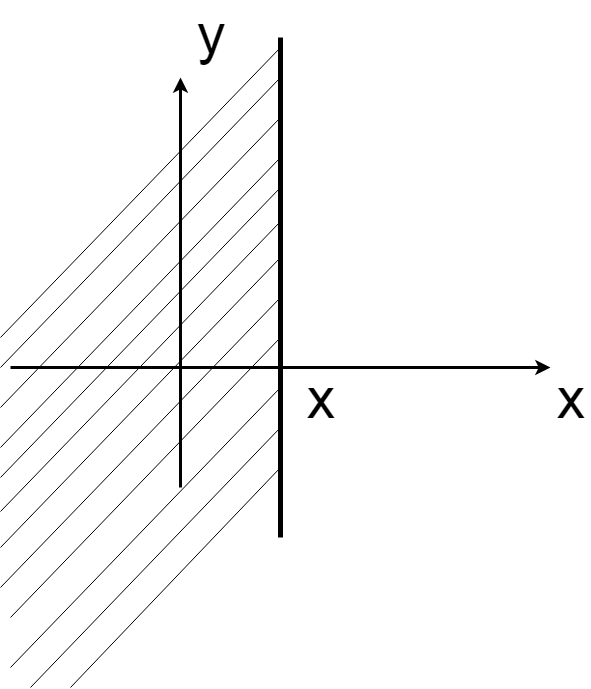
\includegraphics[scale=0.3]{pg30.png}\\	
\begin{figure}[!h]

\begin{tikzpicture}
   \begin{axis}[ ticks=none,xmin=-3, xmax=4, ymin=-3, ymax=3,
     axis y line=middle,
     axis x line=middle,
     y label style={at={(axis description cs:.45,1)},anchor=south, font = \normalsize},
     axis line style={->},
     x label style = {font = \normalsize},
     xlabel=$\large x$, ylabel=$\large y$,
     scale=0.5]
\draw[thick] (400,600) --(400,0);
\draw (400,550) --(200,450);
\draw (400,500) --(200,400);
\draw (400,450) --(200,350);
\draw (400,400) --(200,300);
\draw (400,350) --(200,250);
\draw (400,300) --(200,200);
\draw (400,250) --(200,150);
\draw (400,200) --(200,100);
\draw (400,150) --(200,50);
\draw (400,100) --(200,0);
\draw[fill=black!10!black] (400,300) circle (0.2ex);
\node [right] at (400,330) {$x$};
\end{axis}
\end{tikzpicture}
\caption{График $F_1(x)$}
\end{figure}\\
\noindent
$F_2(y):$\\
%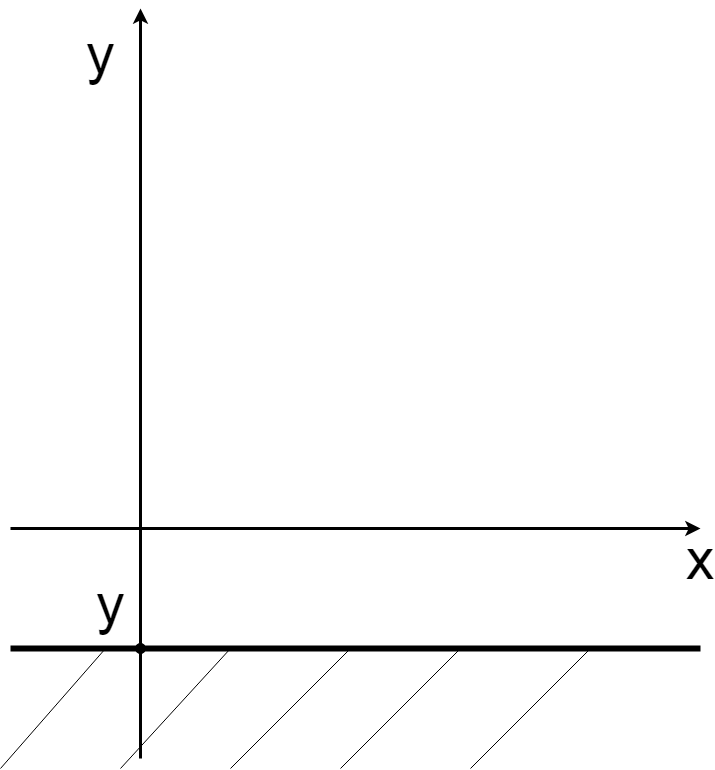
\includegraphics[scale=0.3]{pg30num3.png}\\	
\begin{figure}[!h]
\begin{tikzpicture}
   \begin{axis}[  ticks=none,
	xmin=-3, xmax=4, ymin=-3, ymax=3,
     axis y line=middle,
     axis x line=middle,
     y label style={at={(axis description cs:.45,1)},anchor=south,  font = \normalsize},
     x label style={font = \normalsize},
     axis line style={->},
     xlabel=$\large x$, ylabel=$\large y$,
     scale=0.5]
\draw[thick] (650,400) --(0,400);
\draw (600,400) --(500,100);
\draw (550,400) --(450,100);
\draw (500,400) --(400,100);
\draw (450,400) --(350,100);
\draw (400,400) --(300,100);
\draw (350,400) --(250,100);
\draw (300,400) --(200,100);
\draw (250,400) --(150,100);
\draw (200,400) --(100,100);
\draw (150,400) --(50,100);
\draw (100,400) --(0,100);
\draw[fill=black!10!black] (300,400) circle (0.2ex);
\node [right] at (300,435) {$y$};
\end{axis}
\end{tikzpicture}
\caption{График $F_2(y)$}
\end{figure}\\
2)$F(x, y)$ неубывающая функция по каждому аргументу.\\
3)$F(x, -\infty) = F(-\infty, y) = F(-\infty, -\infty) = 0$\\
4)$F(\infty, \infty) = 1$\\
\textbf{Пример}\\
По мишени производится один выстрел, вероятность попадания = $\frac{3}{4}$, $X$ --  число попаданий , $Y$ -- число промахов, $F(x, y)=$ ?.\\
\begin{tabular}[b]{ | l | l |  l |  }
\hline
\backslashbox{$y$}{$x$}&$0$&1\\
\hline
$0$&$0$&$\frac{3}{4}$\\
\hline
$1$&$\frac{1}{4}$&$0$\\
\hline
\end{tabular}\\
\\
\\
\begin{figure}[!h]
\begin{picture}(100,100)
\put(70, 10){\vector(0, 3){80}}
\put(50, 30){\vector(4, 0){130}}

\put(60, 85){\makebox(10, 0){$Y$}}
\put(170, 20){\makebox(10, 0){$X$}}
\put(70, 60){\line(1, 0){70}}	
\put(90, 30){\line(0, 1){70}}	
\put(0, 40){\makebox(10, 0){$F(x, y)=$}}
\put(55, 20){\makebox(10, 0){$0$}}
\put(120, 20){\makebox(10, 0){$0$}}
\put(55, 40){\makebox(10, 0){$0$}}
\put(75, 40){\makebox(10, 0){$0$}}
\put(75, 70){\makebox(10, 0){$\frac{1}{4}$}}
\put(100, 40){\makebox(10, 0){$\frac{3}{4}$}}
\put(100, 70){\makebox(10, 0){$1$}}
\put(85, 20){\makebox(10, 0){$1$}}
\put(60, 60){\makebox(10, 0){$1$}}
\put(90, 30){\circle*{3}}
\put(70, 60){\circle*{3}}
\end{picture}
\caption{График $F(x, y)$}
\end{figure}\\
Дискретная система случайных величин $X,Y$ характеризуется таблицей распределения : $p_{ij} = P(X=x_i, Y = y_i)$\\
\begin{tabular}[b]{ | l | l |}
\hline
\backslashbox{$Y$}{$X$}&$x_i$\\
\hline
$y_i$&$p_{ij}$\\
\hline
\end{tabular}
%страница 31
\begin{center}
$\textbf{Совместная плотность вероятности системы случайных величин}$
\end{center}
\begin{figure}[!h]
\begin{tikzpicture}
   \begin{axis}[ ticks=none,xmin=-5, xmax=9, ymin=-3, ymax=7,
     axis y line=middle,
     axis x line=middle,
     width=0.8\textwidth,
     y label style={at={(axis description cs:.45,1)},anchor=south, font = \normalsize},
     axis line style={->},
     x label style = {font = \normalsize},
     xlabel=$\large x$, ylabel=$\large y$,
     scale=0.5]
\tikzstyle{every node}=[font=\small]
\draw[thick] (640,500) --(640,0);
\draw[thick] (740,540) --(0,540);
\draw[thick](740,540) --(740,0);
\draw[thick] (740,440) --(0,440);
\draw[thick] (640,540) --(640,0);
\draw[thick] (640,440) --(740,540);
\draw[thick] (640,470) --(710,540);
\draw[thick] (640,500) --(680,540);
\draw[thick] (670,440) --(740,510);
\draw[thick] (700,440) --(740,480);

\draw[fill=black!10!black] (500,440) circle (0.2ex);
\draw[fill=black!10!black] (500 ,540) circle (0.2ex);
\draw[fill=black!10!black] (640,300) circle (0.2ex);
\draw[fill=black!10!black] (740,300) circle (0.2ex);
\node [below left] at (520,430) {$ y $};
\node [below left] at (510,693) {$ y + \Delta y$};
\node [below left] at (630,290) {$x$};
\node [below right] at (720,310) {$x + \Delta x$};
\end{axis}
\end{tikzpicture}
\caption{График совместных величин}
\end{figure}
Для непрерывной случайной величины : $f(x, y) =  \displaystyle{  \lim_{\substack{{\Delta y\to{\infty}}\\
												        {\Delta x\to{\infty}}}}}$
$\frac{P((X;Y)\in D)}{\Delta x \Delta y}$ -- совместная плотность вероятности (вероятностное распределение).\\
Пусть $F(x, y)$ дважды непрерывно дифференцируема. \\
$P((X, Y) \in D) = F(x + \Delta x, y + \Delta y) -  F(x + \Delta x, y ) -  F(x , y + \Delta y) +  F(x , y )$ \\
$f(x, y)=  \displaystyle{  \lim_{\substack{{\Delta y\to{\infty}}\\ {\Delta x\to{\infty}}}}} \frac{ F(x + \Delta x, y + \Delta y) -  F(x + \Delta x, y ) -  F(x , y + \Delta y) +  F(x , y )}{\Delta x \Delta y} = \\ = \frac{\delta^2 F(x, y)}{\delta x \delta y}$\\
Из  определения следует, что $P((X, Y) \in \Omega)$  = $\displaystyle{\iint\limits_{\Omega}} f(x, y)dxdy$\\
$F(x, y) = \displaystyle{\int\limits_{-\infty}^{x} \int\limits_{-\infty}^{y} f(x, y) dx dy}$\\
Свойства:\\
1)$f(x, y) \geq 0$\\
2)$\iint\limits_{-\infty}^{\infty} f(x, y) dxdy = 1$\\
\textbf{Пример} \\
$f(x, y) = \frac{1}{\pi^2(1+x^2)(1+y^2)}$\\
$F(x, y) = \frac{1}{\pi^2} \displaystyle{\int\limits_{-\infty}^{x}  \int\limits_{-\infty}^{y}} \frac{dxdy}{(1+x^2)(1+y^2)} = (\frac{1}{\pi}\arctg x + \frac{1}{2}) (\frac{1}{\pi}\arctg y + \frac{1}{2})$\\
$P(0\leq x \leq 1; -1 \leq y \leq 1) = \frac{1}{\pi^2} \displaystyle{\int\limits_{0}^{1}dx\int\limits_{-1}^{1} dy \frac{dxdy}{(1+x^2)(1+y^2)}} = \frac{1}{8}$
\begin{center}
$\textbf{Плотность вероятности компонент}$\\
(маргинальные (частные) плотности)
\end{center}
$F_1(x) = F(x, \infty)  = \displaystyle{\int\limits_{-\infty}^{x}\int\limits_{-\infty}^{\infty}f(x, y)dxdy}$\\
$f_1(x) = F_1'(x) = \displaystyle{\int \limits_{-\infty}^{\infty}} f(x, y) dy$\\
Аналогично: $f_2(y) = F_2'(y) = \displaystyle{\int \limits_{-\infty}^{\infty}} f(x, y) dx$\\
Определим условные плотности вероятности: $f_2(y|x) = \frac{f(x,y)}{f_1(x)};f_1(x|y) = \frac{f(x,y)}{f_2(y)}$\\
Соотношение $f(x, y) = f_1(x) f_2(y|x)$ соответствует теореме умножения вероятностей. Смысл: $f_2(y|x)$ -- это плотность распределения случайной величины $Y$ при условии, что $X=x$.\\
Для дискретной случайной величины: $p_i = \sum\limits_{j} p_{ij}$\\
$P(X=x_i) =  \sum\limits_{j} P(X=x_i, Y=y_j)$\\
%страница 32
\textit{\textbf{Определение}}\\
Случайные величины $X, Y$ называются независимыми, если $f(x, y) = f_1(x)f_2(y)$ (для непрерыных случайных величин)\\
$ P(X = x_i, Y = y_j) = P(X=x_i) P(Y=y_j)$ (для дискретных случайных  величин)\\
Это означает, что $f_2(y|x) = f_2(y)$ и $f_1(x|y) = f_1(x)$, то есть закон распределения случайной величины $Y$ не зависит от того, какое значение приняла величина $X$.\\
\textbf{Пример} \\
$f(x, y) = \frac{1}{\pi^2(1+x^2)(1+y^2)}$, $f_1(x) = \frac{1}{\pi(1+x^2)}$, $f_2(y) = \frac{1}{\pi(1+y^2)}$ -- независимые случайные величины.
\begin{center}
$\textbf{Функции распределения и плотности систем из n случайных величин}$\\
\end{center}
 $F(x_1, x_2, .\ .\ . x_n) = P(X_1 < x_1, X_2 < x_2,\ .\ .\ .,X_n < x_n)$\\
Свойства те же, что и при $n = 2$.\\
$f(x_1, x_2, \ .\ .\ .x_n) = \frac{\delta^nF(x_1, x_2, .\ .\ . x_n)}{\delta x_1 \delta x_2 .\ .\ . \delta x_n}$ \\
$F_1(x_1) = F(x_1, \infty, \ .\ .\ ., \infty)$\\
$f_1(x_1) =  \displaystyle{\int \limits_{-\infty}^{\infty}}.\ .\ .\  \displaystyle{\int \limits_{-\infty}^{\infty}} f(x_1, .\  .\ , x_n) dx_2\ .\ .\ dx_n$\\
Случайные величины независимы, если $f(x_1, x_2, .\ .\ .\ x_n)  = f_1(x_1)  f_2(x_2)\ .\ .\ . f_n(x_n)$\\
%страница 33
\subsection{Числовые характеристики системы из двух случайных величин}
Основные характеристики системы $(X, Y)$:\\
$M(X), M(Y), D(X), D(Y), K_{XY}$ -- они уже определены, но их можно находить, не вычисляя $f_1(x), f_2(y)$.\\
\begin{tabular}[b]{ | l | l |  }
\hline
 Дискретная & Непрерывная   \\
  случайная величина   & случайная  величина   \\
\hline
$M(X) = \displaystyle{ \sum \limits_{i, j}^{}} x_i p_{i, j} $ & $\displaystyle{\iint\limits_{-\infty}^{\infty}} xf(x, y)dxdy$ \\
\hline
$M(Y) = \displaystyle{ \sum \limits_{i, j}^{}} y_j p_{i, j} $ & $\displaystyle{\iint\limits_{-\infty}^{\infty}} yf(x, y)dxdy$ \\
\hline
$D(X) = \displaystyle{ \sum \limits_{i, j}^{}} (x_i - M(X))^2 p_{i,j} $ & $\displaystyle{\iint\limits_{-\infty}^{\infty}} (x - M(X))^2 f(x, y) dxdy$ \\
&=  $\displaystyle{\iint\limits_{-\infty}^{\infty}} x^2 f(x, y) dxdy$\\
\hline
$K_{X, Y} = \displaystyle{ \sum \limits_{i, j}^{}} (x_i - M(X))(y_j - M(Y)) p_{ij}$ & $\displaystyle{\iint\limits_{-\infty}^{\infty}} (x - M(X))(y - M(Y)) f(x, y) dxdy$\\
$=cov(X, Y)$ & \\
\hline
\end{tabular}\\
$\textbf{Теорема}$\\
Корреляционный момент независимых случайных величин равен нулю\\
\underline{Доказательство:}\\
Для  непрерывных случайных величин:\\
Они независимы, значит, $f(x, y) = f_1(x)f_2(y)$\\
$K_{XY} = \displaystyle{\int\limits_{-\infty}^{\infty}} (x-M(X))f_1(x)dx \displaystyle{\int\limits_{-\infty}^{\infty}} (y-M(Y)) f_2(y)dy = 0$\\
$r_{XY} = \frac{K_{XY}}{\sigma_x \sigma_y}$, $\sigma_x = \sqrt{D(X)}$, $\sigma_y = \sqrt{D(Y)}$.\\
\begin{flushright}\(\blacksquare\)\end{flushright}
\textbf{Пример}
%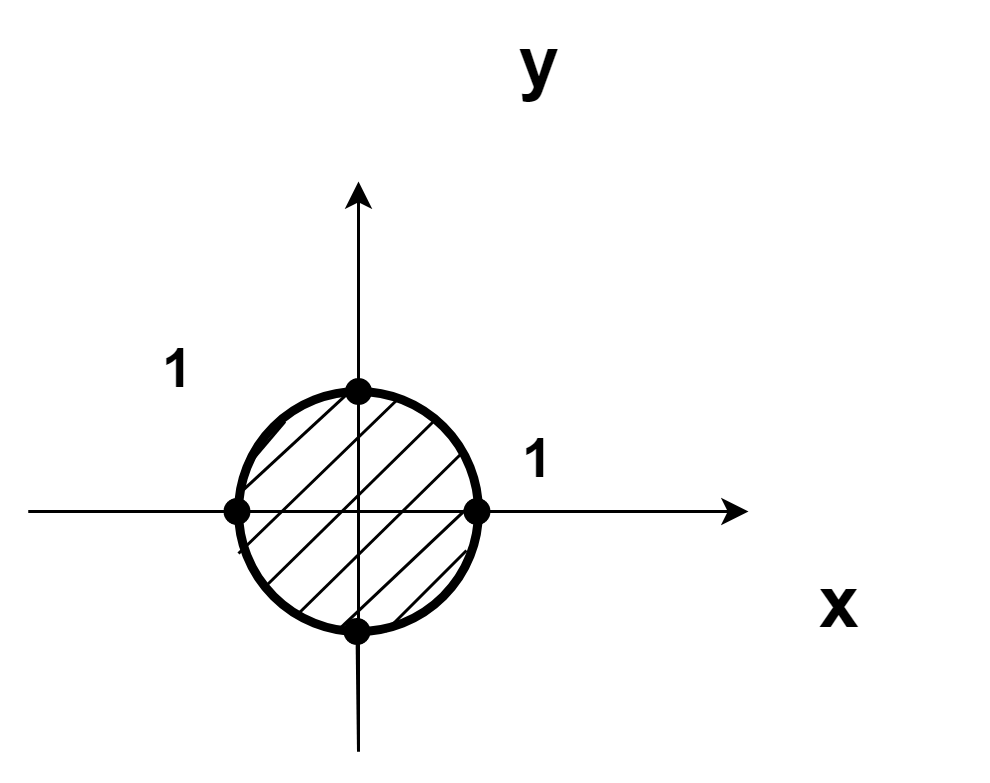
\includegraphics[scale=0.2]{UntitledDiagram3.png}\\
\begin{figure}[!h]
\begin{tikzpicture}[scale=0.6]
   \begin{axis}[ xmin=-2, xmax=2, ymin=-2, ymax=2,
     ticks=none,
     axis y line=middle,
     axis x line=middle,
label style={font=\Large},
     y label style={at={(axis description cs:.55,0.9)},anchor=south },
     x label style={at={(axis description cs: 0.96,0.5)},anchor=south },
%y label style={ticks=none,at={(axis description cs:0.2,10)},rotate=270,anchor=south},
     axis line style={->},
     xlabel=$x$, ylabel=$y$,
   ]
\node [black, right, scale = 1.2] at (axis cs: 0.04, 1.2) {$1$ }; %,scale = 0.8
 \node [black,above right, scale  = 1.2] at (axis cs: 0.88, 0) {$1$ };
\end{axis} 
\draw[fill=black!10!black] (3.45,4.35) circle (0.3ex);
 \draw [black, thick] (3.45,2.85) circle [radius=1.5];
\pattern[pattern=north east lines, pattern color=black]  (3.45,2.85) circle [radius = 1.5];
 \draw [fill=black!10!black] (4.95,2.85)  circle (0.3ex);
\end{tikzpicture}
\caption{График $f(x, y)$}
\end{figure}\\
\begin{equation*} 
f(x, y)=
 \begin{cases}
   \frac{1}{\pi},\    x^2 + y^2 < 1\\
   0 ,\  x^2 + y^2 > 1\\
 \end{cases}
\end{equation*}\\
Величины являются зависимыми (если $X  = 0$, то $Y$ может с равными вероятностями принимать значения на $[-1, 1]$, если $x=1$, то $Y$ может принять одно единственное значение $Y=0$).\\
$M(X)=M(Y) = 0$ по соображениям симметрии.\\
$K_{XY}$ = $\displaystyle{\iint\limits_{C}^{}} xf(x, y)dxdy$ =  $\frac{1}{\pi} \displaystyle{\iint\limits_{C}^{}} xy dxdy$ = $\frac{1}{\pi} \displaystyle{\iint\limits_{C_1}^{}} xy dxdy$+ $\frac{1}{\pi} \displaystyle{\iint\limits_{C_2}^{}} xy dxdy$ +\\+ $\frac{1}{\pi} \displaystyle{\iint\limits_{C_2}^{}} xy dxdy$ + $\frac{1}{\pi} \displaystyle{\iint\limits_{C_3}^{}} xy dxdy$ + $\frac{1}{\pi} \displaystyle{\iint\limits_{C_4}^{}} xy dxdy$ = $0$.\\
(Так как интегралы одинаковы по величине и отличаются знаком.)\\	
То есть независимые следовательно некоррелирующие, обратное неверно.\\
$-1\leq r_{xy} \leq 1$\\
Если $Y=aX+b$, то $r_{XY} = \pm \ 1$\\
Если $a>0$   , то +1, если $a<0$ то $-1$\\
Докажем это позже.\\
\textbf{Пример}\\
а)Вес и рост человека связаны положительной корреляцией\\
б)Возраст взрослого человека и количество волос у него на голове связаны отрицательной корреляцией\\
$\alpha_{k,s} (X,Y) = \sum\limits_{i, j} x_i^k y_j^s p_{ij} =  \displaystyle{\iint\limits_{-\infty}^{\infty}} x^k y^s f(x, y) dx dy  $ -- начальный момент корреляции.\\ 
$\mu_{k,s}(X, T)  \sum\limits_{i, j} (x_i - M(X))^k (y_j - M(Y))^s p_{i j} = \displaystyle{\iint\limits_{-\infty}^{\infty}}(x-M(X))^k(y-M(y))^s f(x, y) dxdy$
%страница 34
\begin{center}
$\textbf{Числовые характеристики систем n случайных величин}$
\end{center}
$X_1, X_2, .\ .\ .\ .\ X_n$ -- их характеристики: $n$ математических ожиданий $(m_1, m_2, \ .\ . \  m_n)$, $n$ дисперсий $(D_1, \ .\ .\ . D_n)$,  $n(n-1)$ корреляционных моментов:\\
$K_{ij} = M((X_i - m_i)(X_j - m_j))$($D_i$ = $K_{ii}$)\\
Корреляционные матрицы K
$$
K=\left(\begin{tabular}{c c c c c}
\(D_1\) & \(K_{12}\) & \(K_{13}\) & \(\ldots\) & \(K_{1n}\) \\
\(K_{21}\) &\( D_2\) & \(K_{13}\) & \(\ldots\) &\( K_{2n}\)\\
\(\vdots\) & \(\vdots\) & \(\vdots\) & \(\ddots\) & \(\vdots\) \\
\(K_{n1}\)& \(K_{n2}\) &\( K_{n3}\) & \(\ldots\) & \(D_n\)\\	
\end{tabular}\right)$$\\
$K_{i, j} = K_{j, i}$, поэтому часто пишут только половину матрицы:\\

$$
K=\left(\begin{tabular}{c c c c c}
\(D_1\) & \(K_{12}\) & \(K_{13}\) & \(\ldots\) & \(K_{1n}\) \\
 &\( D_2\) & \(K_{13}\) & \(\ldots\) &\( K_{2n}\)\\
 &  &  & \(\ddots\) & \(\vdots\) \\
 &  & & & \(D_n\)\\	
\end{tabular}\right)$$\\

Если $X_1, X_2, \ .\ .\ . X_n$-- не коррелированны , то корреляционная матрица:\\
$$
K=\left(\begin{tabular}{c c c c c}
\(D_1\) & \(0\) & \(0\) & \(\ldots\) & \(0\) \\
\(0\) &\( D_2\) & \(0\) & \(\ldots\) &\( 0\)\\
\(\vdots\) & \(\vdots\) & \(\vdots\) & \(\ddots\) & \(\vdots\) \\
\(0\)& \(0\) &\(0\) & \(\ldots\) & \(D_n\)\\	
\end{tabular}\right)$$\\
Коэффициент корреляции $r_{ij} = \frac{k_{ij}}{\sigma_i \sigma_j}$\\
Нормированная корреляционная матрица
$$
K=\left(\begin{tabular}{c c c c c}
\(1\) & \(r_{12}\) & \(r_{13}\) & \(\ldots\) & \(r_{1n}\) \\
\(r_{21}\) &\(1\) & \(r_{23}\) & \(\ldots\) &\( r_{2n}\)\\
\(\vdots\) & \(\vdots\) & \(\vdots\) & \(\ddots\) & \(\vdots\) \\
\(r_{n1}\)& \(r_{n2}\) &\( r_{n3}\) & \(\ldots\) & \(1\)\\
\end{tabular}\right)$$
-- характеризует именно коррелированность, безотносительно  к их рассеиванию.



%страница 35
\subsection{Нормальный закон распределения систем случайных величин}
\noindent
$(X, Y)$ -- нормированные случайные величины.\\
$\displaystyle{ f(x, y) = \frac{1}{2\pi\sigma_x\sigma_y\sqrt{1-r^2}} e^{{-\frac{1}{2(1-r^2)}\cdot \left(\frac{(x-m_x)^2}{\sigma_x^2} + \frac{2r(x-m_x)(y-m_y)}{\sigma_x\sigma_y} + \frac{(y-m_y)^2}{\sigma_y^2}\right)}}}$\\
Можно показать, что $m_x, m_y$ -- математические ожидания,\\ $\sigma_x ,\sigma_y$ -- среднеквадратичные  отклонения, $r$  -- коэффициент корреляции $X$ и $Y$.\\
$\textbf{Теорема}$\\
Для нормального распределения случайной величины $X$ и $Y$ независимость эквивалентна некоррелированности.\\
\underline{Доказательство:}\\
Из независимости следует некоррелируемость для любой случайной величины.\\
Пусть $X$, $Y$ -- нормированны, и $r=0$, следовательно:\\ $f(x, y) =\frac{1}{2\pi\sigma_x\sigma_y}e^{-\frac{(x-m_x)^2}{2\sigma_x^2}}e^{-\frac{(y-m_y)^2}{2\sigma_y^2}}=f_1(x)f_2(x)$,  то есть $X$ и $Y$ -- независимы.\\
\begin{flushright}\(\blacksquare\)\end{flushright}
\begin{center}
$\textbf{Регрессия}$
\end{center}
Рассмотрим условную плотность вероятности $f_2(y|x)$. Введем условное математическое ожидание:
$M(Y|X=x) = \displaystyle{\int \limits_{-\infty}^{\infty} y f_2(y|x) dy = \frac{1}{f_1(x)} \int \limits_{-\infty}^{\infty} y f(x,y) dy }$,\\в предположении, что интеграл сходится абсолютно.\\
$M(Y|X)$ -- это случайная величина (она является функцией только от $X$, а не от $Y$, которая называется регрессией $Y$ на $X$).\\
Это соотношение не определено, когда $f_1(x) = 0$. Пусть в этом случае \\
$M(Y|X=x) = 0$, тогда $M(Y|X=x)$ определено, когда $f_1(x)\ =\ 0$. Пусть в этом случае $M(Y|X=x) = 0$, тогда $M(Y|X)$ определено для любой непрерывной плотности распределения.  Можно ввести аналогичным образом условную дисперсию.\\$Var(Y|X) = D(Y|X)$.\\
\\
Для нормального закона распределения:\\
 $f_2(y|x) = \frac{1}{\sigma_y \sqrt{1 - r^2} \sqrt{2\pi}} \displaystyle{  e^{{-\frac{1}{2(1-r^2)}\cdot \left(\frac{(x-m_x)^2}{\sigma_x^2}  -r \frac{(y-m_y)^2}{\sigma_y^2}\right)}}  	}= \displaystyle{  \frac{  e^{{-\frac{1}{2(1-r^2)}\cdot \left (\frac{(x-m_x)^2}{\sigma_x^2}  -r \frac{(y-m_y)^2}{\sigma_y^2}\right )}} }{\sigma_y \sqrt{1 - r^2} \sqrt{2\pi}}}$\\
То есть это плотность нормального закона с $m_{y|x} = m_y + r \frac{\sigma_y}{\sigma_x} (x - m_x)$  и среднеквадратичное отклонения $\sigma_{y|x} = \sigma_{y} \sqrt{1-r^2}$ \\
То есть от $x$ в условном законе зависит лишь $m_{y|x}$, но не $\sigma_{y|x}$. Откладывая  $m_{y|x}$ на оси ординат при различных $x$ получим линию регрессии $Y$  на $X$: $y=m_y + r\frac{\sigma_y}{\sigma_x}(x-m_x)$. Для нормального распределения регрессия линейна.\\
\textbf{Пример}\\
%страница 36
Гальтона -- характеризует эмпирическое значение формул линейной регрессии. Пусть $X_1$ и $X_2$ -- характеризуют рост (измеренный по отклонению от среднего в сантиметрах) соответственно отцов и сыновей в некоторой популяции. Рост случайно выбранного сына -- нормальная случайная величина с $M(X_2) = 0$ и $D(X_2) = \sigma_2^2$,
отца -- с $M(X_1) = 0, D(X_1) = \sigma_1^2$. Но в подпопуляции сыновей, отцы которых имеют фиксированный рост $x$, рост сыновей представляется нормальной величиной с (по формулам регрессии) математическим ожиданием  $r\frac{\sigma_2}{\sigma_1} x$ и дисперсией $\sigma_2^2(1-r^2) < \sigma_2^2$.\\
Таким образом, регрессия $X_2$ на $X_1$ показывает как много статистической информации относительно $X_2$ содержится в наблюдении над $X_1$.\\
%страница 37
\newpage
\section{Функции случайных величин}
\subsection{Числовые характеристики функций случайных величин}
\noindent

$Y = \varphi(X)$, $M(Y) = M(\varphi(X))$\\

\begin{tabular}[b]{ | l | l |  l | l | }
\hline
$x_i$&$x_1$&$x_2$&...\\
\hline
$p_i$&$p_1$&$p_2$&...\\
\hline
\end{tabular}\\

\begin{tabular}[b]{ | l | l |  l | l | }
\hline
$\varphi(x_i)$&$\varphi(x_1)$&$\varphi(x_2)$&...\\
\hline
$p_i$&$p_1$&$p_2$&...\\
\hline
\end{tabular}\\
Для непрерывной  случайной величины: $M(\varphi(X, Y)) = \displaystyle{\int \limits _{-\infty}^{\infty} } \varphi(x) f(x) dx$\\
Для дискретной случайной  величины: $M(\varphi(X, Y)) = \displaystyle{\sum \limits _{i,j}^{} } \varphi(x_i, y_j) p_{i, j}  dx$\\
\textbf{Пример} \\
На плоскости задан отрезок длинны $l$, вращающаяся случайным образом так, что все направления одинаково вероятны. Найти среднее значение длинны проекции отрезка на неподвижную ось.\\
$Y = l \abs{\cos \alpha}$, $\alpha$ распределенна равномерно от 0 до $2\pi$\\
\\
$M(l\abs{\cos \alpha}) = \displaystyle{\int \limits_{0}^{2\pi}} l\abs{\cos \alpha} \frac{d\alpha}{2\pi}=\frac{2l}{\pi} \displaystyle{\int \limits_{0}^{2\pi}} \cos \alpha  d\alpha = \frac{2l}{\pi}$\\
$D(l\abs{\cos \alpha}) = \frac{4}{2\pi}  \displaystyle{\int \limits_{0}^{\frac{\pi}{2}}} l^2\cos^2 \alpha d\alpha  - \frac {4l^2}{\pi^2}= \frac{2l^2}{\pi} \displaystyle{\int \limits_{0}^{\frac{\pi}{2}}} (\frac{1}{2} + \frac{1}{2} \cos 2\alpha) d\alpha - \frac{4l^2}{\pi^2} = \frac{l^2}{2} - \frac{4l^2}{\pi^2}$\\
\textbf{Пример}\\ В процессе слежения радиолокатором за определенным объектом пятно изображающее объект, все время удерживается в пределах экрана (круг радиуса $R$)  и занимает на нем случайное положение с постоянной плотностью вероятности. Найти среднее расстояние до центра экрана.\\
$f(x, y) = \frac{1}{\pi R^2}$\\
$M(r) = \displaystyle{\iint\limits_{K}} \sqrt{x^2+y^2}\frac{dxdy}{\pi R^2} = \frac{1}{\pi R^2} \displaystyle{\int\limits_{0}^{2\pi}} d \varphi \displaystyle{\int\limits_{0}^{R}} \rho^2 d \rho = \frac{l}{3} R$
%страница 38
\begin{center}
$\textbf{Теоремы о числовых характеристиках}$
\end{center}
1)$M(C) = C$\\
2)$D(C) = 0$\\
3)$M(cX) = cM(X)$\\
\underline{Доказательство:}\\
$M(cX) = \displaystyle{\int\limits_{-\infty} ^{\infty}} c x f(x) dx = c \displaystyle{\int \limits_{-\infty} ^{\infty}} x f(x) dx = xM(X)$
\begin{flushright}\(\blacksquare\)\end{flushright}
4)$D(cX) = c^2 D(X)$\\
\underline{Доказательство:}\\
$D(cX)=M((cX - M(cX))) = M((cX - c M(X))^2) = M(c^2(X-M(X))^2) =\\= c^2M((X-M(X))^2) = c^2 D(X)$
\begin{flushright}\(\blacksquare\)\end{flushright}
5)$M(X+Y) = M(X) + M(Y)$,  $M(\sum x_i) = \sum M(x_i)$\\
\underline{Доказательство:}\\
$M(X + Y) =  \displaystyle{\iint \limits_{-\infty} ^{\infty}} (x+y)f(x,y) dxdy$ = $\displaystyle{\iint \limits_{-\infty} ^{\infty}} xf(x,y) dxdy + \displaystyle{\iint \limits_{-\infty} ^{\infty}} yf(x,y) dxdy$ =\\= $\displaystyle{\int\limits_{-\infty}^{\infty} } dx x \displaystyle{\int\limits_{-\infty}^{\infty} } f(x, y) dy $ +  $\displaystyle{\int\limits_{-\infty}^{\infty} } dy y \displaystyle{\int\limits_{-\infty}^{\infty} } f(x, y) dx $ = $\displaystyle{\int\limits_{-\infty}^{\infty} } dx x f_1(x) + \displaystyle{\int\limits_{-\infty}^{\infty} } dyy f_1(y)$ =\\= $M(X) + M(Y)$
\begin{flushright}\(\blacksquare\)\end{flushright}
6)$M(\sum \limits a_i X_i + b) = \sum \limits a_i M(x_i) + b$\\
7)$D(X + Y) = D(X) + D(Y) + 2 K_{XY}$\\
\underline{Доказательство:}\\
$Z=X+Y$. Перейдем к центрированным величинам.
%доделать с кружочками.
\begin{flushright}\(\blacksquare\)\end{flushright}
8)$\displaystyle{D\left (\sum_{i = 1}^{n}a_iX_i + b\right )} =  \displaystyle{\sum_{i = 1}^{n}}  a_i^2 D(X_i) + 2 \displaystyle{\sum_{i <j}^{n}}a_ia_jK_{i,j}$\\
\underline{Доказательство:}\\
$Y_i = a_i X_i$,\\
 $ \displaystyle{\sum_{i = 1}^{n}}a_iX_i + b =  \displaystyle{\sum_{i = 1}^{n}}Y_i + b$, следовательно  $\displaystyle{D\left (\sum_{i = 1}^{n}a_iX_i + b\right )}  = \displaystyle{\sum_{i = 1}^{n}} D(Y_i) + \displaystyle{\sum_{i < j}^{}} K_{i,j} ^y =\\= \displaystyle{\sum_{i = 1}^{n}}a_i^2D(X_i) + 2 \displaystyle{\sum_{i  < j}} K_{i,j}^{y}$
\begin{flushright}\(\blacksquare\)\end{flushright}
9)$M(XY)=M(X)M(Y)+K_{XY}$\\
\underline{Доказательство:}\\
$K_{XY} = M(XY) = M((X-m_x)(Y-m_y)) = M(XY)  - m_xM(Y) - m_y M(X) +\\+ m_xm_y  = M(XY) - M(X)M(Y)$
\begin{flushright}\(\blacksquare\)\end{flushright}
%страница 39
Для двух некоррелирующих величин: $M(XY) = M(X)M(Y)$. Если произведение более 2х случаных величин, то некоррелируемости недостаточно (требуется зануление некоторых высших смешанных моментов), что заведомо выполняется при независимости случайных величин.\\
Независимы, следовательно $\displaystyle{ M(\prod_{i}x_i) = \prod_{i} M(x_i)}$\\
10)Для независимых случайных величин $X,\ Y,\ Z$.\\
$D(XY)=D(X)D(Y) + m_xD(Y) + m_y^2D(X)$ \\
\underline{Доказательство:}\\
$XY=Z$, $D(XY)=M(Z^2)=((Z-m_Z)^2) = M((XY-m_xm_y)^2)$
Величины независимы, следовательно $m_z=m_xm_y$\\
$M((XY-m_xm_y)^2 = M(X^2Y^2) - 2m_xm_y M(XY) + m_x^2 m_y^2$\\
$X, Y$ независимы, следовательно $X^2$ и $Y^2$ независимы, следовательно $M(X^2Y^2) =M(X^2)M(Y^2)$ и $M(XY) = m_x m_y$, следовательно \\
$D(XY) = M(X^2)M(Y^2) - m_x^2 m_y^2$, $M(X^2) = D(X) + m_x^2$; $M(Y^2) = D(Y) + m_y^2$ , следовательно утверждение теоремы верно.
\begin{flushright}\(\blacksquare\)\end{flushright}
%страница 40
\begin{center}
$\textbf{Применение теоремы о числовых характеристиках.}$
\end{center}
$Y=aX+b$, следовательно, $r_{XY}=\pm 1$\\
\underline{Доказательство:}\\	
$K_{XY}$ = $M(XY) = M((X-m_k)(Y-m_y))  = M((X-m_x)(aX + b - am_x - b)) =\\ = aM((X-m_x)^2) = aD_x$\\
$D_y = D(aX+b)  = a^2 D_x$, $\sigma_x$ = $\abs{a} \sigma_x$
\begin{equation*} 
r_{XY} = \frac{aD_x}{\sigma_x \sigma_y} = \frac{aD_x}{\sigma_x \abs{a} \sigma_x} = \frac{a}{\abs{a}}=
 \begin{cases}
  +1, a > 0\\
   -1, a < 0\\
 \end{cases}
\end{equation*}
\begin{flushright}\(\blacksquare\)\end{flushright}
$\abs{r_{XY}} \leq 1$\\
\underline{Доказательство:}\\	
Пусть $Z = \sigma_y X \pm \sigma_xY$\\
$D(Z) = \sigma_y^2 D_x + \sigma_x^2D_y \pm 2\sigma_2 \sigma_y K_{xy} = 2 \sigma_x^2 \sigma_y^2 \pm  2 \sigma_x \sigma_y K_{xy} \geq 0$\\
 $2\sigma_x^2 \sigma_y^2 \pm  2 \sigma_x \sigma_y K_{xy} \geq 0$\\
 $\sigma_x^2 \sigma_y^2 \pm  K_{xy} \geq 0$, следовательно $\abs{K_{xy}} \leq \sigma_x \sigma_y$, следовательно $\abs{r_{xy}} \leq 1$\\
\begin{flushright}\(\blacksquare\)\end{flushright}
%страница 41
\subsection{Законы распределения функций случайной величины}
\noindent
$Y=\varphi(x)$. Пусть $\varphi$ непрерывна и дифференцируема. $X$ -- непрерывная случайная величина. Пусть значения случайной величины $X$ лежат на $(a, b)$, и $\varphi$ на $(a, b)$ монотонна.\\
a) $\varphi$ монотонно возрастает на $(a, b)$. $f(x)$ -- плотность вероятности $X$, $g(y)$ -- плотность вероятности $Y$, $G(y)$ -- функция распределения $Y$. \\$G(y) = P(Y < y) = P(a < X < x) $(так как $\varphi$ -- возрастающая функция.)\\
$P(a<X<x) = \displaystyle{\int \limits_{a}^{x}} f(x) dx$.\\
\\
\\
\begin{figure}[H]
\begin{tikzpicture}
   \begin{axis}[ xmin=0, xmax=4, ymin=0.5, ymax=3,
     ticks=none,
     axis y line=middle,
     axis x line=middle,
clip mode=individual ,
label style={font=\large},
%     y label style={at={(axis description cs:0.1,12)},anchor=south },
    x label style={at={(axis description cs: 0.98,0.02)},anchor=south },
y label style={at={(axis description cs: 0.05,0.93)},anchor=south },
%y label style={ticks=none,at={(axis description cs:0.2,10)},rotate=270,anchor=south},
     axis line style={->},
 width=0.4\textwidth,
     xlabel=$x$, ylabel=$y$,
   ]
     \addplot[black, samples=100, smooth, unbounded coords=discard,domain=1:pi/2+ 1] {sin(deg(x-1)) +1}; 
	\node [black,below, -latex] at (axis cs:1.1,0.5) {$a$};
	\node [black,below, -latex] at (axis cs:pi/2 + 1,0.5) {$b$};	
	\node [black,below, -latex] at (axis cs:pi/4 + 1-0.1,0.5) {$x$};

		\node [black,left, -latex] at (axis cs:0,0.70710 + 1) {$y$};		

	\draw[dashed] (axis cs:1.1, 0.5) -- (axis cs:1.1,  0.0998 + 1);
	\draw[dashed] (axis cs:pi/2 + 1 -0.1, 0.5) -- (axis cs:pi/2 + 1 - 0.1, 1.995);
	\draw[dashed] (axis cs:pi/4 + 1, 0.5) -- (axis cs:pi/4 + 1, 0.70710 + 1);
	\draw[dashed] (axis cs:0, 0.70710 + 1) -- (axis cs:pi/4 + 1, 0.70710 + 1);
	\draw [black, fill] (axis cs:1+0.1,0.5)   circle (0.15ex);
	\draw [black, fill] (axis cs:pi/2 + 1-0.1,0.5)  circle (0.15ex);

	\draw [black, fill] (axis cs:0,0.70710 + 1)  circle (0.15ex);



	\draw [black, fill] (axis cs:pi/4 + 1,0.5)  circle (0.15ex);
	\draw [black, fill] (axis cs:1+0.1, 0.0998 + 1)   circle (0.15ex);
	\draw [black, fill] (axis cs:pi/2 + 1-0.1,1.995)  circle (0.15ex);
	\draw [black, fill] (axis cs:pi/4 + 1,0.70710 + 1)  circle (0.15ex);
\end{axis}
\end{tikzpicture}
\caption{График $y = \varphi(x)$}
\end{figure}
\noindent
Пусть $\psi(y)$ -- обратная функция к $\varphi(x)$.
Тогда $G(Y) =   \displaystyle{\int \limits_{a}^{\psi(y)}} f(x) dx$. $g(y) = G'(y) =\\= f(\psi(y))\psi'(y)$\\
б)$\varphi$ -- монотонно убывает на $(a, b)$\\
$G(y) = P(Y < y) = P(x< X < b) =  \displaystyle{\int \limits_{\psi(y)}^{b}} f(x) dx$\\
$g(y) = G'(y) = -f(\psi(y)$ .
\begin{figure}[H]
\begin{picture}(100,110)
\put(10, 10){\vector(0, 4){100}}
\put(10, 10){\vector(4, 0){120}}
\put(0, 120){\makebox(0, 0) {$y$}}
\put(100, 0){\makebox(0, 0) {$x$}}
\put(100, 40){\makebox(0, 0) {$y=\varphi(x)$}}
\qbezier(20,70)(30,40)(70,30)
\put(30, 10){\line(0, 1) {3}}
\put(30, 16){\line(0, 1) {3}}
\put(30, 22){\line(0, 1) {3}}
\put(30, 28){\line(0, 1) {3}}
\put(30, 34){\line(0, 1) {3}}
\put(30, 40){\line(0, 1) {3}}
\put(30, 46){\line(0, 1) {3}}


\put(30, 10){\circle*{2}}
\put(40, 10){\circle*{2}}
\put(60, 10){\circle*{2}}

\put(10, 43){\circle*{2}}
\put(10, 33){\circle*{2}}
\put(10, 50){\circle*{2}}


\put(12, 50){\line(1, 0) {3}}
\put(18, 50){\line(1, 0) {3}}
\put(24, 50){\line(1, 0) {3}}



\put(30, 0){\makebox(0, 0) {$a$}}
\put(40, 10){\line(0, 1) {3}}
\put(40, 16){\line(0, 1) {3}}
\put(40, 22){\line(0, 1) {3}}
\put(40, 28){\line(0, 1) {3}}
\put(40, 34){\line(0, 1) {3}}
\put(40, 40){\line(0, 1) {3}}

\put(40, 0){\makebox(0, 0) {$x$}}
\put(0, 43){\makebox(0, 0) {$y$}}

\put(10, 43){\line(1, 0) {3}}
\put(16, 43){\line(1, 0) {3}}
\put(22, 43){\line(1, 0) {3}}
\put(28, 43){\line(1, 0) {3}}
\put(34, 43){\line(1, 0) {3}}

\put(13, 33){\line(1, 0) {3}}
\put(19, 33){\line(1, 0) {3}}
\put(25, 33){\line(1, 0) {3}}
\put(31, 33){\line(1, 0) {3}}
\put(37, 33){\line(1, 0) {3}}
\put(43, 33){\line(1, 0) {3}}
\put(49, 33){\line(1, 0) {3}}
\put(55, 33){\line(1, 0) {3}}


\put(60, 10){\line(0, 1) {3}}
\put(60, 16){\line(0, 1) {3}}
\put(60, 22){\line(0, 1) {3}}
\put(60, 28){\line(0, 1) {3}}
\put(60, 0){\makebox(0, 0) {$b$}}
\end{picture}
\caption{График $y = \varphi(x)$}
\end{figure}
\noindent
Общая формула: $g(y) = f(\psi(y)) \abs{\psi(y)}$\\
\textbf{Пример} \\
\begin{figure}[H]
\begin{tikzpicture}
  \draw[] (1, 0) -- (1, 4);
 \draw[dashed] (1, 2) -- (5, 2);
 \draw[dashed] (1, 4) -- (5, 2);
 \node [black, right] at ((0,3) {$x$};
 \node [black, right] at ((3,1.6) {$l$};
 \node [black, right] at ((3.5,2.3) {$\varphi$};
\draw[-latex] (4.3,2) arc (180:160:1cm) ;
\draw [<->] (0.5,4) -- (0.5,2);
\draw [<->] (1,1.8) -- (5,1.8); 
\draw [black, fill] (5,2) circle (0.06);
\end{tikzpicture}
\caption{Илюстрация к примеру}
\end{figure}
Пушка,раположенная на  расстоянии $l$ от бесконечной прямолинейной стены, равномерно вращается. В произвольный момент времени при каждом обороте производится выстрел. Найти плотности распределения точек попаданий  на стене.\\
$x = l \cdot tg \varphi$. Функция распределения равномерна на $(-\frac{\pi}{2},\frac{\pi}{2})$ : \\
\begin{equation*} 
f(\varphi)=
 \begin{cases}
   \frac{1}{\varphi},  \varphi \in [-\frac{1}{\pi};\frac{1}{\pi}]\\
   0 , \varphi \notin [-\frac{1}{\pi};\frac{1}{\pi}]\\
 \end{cases}
\end{equation*}
$g(x) = \frac{1}{\pi} \abs{(arctg \frac{x}{l})'} = \frac{l}{\pi(l^2 + x^2)}$ -- распределение Коши.\\
Пусть $\varphi$ немонотонно дифференцируемая функция на $(a, b)$.\\
$G(y) = P(Y<y) = P(X \in \Delta_1(y)) + P(X \in \Delta_1(y))$ . . . = $\displaystyle{\sum_{i}}  \displaystyle{\int\limits_{\Delta_i(y)} } f(x) dx$\\
\begin{figure}[!h]
\begin{tikzpicture}
  \begin{axis}[xmin=-2, xmax=12, ymin=0, ymax=5,
clip mode=individual ,
     axis lines = left,
     y label style={at={(axis description cs:0.15,1)},rotate=270,anchor=south},
     x label style={at={(axis description cs:1,0.1)}},
     axis line style={->},
     ticks = none,
     at={(0.005\linewidth,0.03\linewidth)},
     xlabel=$x$, ylabel=$y$,
     scale=1]
     \addplot[black, samples=100, smooth, unbounded coords=discard,domain=-pi/2:3*pi+ pi/2] plot (\x, {sin(\x r) + 2});
     \draw[dashed] (axis cs:-pi/2, 0) -- (axis cs:-pi/2, 1);
     \draw[dashed] (axis cs:pi/6, 0) -- (axis cs:pi/6, 2.5);
     \draw[dashed] (axis cs:5*pi/6, 0) -- (axis cs:5*pi/6, 2.5);
     \draw[dashed] (axis cs:13*pi/6, 0) -- (axis cs:13*pi/6, 2.5);
     \draw[dashed] (axis cs:17*pi/6, 0) -- (axis cs:17*pi/6, 2.5);
     \draw[dashed] (axis cs:3*pi + pi / 2, 0) -- (axis cs:3*pi+ pi/2, 1);
     \draw[dashed] (axis cs:- 2, 2.5) -- (axis cs:12, 2.5);

\draw[fill=black!10!black] (axis cs:-pi/2, 1) circle (0.15ex);
\draw [black, fill] (axis cs:pi/6, 2.5)  circle (0.15ex);
\draw [black, fill] (axis cs:5*pi/6, 2.5) circle (0.15ex);
\draw [black, fill] (axis cs:13*pi/6, 2.5) circle (0.15ex);
\draw [black, fill] (axis cs:3*pi+ pi/2, 1) circle (0.15ex);

     \node [black, right] at (axis cs:-pi/2 + 1/2, 0.1) {\tiny $\Delta_1$ \normalsize};
     \node [black, right] at (axis cs:5*pi/6 + 1, 0.1) {\tiny $\Delta_2$ \normalsize};
     \node [black, right] at (axis cs:17*pi/6 + 1/2, 0.1) {\tiny $\Delta_3$ \normalsize};


\draw [black, fill] (axis cs:-pi/2, 0) circle (0.15ex);
\draw [black, fill] (axis cs:3*pi + pi / 2, 0) circle (0.15ex);
    \node [black,below] at (axis cs:-pi/2, 0) {$a$};
    \node [black,below] at (axis cs:3*pi + pi / 2, 0) {$b$};
   \end{axis}

\end{tikzpicture}
\caption{График $y = \varphi(x)$}
\end{figure}\\
\newpage
\noindent
\textbf{Пример} \\
%страница 42
\begin{figure}[!h]
\begin{tikzpicture}
  \begin{axis}[xmin=-2, xmax=12, ymin=0, ymax=5,
     axis lines = left,
     y label style={at={(axis description cs:0.15,1)},rotate=270,anchor=south},
     x label style={at={(axis description cs:1,0.1)}},
clip mode=individual ,
     axis line style={->},
     ticks = none,
     at={(0.005\linewidth,0.03\linewidth)},
     xlabel=$x$, ylabel=$y$,
     scale=1]
     \addplot[black, samples=100, smooth, unbounded coords=discard,domain=0:3*pi] plot (\x, {sin(\x r) + 2});
     \draw[dashed] (axis cs:0, 0) -- (axis cs: 0, 2);
     \draw[dashed] (axis cs:pi/2, 0) -- (axis cs:pi/2,3);
     \draw[dashed] (axis cs:3*pi/2, 0) -- (axis cs:3*pi/2, 1);
     \draw[dashed] (axis cs:5*pi/2, 0) -- (axis cs:5*pi/2, 3);
      \draw[dashed] (axis cs:3*pi, 0) -- (axis cs:3*pi, 2);
\draw[fill=black!10!black] (axis cs: 0, 2) circle (0.15ex);
\draw [black, fill] (axis cs:pi/2,3)  circle (0.15ex);
\draw [black, fill] (axis cs:5*pi/2, 3) circle (0.15ex);
\draw [black, fill] (axis cs:3*pi, 2) circle (0.15ex);
\draw [black, fill] (axis cs:3*pi/2, 1)  circle (0.15ex);
\node [black,below, -latex] at (axis cs:0,0) {$a$};
\node [black,below, -latex] at (axis cs:pi/2,0) {$a_1$};
\node [black,below, -latex] at (axis cs:3*pi/2,0) {$a_2$};
\node [black,below, -latex] at (axis cs:5*pi/2,0) {$a_3$};
\node [black,below, -latex] at (axis cs:3*pi,0) {$b$};
\draw [black, fill] (axis cs:0,0) circle (0.15ex);
\draw [black, fill] (axis cs:pi/2,0) circle (0.15ex);
\draw [black, fill] (axis cs:3*pi/2,0) circle (0.15ex);
\draw [black, fill] (axis cs:5*pi/2,0) circle (0.15ex);
\draw [black, fill] (axis cs:3*pi,0) circle (0.15ex);
    % \draw [<->,  thick] (0,500) -- (0,0) -- (100,0);
   \end{axis}

\end{tikzpicture}
\caption{График $y = \varphi(x)$}
\end{figure}\\
Для получения формулы для $g(y)$ оказывается удобнее действовать по--другому. Разобьем $(a, b)$ на интервалы монотонности $\varphi$.\\
$G(y) = P(Y<y) = P((Y < y) \cap (x \in (a, a_1)))) + P((Y < y) \cap (x \in (a_1, a_2)))  +  ....  + \\+P((Y < y) \cap (x \in (a_{n-1}, b)))$\\
$g(y) = G'(y)$. Для каждого слагаемого производная находится по формуле для монотонной функции. Пусть на $i_m$ интервале монотонности обратная функция к $\varphi(x)$ -- это $\psi_i(y)$. Тогда $g(y) = \displaystyle{\sum\limits_{i = 1}^{n}} f(t_i(y))\abs{\psi(y)}$\\
\textbf{Пример} \\
$f(x) = \frac{1}{\pi (1+x^2)}$, $Y=X^2$ , $X = \pm \sqrt{Y}$ (два интервала монотонности)\\
\begin{equation*} 
 \begin{cases}
   g(y) = \frac{1}{\pi(1+y)} \abs{\frac{1}{2\sqrt{y}}} + \frac{1}{\pi(1+y)} \abs{-\frac{1}{2\sqrt{y}}} = \frac{1}{\pi(1+y)} \abs{\frac{1}{\sqrt{y}}}, y > 0 \\
   g(y) = 0, y \leq 0
 \end{cases}
\end{equation*}
Для дискретной случайной величины $Y=\varphi(x)$ надо найти все $y_i = \varphi(x_i)$ и если среди $y_i$ есть совпадающие, то надо сложить соответствующие вероятности.\\
%доделать 
\begin{tabular}[b]{ | l | l |  l | l |   }
\hline
$x_1$ & $x_2$ & $x_3$ & ... \\
\hline
$p_1$ & $p_2$ & $p_3$ & ... \\
\hline
$\varphi(x_1)$ & $\varphi(x_2)$ & $\varphi(x_3)$ & ... \\
\hline
\end{tabular}\\
переходит в\\
\begin{tabular}[b]{ | l | l |  l | l |   }
\hline
$y_1$ & $y_2$ & $y_3$ & ... \\
\hline
$\displaystyle{\sum_{y_1 = \varphi (x_i) } } p_i$ & $\displaystyle{\sum_{y_2 = \varphi (x_i) } } p_i$ & $\displaystyle{\sum_{y_3 = \varphi (x_i) } } p_i$ & ... \\
\hline
\end{tabular}\\
\textbf{Пример}\\
\begin{tabular}[b]{ | l | l |  l | l |  l | l | l |  }
\hline
$x_i$&$-\frac{\pi}{4}$&$0$&$\frac{\pi}{4}$&$\frac{\pi}{2}$&$\frac{3\pi}{4}$&$\frac{5\pi}{4}$\\
\hline
$p_i$&$\frac{1}{6}$&$\frac{1}{6}$&$\frac{1}{6}$&$\frac{1}{6}$&$\frac{1}{6}$&$\frac{1}{6}$\\
\hline
$\abs{\cos x_i}$&$\frac{\sqrt{2}}{2}$&1&$\frac{\sqrt{2}}{2}$&0&$\frac{\sqrt{2}}{2}$&$\frac{\sqrt{2}}{2}$\\
\hline
\end{tabular}\\
$Y=\cos(x)$\\
\begin{tabular}[b]{ | l | l |  l | l |}
\hline
$y_i$ &$0$ & $\frac{\sqrt{2}}{2}$&$1$\\
\hline
$p_i$ & $\frac{1}{6}$ & $\frac{2}{3}$ & $\frac{1}{6}$\\
\hline
\end{tabular}\\
%страница 43
\newpage
\section{Предельные теоремы теории вероятностей}
\noindent
Предельные теоремы связаны с большим числом однородных опытов или с большим числом складывающихся случайных воздействий. Суть "закона больших чисел"  \ в том, что при большом числе случайных явлений средний их результат стабилизируется и практически перестает быть случайным.\\
\underline{Неравенство Чебышева}\\
Пусть $X$ -- случайная величин с математическим ожиданием $m_x$, дисперсией $D_x$.\\
Тогда $P(\abs{X - m_x} \geq \alpha) \leq \frac{D_x}{\alpha^2}$\\
\underline{Доказательство:}\\
Для непрерывных случайных величин. \\
$D_x =  \displaystyle{\int\limits_{-\infty}^{\infty} }(x-m_x)^2 f(x) dx \geq \displaystyle{\int\limits_{\abs{x - m_x} > \alpha} } \abs{x-m_x}^2 f(x) dx$
$\geq  \\ \geq \alpha^2  \cdot \displaystyle{\int\limits_{\abs{x - m_x} > \alpha} }f(x) dx = \alpha^2 P(\abs{X - m_x} \geq \alpha)$ \\
Для дискретных случайных величин -- аналогично. \begin{flushright}\(\blacksquare\)\end{flushright}
\textbf{Пример} \\
$P(\abs{X - m_x} \geq  3 \sigma_x) \leq  \frac{D_x}{9\sigma_x^2} = \frac{1}{9}$\\
Видно,что оценка по  приближению Чебышева  завышена.  Например для нормального распределения это $0.003 \ll \frac{1}{9}$\\
Пусть $X$ -- случайная величина с $m_x$  и $D_x$\\
$X_1$ -- значение $X$ в первом опыте. $X_2$ -- во втором и так далее. $Y = \frac{\displaystyle{\sum\limits_{i = 1}  ^ {n} x_i}}{n}$ $M(Y) = \frac{1}{n} \displaystyle{\sum\limits_{i = 1}^{n}} M(X_i) = \frac{1}{n} n m_x = m_x$\\
$D(Y)  = \frac{1}{n^2}\displaystyle{\sum\limits_{i = 1}^{n}} D(X_i) = \frac{D_x}{n}$\\
$\textbf{Теорема(Чебышева)}$\\
При неограниченном увеличении числа независимых опытов  среднее \\ арифметическое наблюденных значений случайной величины, имеющих ограниченную дисперсию $D_x$, сходится по вероятности к её математическому ожиданию, то есть
$\displaystyle{  \lim_{n\to{\infty}}  }  \displaystyle{ P\bigg (\Bigl|\frac{1}{n} \sum\limits_{i = 1}^{n} x_i - m_x \Bigr| < \varepsilon\bigg ) = 1}$, где $ \varepsilon$ --  сколь угодно маленькое положительное число.\\
\underline{Доказательство:}\\
$Y$ имеет $m_y=m_x$, $D_y = \frac{1}{n}D_x$ Неравенство Чебышева для $Y$:\\ $P(\abs{Y-m_y} \geq \varepsilon) \leq \frac{D_y}{\varepsilon^2} = \frac{D_x}{n\varepsilon^2}.$
Пусть $\varepsilon$ и $\Delta$ сколь угодно малые. Выберем $n$ так, что $\frac{D_x}{n\varepsilon^2} < \Delta$. Тогда $\displaystyle{P\bigg ( \Bigl| \frac{1}{n}  \sum\limits_{i = 1}^{n} x_i - m_x\Bigr| \geq \varepsilon \bigg ) < \Delta}$, переходим к противоположному событию,  $\displaystyle{P\bigg (\Bigl| \frac{1}{n}  \sum\limits_{i = 1}^{n} x_i - m_x\Bigr|  < \varepsilon \bigg ) > 1 - \Delta}$.\\
\begin{flushright}\(\blacksquare\)\end{flushright}
%страница 44
$\textbf{Теорема (Бернулли)}$\\
При неограниченном увеличении числа опытов $n$ частота события $A$ сходится по вероятности к его вероятности $p$.\\
\underline{Доказательство:}\\
Частота $P^* = \frac{m}{n}$. $X_1$ -- число появлений события $A$ в одном опыте, $X_2$ --  в двух и так далее. Закон распределения для всех $X_i$ -- одинаков:\\
\begin{tabular}[b]{ | l | l |  l |  }
\hline
$ x_i$ & $0$ & $1$   \\
\hline
  $p_i$   & $q$  & $p$   \\
\hline
\end{tabular}\\
$M(X_i) = P$, $D(X_i) = pq$.\\
$P^* = \frac{1}{n} \displaystyle{\sum_{i}^{n}} x_i$,  следовательно, по теореме Чебышева $P(\abs{P^* - p} < \varepsilon) > 1 - \delta$\\
\begin{flushright}\(\blacksquare\)\end{flushright}
\textbf{Замечание\ } \\
Математическое ожидание и дисперсия биномиального распределения \\ находятся проще с помощью системы случайных величин $X = \displaystyle{\sum\limits_{i = 1}^{n}} X_i$, 
$M(X_i) = $ $=p$, $D(X_i) = pq$.
$M(\displaystyle{\sum\limits_{i = 1}^{n}} X_i) = np$, $D(\displaystyle{\sum\limits_{i = 1}^{n}} X_i) = npq$ -- для независимых случайных величин\\
$\textbf{Центральная предельная теорема}$\\
Если $X_1,$$ X_2,\ .\ .\ \ . X_n$ -- независимые случайные  величины, имеющие один и тот же закон распределения с математическим ожиданием $m$ и дисперией $\sigma^2$,
то при неограниченном увеличении $n$ закон распределения $Y_n = \displaystyle{\sum\limits_{i = 1}^{n}} X_k$ неограниченно приближается к нормальному.\\
Частный случай этой теоремы -- теорема Муавра-Лапласа.\\
Если произведение $n$ независимых опытов, в каждом из которых событие $A$ появляется с вероятностью $p$, то справедливо соотношение:
\\ $P(\alpha < Y < \beta) \approx \Phi^*(\frac{\beta - np}{\sqrt{npq}}) - \Phi^*(\frac{\alpha - np}{\sqrt{npq}})$\\
$Y$ - число появлений события $A$  в опытах $q = 1 - p$.\\
\textbf{Пример} \\
$60 \%$ изготовленных изделий -- первого сорта. Приёмщик берет наугад 200 изделий. Чему равна вероятность того, что среди них от $120$ до $150$ изделий первого сорта?\\
$P(120 < Y < 150) \approx \Phi^*(\frac{150-120}{\sqrt{48}}) - \Phi^*(\frac{120 - 120}{\sqrt{48}}) = \Phi^*(4.33) - \Phi^*(0)  \approx 0.5$ \\
%страница 46
\newpage
\section{Математическая статистика}
\subsection{Гистограмма. Статистическая функция распределения.}
\noindent
Математическая статистика имеет дело с анализом экспериментальных данных, получаемых в результате наблюдения массовых случайных явлений.\\
Основные задачи:\\
1)Задача определения закона распределения случайной величины по статистическим данным. В связи с ограниченностью 
экспериментального материала необходимо научится отбирать в нем существенные и отбрасывать то, что не присуще закону распределения.\\
2)Задача проверки правдоподобия гипотез. Например, согласуются ли 
экспериментальные данные с тем, что случайная величина распределена по данному закону, или существует или нет зависимость между двумя случайными величинами.\\
3)Задача отыскания неизвестных параметров распределения. Часто закон распределения находить не требуется, или он известен заранее. Требуется находить лишь числовые характеристики.\\

Пусть надо определить закон распределения некоторой случайной величины $X$. Производится ряд измерений величины $X$. Совокупность полученных результатов называется простой статистической совокупностью (выборкой). Происхождение названия: часто в статистике рассматривается распределение какого-то признака среди большой группы объектов  (например вес коровы).\\ Множество всех объектов при этом
 называется генеральной совокупностью. Для оценки признака выбирают часть этой совокупности (её называют выборкой). Например, Остап Бендер изучал распределение бриллиантов в стульях и проводил выборку из генеральной совокупности.\\
\textit{\textbf{Определение}}\\ 
Статистическая функция распределения случайной величины $X$ -- это частота события $X < x$ в данной выборке: $F^*(x) = P^*(X < x)$.
Это ступенчатая функция. По теореме Бернулли, при $n$ стремящемся к бесконечности, частота событий стремится к вероятности, $F^*(x)$ сходится по вероятности к $F(x)$. При большом объеме ($n$) выборки строить так $F^*(x)$ трудоёмко.  Там действуют так: весь интервал полученных значений $X$ разбивают на разряды (интервалы). Подсчитывают число наблюдений, приходящихся на данных интервал $m_i$  и находят частоту $p_i^* = \frac{m_i}{n}$.
\begin{figure}[!h]
\begin{picture}(100,80)
\multiput(40,42)(4,0){16}{\line(1, 0){2}}
\put(16,70){\makebox(0, 0)   {$\small{ F^*(x)}$} }
\put(40, 0){\vector(0, 3){70}}
\put(10, 10){\circle*{2}}
\put(25, 20){\line(1, 0){16}}
\put(10, 10){\line(1, 0){16}}
\put(40, 25){\line(1, 0){20}}
\put(60, 30){\line(1, 0){13}}
\put(73, 33){\line(1, 0){13}}
\put(86, 40){\line(1, 0){12}}
\put(25, 20){\circle*{2}}
\put(40, 25){\circle*{2}}
\put(60, 30){\circle*{2}}
\put(73, 33){\circle*{2}}
\put(86, 40){\circle*{2}}
\put(99, 41){\circle*{2}}
\put(38, 42){\makebox(0, 0)   {$1$}}
\put(0, 0){\vector(4, 0){120}}
\end{picture}
\caption{Функция распределения $F^*(x)$}
\end{figure}\\
\begin{tabular}[b]{ | l | l |  l | l | l |   }
\hline
$ I_i$      & $(x_1, x_2) $ &  $(x_2, x_3) $ & . . . & $(x_k, x_{k + 1})$    \\
\hline
 $p_i^*$ & $p_1^*$       &  $p_2^*$         &  . . . & $p_k^*$\\
\hline
\end{tabular}\\
Эта таблица называется статистическим рядом. Длины разрядов можно брать и одинаковыми, и  различными. 
%страница 47
Графически, статистический ряд оформляется в виде гистограммы. На каждом интервале откладывается вверх прямоугольник высоты $\frac{p_i^*}{l_i}$, где $l_i$ -- длина интервала. ( на длинну интервала можно не делить , если они все одинаковые). Площадь гистограммы равна единице. Если число опытов и число разрядов увеличивать, то гистограмма буде стремится к плавной кривой -- графику плотности  вероятности случайной величины $X$.\\
%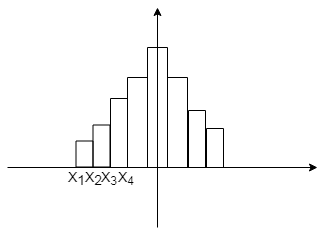
\includegraphics[scale=0.6]{pg47.png}\\

\begin{figure}[!h]
\begin{picture}(100,100)
\put(50,20){\vector(0, 3){80}}
\put(0, 20){\vector(4, 0){100}}
\put(55, 20){\line(0, 1){40}}
\put(55, 60){\line(-1, 0){10}}
\put(45, 20){\line(0, 1){40}}
\put(35, 20){\line(0, 1){30}}
\put(35, 50){\line(1, 0){10}}
\put(55, 50){\line(1, 0){10}}
\put(65, 20){\line(0, 1){30}}
\put(25, 45){\line(1, 0){10}}
\put(25, 20){\line(0, 1){25}}
\put(75, 20){\line(0, 1){20}}
\put(15, 20){\line(0, 1){15}}
\put(15, 35){\line(1, 0){10}}
\put(85, 20){\line(0, 1){10}}
\put(75, 30){\line(1, 0){10}}
\put(65, 40){\line(1, 0){10}}
\put(13, 10){\makebox(0, 0)   {$x_1$}}
\put(25, 10){\makebox(0, 0)   {$x_2$}}
\put(38, 10){\makebox(0, 0)   {$x_3$}}
\put(15, 20){\circle*{2}}
\put(25, 20){\circle*{2}}
\put(35, 20){\circle*{2}}
\end{picture}
\caption{Статистический ряд $x$}
\end{figure}
Для построения статистической функции распределения обычно приписывают $p_i^*$ середине $i$-го интервала $\frac{x_i + x_{i + 1}}{2} = x_i^*$. И дальше строят ступенчатую функцию для данного статистического ряда. Иногда строят не ступенчатую, а например функцию соединяя значения, соответствующие концам интервала\\
Можно ввести по аналогии с вероятностными -- статистические числовые характеристики. Однако, в большей степени они интересны не сами по себе, а той информацией, которую они содержат об измеряемой величине.
%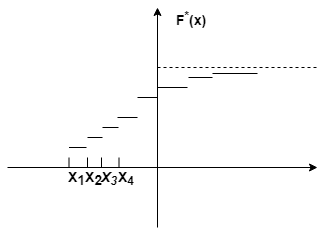
\includegraphics[scale=0.6]{pg47_2.png}\\
\begin{figure}[!h]

\begin{picture}(100,100)
\multiput(50,82)(4,0){13}{\line(1, 0){2}}
\put(33, 95){\makebox(0, 0)   {$F^*(x)$}}
\put(50, 0){\vector(0, 3){100}}
\put(10, 40){\circle*{2}}
\put(25, 40){\circle*{2}}
\put(40, 40){\circle*{2}}
\put(60, 40){\circle*{2}}
\put(73, 40){\circle*{2}}
\put(86, 40){\circle*{2}}
\put(99, 40){\circle*{2}}


\put(10, 50){\circle*{2}}
\put(25, 60){\circle*{2}}
\put(40, 65){\circle*{2}}
\put(60, 70){\circle*{2}}
\put(73, 73){\circle*{2}}
\put(86, 80){\circle*{2}}
\put(99, 81){\circle*{2}}


\put(25, 60){\line(15, 5){16}}
\put(10, 50){\line(15, 10){16}}
\put(40, 65){\line(20, 5){19}}
\put(60, 70){\line(13, 3){13}}
\put(73, 73){\line(13, 7){13}}
\put(86, 80){\line(13, 1){13}}

\put(10, 30){\makebox(0, 0)   {$x_1$}}
\put(25, 30){\makebox(0, 0)   {$x_2$}}
\put(40, 30){\makebox(0, 0)   {$x_3$}}
\put(60, 30){\makebox(0, 0)   {$x_4$}}
\put(75, 30){\makebox(0, 0)   {$x_5$}}
\put(89, 30){\makebox(0, 0)   {$x_6$}}
\put(102, 30){\makebox(0, 0)   {$x_7$}}

\put(0, 40){\vector(4, 0){120}}
\normalsize
\end{picture}
\caption{Статистическая функция распределения $F^*(x)$}
\end{figure}\\
\\
\begin{figure}[!h]
\begin{picture}(150,100)
\multiput(50,82)(4,0){13}{\line(1, 0){2}}
\put(33, 95){\makebox(0, 0)   {$\Large F^*(x)$} }
\put(50, 0){\vector(0, 3){100}}
\put(10, 40){\circle*{2}}
\put(25, 40){\circle*{2}}
\put(40, 40){\circle*{2}}
\put(60, 40){\circle*{2}}
\put(73, 40){\circle*{2}}
\put(86, 40){\circle*{2}}
\put(99, 40){\circle*{2}}
\put(10, 50){\circle*{2}}
\put(25, 60){\line(1, 0){16}}
\put(10, 50){\line(1, 0){16}}
\put(40, 65){\line(1, 0){20}}
\put(60, 70){\line(1, 0){13}}
\put(73, 73){\line(1, 0){13}}
\put(86, 80){\line(1, 0){12}}
\put(25, 60){\circle*{2}}
\put(40, 65){\circle*{2}}
\put(60, 70){\circle*{2}}
\put(73, 73){\circle*{2}}
\put(86, 80){\circle*{2}}
\put(99, 81){\circle*{2}}
\put(10, 30){\makebox(0, 0)   {$x_1$}}
\put(25, 30){\makebox(0, 0)   {$x_2$}}
\put(40, 30){\makebox(0, 0)   {$x_3$}}
\put(60, 30){\makebox(0, 0)   {$x_4$}}
\put(75, 30){\makebox(0, 0)   {$x_5$}}
\put(89, 30){\makebox(0, 0)   {$x_6$}}
\put(102, 30){\makebox(0, 0)   {$x_7$}}
\put(0, 40){\vector(4, 0){120}}
\end{picture}
\caption{Статистическая функция распределения $F^*(x)$ ступенчатого вида}
\end{figure}\\
%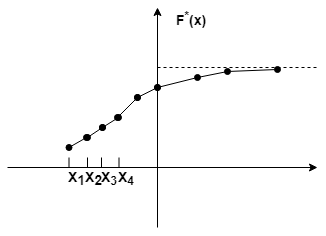
\includegraphics[scale=0.6]{pg47_3.png}\\
%страница 48
\subsection{Точечные оценки параметров распределения}
\noindent
Часто вид распределения известен заранее, а определить надо его параметры (например для нормального $m$ и $\sigma$), или закон распределения нас не интересует, а нужны лишь его числовые характеристики.  Если при этом после статистической обработки мы предлагаем для данного параметра в качестве приближения одно число, то это число называется точечной оценкой параметра. Пусть у случайной величины $X$ закон распределения содержит параметр $a$. Мы производим $n$ независимых измерений величины $X$ и получаем значения $X_1, X_2, $ . . . $,X_n$. Их можно рассматривать как $n$ экземпляров случайной величины $X$, то есть $n$ независимых случайных величин с тем же законом распределения. На основе $X_1, X_2, $ . . . $,X_n$ мы находим оценку â параметра a = â  = â$(X_1, X_2, \ .\ .\ . X_n)$ , то есть оценка это случайная величина. Её закон распределения зависит от закона распределения $X$ и от числа опытов. Какие оценки хороши?\\
\textit{\textbf{Определение}} \\
Оценка â называется состоятельной, если при $n \rightarrow \infty$ она сходится по вероятности к $a$\\
\textit{\textbf{Определение}} \\
Оценка â называется несмещённой, если её математическое ожидание равно a. $M($â$) = $ a. Это говорит об отсутствии систематических ошибок при оценивании.\\
\textit{\textbf{Определение}} \\
Несмещенная оценка называется эффективной, если её дисперсия минимальна по сравнению с другими оценками.
\begin{center}
$\textbf{Оценки математического ожидания и дисперсии}$
\end{center}
Пусть случайная величина $X$ имеет $M(X) = m$ и $D(X) = D$ ($M$ и $D$ неизвестны). $X_1, X_2, $ . . . $,X_n$ -- наблюдаемые величины $X$.\\
 $\hat{m} =  \cfrac{\displaystyle{\sum \limits_{i = 1}^{ n }}x_i}{n} $ \normalsize\\
Это состоятельная оценка так как по закону больших чисел, при $n \rightarrow \infty$  $\hat{m}$ сходится по вероятности к $m$. Оценка $\hat{m}$ несмещённая, так как \\$M(\hat{m}) =\cfrac{  \displaystyle{\sum \limits_{i = 1}^{n}} M(X_i)  }{n} = m$.\\ Дисперсия оценки: $D(\hat{m}) = \frac{1}{n^2} \displaystyle{\sum \limits_{i = 1}^{n}}D(X_i)	  = \frac{D}{n}$\\
Отсюда видно, зачем надо производить несколько измерений, а потом усреднять -- уменьшать дисперсию (точность увеличивается  в $\sqrt{n}$ раз).\\
%страница 49
Эффект оценки зависит от вида распределения. Если $X$ распределена нормально, то оценка $\hat{m}$ эфективна.  Для других законов это может не выполнятся. Если $n$
велико(практически $n>30$) и $x_i$ некоррелируют, то по центральной предельной теореме $\hat{m}$ подчиняется нормальному распределению со средним значением $m$ и среднеквадратичным отклонением $\sqrt{\frac{D}{n}}$\\
Оценка дисперсии.\\
Можно предположить: $ S^2 = \cfrac{ \displaystyle{\sum \limits_{i = 1}^{n}} (X_i - \hat{m})^2 }{\normalsize  n}$, $\hat{m} = \cfrac{ \displaystyle{\sum \limits_{i = 1}^{n}} x_i}{n}$\\
1)Оценка состоятельна\\
$S^2=\cfrac{ \displaystyle{\sum \limits_{i = 1}^{n}} (X_i)^2 }{n}- \hat{m}^2$\\
Это среднее  арифметическое $n$ наблюдений значений величины $X^2$. Он сходится по вероятности (по закону больших чисел) к $M(X^2) = \alpha_2(X)$. Второй член сходится по вероятности к $m^2$. То есть $S^2$ $\displaystyle{\underset{n \rightarrow \infty}{\rightarrow}} \alpha_2(x) - m^2 = D$ (по вероятности)\\
2)Оценка $S^2$ -- смещена.\\
$S^2$= $\cfrac{ \displaystyle{\sum \limits_{i = 1}^{n}}x_i^2 }{n} -  \displaystyle{ \left ( \frac{\sum \limits_{i = 1}^{n}x_i }{n} \right )^2 } = \frac{ \displaystyle{\sum \limits_{i = 1}^{n}}x_i^2 }{n}  - \frac{ \displaystyle{\sum \limits_{i = 1}^{n}}x_i^2 }{n^2} - 2 \frac{ \displaystyle{\sum \limits_{i < j}^{n}}x_ix_j }{n^2}  = \frac{n - 1}{n} \displaystyle{\sum \limits_{i = 1}^{n}}x_i^2  - 2 \frac{ \displaystyle{\sum \limits_{i < j}^{n}}x_ix_j }{n^2}  $  \\
$M(S^2) = \cfrac{n - 1}{n^2}  \displaystyle{\sum \limits_{i = 1}^{n}}M(X_i^2) - \frac{2}{n^2}  \displaystyle{\sum \limits_{i < j}^{}} M(X_iX_j)$\\
$S^2$ не зависит от выбора начала координат. Пусть начало координат в точкe $m$. Тогда $M(X_i^2) = M(\hat{X}_i^2) =D$, $ \displaystyle{\sum \limits _{i=1} ^ {n}} M(X_i^2) = nD$, $M(X_iX_j) = M(\hat{X_i}\hat{X_j}) = K_{ij} = 0$. (так как опыты независимы, следовательно некоррелируют).\\
Значит, $M(S^2) = \frac{n - 1}{n} D \neq D$\\
\\
Что бы оценка стала несмещённой, ее надо умножить на $\frac{n}{n - 1}$.\\
$\hat{D} = \cfrac{\displaystyle{\sum \limits _{i = 1}^{n}( (x_i - \hat{m})^2 }}{n - 1}$ -- несмещённая оценка. $ \displaystyle{\left ( или \hat{D} = \frac{\sum \limits _{i = 1}^{n} x_i^2}{n - 1} - \hat{m^2} \frac{n}{n - 1}\right )}$\\
При больших значениях $n$ -- $S^2$ и $\hat{D}$ различаются мало.\\ При известном математическом ожидании ($m$) несмещённая оценка дисперсии:$\hat{D} = \cfrac{1}{n} \displaystyle{\sum \limits_{i=1}^{n}(x_i - m)^2}$.\\ (То есть $\cfrac{1}{n - 1}$ происходит из-за того, что была оценкой $\hat{m}$, а не $m$).\\
$ \displaystyle{M \left( \frac{1}{n} \sum \limits_{i = 1}^{n} (X_i - m)^2 \right) = \frac{1}{n} \displaystyle{\sum \limits_{i = 1}^{n}} M((X_i - m)^2) = \frac{1}{n} \displaystyle{\sum \limits_{i = 1}^{n}}  D = D}$,
{то есть она несмещённая.}\\
%страница 50
\textbf{Пример}\\
Для определения точности измерительного прибора (лазерного дальномера) систематическая ошибка которого практически равна нулю, было произведено 5 независимых измерений.\\
$x_i$  = 2781 метра, 2836 метра, 2807 метра, 2763 метра, 2858 метра. Определить несмещённую оценку дисперсий ошибок  измерительного прибора, если значение измеряемой величины:\\
a)известно и равно 2800 м\\
б) неизвестно\\
\textbf{Решение}\\
a)$\hat{D}(X) = \frac{1}{n} \displaystyle{\sum \limits_{j = 1}^{n}}(x_j - m)^2 = \frac{6439}{5} = 1287.8$ квадратных метров\\
b)$\hat{m} = \frac{1}{n} \displaystyle{\sum \limits_{j = 1}^{n}}(x_j)= 2809$  метров\\
$\hat{D}(X) = \frac{1}{n} \displaystyle{\sum \limits_{j = 1}^{n}}(x_j - \hat{m})^2 = \frac{6034}{4} = 1508.5$ квадратных метров\\
%страница 51
\subsection{Интервальные оценки параметров}
\noindent
Если для оценки параметра предлагается интервал, в который его значение попадает с заданой вероятностью, то такая оценка называется интервальной.\\
\textit{\textbf{Определение}} \\
Доверительным интервалом называется интервал, который с заданой доверительной вероятностью $\beta$ накрывает оцениваемый параметр $a$.\\
Оценка $\hat{a}$ случайна, и поэтому замена $a$ на $\hat{a}$ может привести к ошибкам. Интервалы оценки вводятся для того, что бы можно было судить о надёжности оценки. Для симметричного доверительного интервала его ширина $2\varepsilon$ определяется условием: $P(\abs{\hat{a} - a} \leq \varepsilon) = \beta$\\
Доверительный интервал: $(\hat{a} - \varepsilon, \hat{a} + \varepsilon) = I_\beta$\\
\begin{figure}[!h]
\begin{picture}(200,60)
\qbezier(20,30)(10,20)(20,10)
\qbezier(170,30)(180,20)(170,10)
\put(10, 20){\line(1,0 ){180}}
\put(100, 20){\line(0,-1 ){3}}
\put(60, 18){\line(1,1 ){4}}
\put(60, 22){\line(1,-1 ){4}}
\put(95, 8){\makebox(10, 0){$\hat{a}$}}
\put(58, 26){\makebox(10, 0){$a$}}
\put(15, 0){\makebox(10, 0){$\hat{a} - \varepsilon$}}
\put(170, 0){\makebox(10, 0){$\hat{a} + \varepsilon$}}
\end{picture}
\caption{Доверительный интервал}
\end{figure}\\
%сюда картинку
\textbf{Замечание\ } \\
Здесь $a$ не является случайным, случаен интервал, положение которого задаётся случайным положением $\hat{a}$.
$ \hat{a} - \varepsilon$ и $\hat{a} + \varepsilon$ -- доверительные границы.\\
Пусть проведено  $n$ измерений величины $X$ (с $M(X)=m$, $D(X) = D$\\
 Оценки:  $\hat{m}= \frac{1}{n} \displaystyle{\sum\limits_{i=1} ^ {n}} X_i$, $\hat{D} = \frac{1}{n - 1}$  $\displaystyle{\sum \limits_{i=1} ^ {n}} (x_i - \hat{m})^2$\\
Построим доверительный интервал $I_\beta$ для математического ожидания $\hat{m}$ -- сумма $n$ независимых одинаково распределенных случайных величин $X_i$. \\
По центральной предельной теореме при большом $n$ закон распределения $\hat{m}$ близок к нормальному с математическим ожиданием $m$ и дисперсией $\frac{D}{n}$. Пусть дисперсия $D$ известна. Найдем доверительные границы $P(\abs{\hat{m} - m} < \varepsilon_\beta) = \beta$. 
Так как $\hat{m}$ распределен нормально с $\sigma_{\hat{m}} = \sqrt{\frac{D}{n}}$\\
$\beta = P(\abs{\hat{m} - m} < \varepsilon_\beta)$
$ = 2\Phi^*(\frac{\varepsilon_\beta}{\sigma_{\hat{m}}}) - 1$.\\
$\Phi^*(x) = \frac{1}{\sqrt{2\pi}} \displaystyle{\int \limits _{-\infty} ^ {x}} e^{-\frac{t^2}{2}} dt$\\
Находим $t_\beta$ по таблице функции $\Phi^*(x)$: $2\Phi^*(t_\beta) - 1 = \beta$\\
$\Phi^*(t_\beta) = \frac{\beta + 1}{2}$\\
Тогда, $\varepsilon_\beta = t_{\beta} \sqrt{\frac{D}{n}}$\\
Доверительный интервал: $(\hat{m} - t_\beta \sqrt{\frac{D}{n}}, \hat{m} + t_\beta \sqrt{\frac{D}{n}})$\\
%страница 52
Если $D$ неизвестна, то в качестве её ориeнтировочного значения  можно взять $\hat{D}$ и положить приближенно $\sigma_{\hat{m}} = \sqrt{ \frac{\hat{D}}{n} }$\\
Но при этой замене возникает дополнительная ошибка. Для точного определения доверительного интервала необходимо знать вид знать вид закона распределения $X$.
Пусть,например, $X$ 
распределено по нормальному закону. Произведено $n$ измерений. $\hat{m} = \frac{1}{n} \displaystyle{\sum \limits_{i=1} ^ {n} } X_i$, $\hat{D} = \frac{1}{n - 1} \displaystyle{\sum \limits_{i=1} ^ {n} } (x_i - \hat{m})^2$.\\
Оказывается, что величина $T = \sqrt{n} \frac{\hat{m} - m}{\sqrt{\hat{D}}}$ подчиняется закону распределения Стьюдента с $(n-1)$ степенями свободы, не зависящих от неизвестных параметров $m$ и $D$, плотность которого $S_{n-1} = \frac{\Gamma(\frac{n}{2})}{\sqrt{(n-1)\pi}}(1 + \frac{t^2}{n - 1})^{-\frac{n}{2}}$, \\где $\Gamma (x)$ -- гамма-функция Эйлера.( $\Gamma (x) = \displaystyle{\int \limits_{0} ^ {\infty} } u^{x - 1} e ^{-u}du$.)\\
Найдем доверительный интервал соответствующий вероятности $\beta$: \\
$ P(\abs{\hat{m} - m} < \varepsilon) = \beta$ $\Leftrightarrow$ $\displaystyle { P\left (\frac{\sqrt{n} \abs{\hat{m} - m}}{\sqrt{\hat{D}}} < \frac{\varepsilon_\beta}{\sqrt{\frac{\hat{D}}{n}}}\right ) = \beta}$ $\Leftrightarrow$  $\displaystyle { P\left (\abs{T} < \frac{\varepsilon_\beta}{\sqrt{\frac{\hat{D}}{n}}} \right )}= \beta $.\\
Найдем  $t_\beta$ из : $P(\abs{T} < t_\beta) = \beta$\\
$P(\abs{T} < t_\beta) = \displaystyle{\int \limits_{-t_{\beta}}^{t_{\beta}}} S_{n-1}(t) dt = \beta$.\\
(Замечание: $S_{n-1}$ -- четная функция, поэтому  $\displaystyle{\int \limits_{-t_{\beta}}^{t_{\beta}}} S_{n-1}(t) dt =  2\displaystyle{\int \limits_{0}^{t_{\beta}}} S_{n-1}(t) dt$)\\
$t_\beta(n)$ называется коэффициент Стьюдента. Для них существуют таблицы.)\\
Определив по таблице $t_\beta$ находим полуширину доверительного интервала $\varepsilon_\beta = t_\beta \sqrt{\frac{\hat{D}}{n}}$. Доверительный интервал при неизвестной дисперсии: $(\hat{m} - t_\beta \sqrt{\frac{\hat{D}}{n}}, \hat{m} + t_\beta \sqrt{\frac{\hat{D}}{n}} )$, $t_\beta$  -- коэффициент Стьюдента при $(n-1)$ степени свободы.\\
%странциа 53
\textbf{Пример}\\
Оцениваем средний рост мужчины. Выборка $10$ человек. Результат: $160,\ 160,$\\
 $\ 167,\ 170,\ 173,\ 176,\ 178,\ 178,\ 181,\ 181$.\\
Найдем $\hat{m} = 172.4$. $\hat{D} = \frac{1}{9} \displaystyle{\sum \limits _{x_i = 1}^{10}} (x_i - 172.4)^2 = 62.9$\\
$\sqrt{\frac{\hat{D}}{n}} = 2.51$. Если $\beta = 0.95$, то $t_\beta(9) = 1.83$. $\varepsilon_\beta = 1.83 \cdot 2.51 \approx 4.6$ , то есть $m=172.4 \pm 4.6$ с вероятностью $0.95$.\\
\textbf{Замечание\ } \\
Физики обычно предпочитают приводить результат $\pm$ одно среднее квадратичное отклонение. Из таблиц распределения Стьюдента следует, что доверительный интервал полушириной в одно среднее  квадратичное отклонение содержит истинный результат с вероятностью всего $0.66$.
%страница 54
\begin{center}
$\textbf{Доверительный интервал для дисперсии }$
\end{center}
$\hat{D}$ -- сумма $n$ случайных величин вида: $\frac{(x_i - \hat{m})}{n - 1}$. Они зависимы, так как $\hat{m}$ зависит от всех $X_i$. Но при  $n \rightarrow \infty$ распределение их суммы приближается к нормальному. При $n \in (20, 30)$ его уже приближенно можно считать нормальным. Опишем 
приближённый способ построения доверительного интервала. Найдем характеристики этого приближенного нормального распределения. $M(\hat{D}) = D$. (оценка $\hat{D}$ несмещенна.)\\ $D(\hat{D}) = \frac{1}{n}\mu_4 - \frac{n-3}{n(n-1)}D^2$\\
Вместо $D$ можно взять $\tilde{D}$. Брать вместо $\mu_4$ его оценку $\frac{1}{n}\displaystyle{\sum \limits _{i=1} ^ {n} } (x_i - \hat{m})^4$ плохо, так как при небольшом $n$ ошибка будет велика. Если известен закон распределения $X$, то $\mu_4$ можно выразить через $D$. Для нормального распределения $X$ : $\mu_4 = 3D^2$, следовательно, $D(\hat{D}) = \frac{3}{n} D^2 - \frac{n - 3}{n(n-1)}D^2 = \frac{2}{n - 1}D^2 \approx \frac{2}{n - 1} \hat{D}^2 $. $\sigma_{\hat{D}} = \sqrt{\frac{2}{n - 1}} \hat{D}$. Пусть доверительная вероятность $\beta$. Найдем $t_{\beta}$: $\Phi^*(t_{\beta}) = \frac{\beta + 1}{2}$, по таблице доверительного интервала для дисперсии: $(\hat{D} - t_\beta \sigma_{\hat{D}}, \hat{D} + t_\beta \sigma_{\hat{D}})$\\
\begin{center}
$\textbf{Точное построение доверительного интервала для дисперсии}$
\end{center}
Известно, что $V = \frac{(n-1)\hat{D}}{D}$ имеет распределение $\chi^2$ c $(n-1)$ степеней свободы, плотность которой:\\
\noindent
\begin{equation*} 
K_{n - 1}(V)=
 \begin{cases}
   0 ,\ \ \  V < 0\\
	\\
   \frac{1}{  2 ^{ { \frac{n - 1}{2}  }}  \Gamma(\frac{n - 1}{2})} V^{\frac{n - 1}{2} - 1}e^{-\frac{V}{2}}    , \ \ \ V > 0\\
 \end{cases}
\end{equation*}\\
\begin{figure}[!h]
\begin{tikzpicture}
[declare function={
            gamma(\x)= 0.25*\x*\x*exp(-0.5*\x);
    }
]
   \begin{axis}[ xmin = 0, xmax=0.5, ymin=0, ymax=0.5,
     ticks=none,
     at={(0,0.03\linewidth)},
     axis y line=middle,
     axis x line=middle,
     y label style={at={(axis description cs:.1,1)},anchor=south },
%y label style={ticks=none,at={(axis description cs:0.2,10)},rotate=270,anchor=south},
     axis line style={->},
     xlabel=$x$, ylabel=$K_{n-1}(V)$,
     scale=0.6]
     %\addplot[domain=-pi/2:pi/2,samples=200,black,pattern=north east lines]{pow(deg(x), 3)};
     \node[label={below :{$\alpha$}},circle,fill,inner sep=2pt] at (axis cs:-pi/2 + 0.30,0) {};
     \node[label={below:{$\beta$}},circle,fill,inner sep=2pt] at (axis cs:pi/2 - 0.30,0) {};
    % \addplot[blue, samples=100, smooth, unbounded coords=discard,domain=0.00001:9] {abs(x)^(1/3)};
     \addplot[domain=0.00001:pi/2,samples=200,black]{deg(x)^(2) * 2.17^(- deg(x) / 2)/ 12};
      \addplot[domain=0.00001:pi/60,samples=200,black,pattern=north east lines]{deg(x)^(2) * 2.17^(- deg(x) / 2)/ 12}\closedcycle;	
       \addplot[domain=pi/15:0.5,samples=200,black,pattern=north east lines]{deg(x)^(2) * 2.17^(- deg(x) / 2)/ 12}\closedcycle;
\end{axis}
   \draw [<-] (0.5,0.2) -- (0.7,0.2);	
    \draw [->] (1.3,0.2) -- (1.7,0.2);
    \node [black, right] at (0.7,0.2) {$l_{\beta}$};
\end{tikzpicture}\\
\caption{График $K_{n - 1}(V)$ }
\end{figure}\\
Будем выбирать интервал $l_\beta$ так, чтобы вероятности выхода $V$ за пределы  $l_\beta$ влево и вправо были одинаковы  и равны.\\
$\frac{\alpha}{2} = \frac{1 - \beta}{2}$. Распределение $\chi^2$ затабулировано. Здесь приведем числа $\chi^2$ такие, что $P(V> \chi^2) = p$, $r$ -- число степеней свободы.
$(r = n - 1)$.\\
%страница 55
Зафиксируем $r = n - 1$ и найдем по таблице два значения  $\chi^2$, одно соответствует $p_1 = \frac{\alpha}{2}$, другое $p_2 = 1 - \frac{\alpha}{2}$. Обозначим их $\chi_1^2$ и  $\chi_2^2$. Интервал $l_\beta$ = $ (\chi_2^2$, $\chi_1^2)$.\\
Доверительный интервал для дисперсии $P(D_1 < D < D_2) = \beta$ -- он будет тогда, когда $V = \frac{(n - 1) \hat{D}}{D}$ попадет в $l_\beta$.\\
Если $V < \chi_1^2$, то $\frac{(n - 1) \hat{D}}{D}M  < \chi_1^2$ следовательно $\frac{(n - 1) \hat{D}}{\chi_1^2} < D$.\\
Если $V > \chi_2^2$, то $\frac{(n - 1) \hat{D}}{D}M  > \chi_2^2$ следовательно $\frac{(n - 1) \hat{D}}{\chi_2^2} > D$.\\
То есть доверительный интервал для дисперсии: $\displaystyle{\left(\frac{(n - 1) \hat{D}}{\chi_1^2}, \frac{(n - 1) \hat{D}}{\chi_2^2}\right)}$
%страница 56
\subsection{Оценки числовых характеристик случайных величин}
Система $(X, Y)$. Результат $n$ опытов $(x_1, y_1)$, . . . $(x_n, y_n)$.\\
Несмещенные оценки:\\
$\hat{m}_x= \frac{1}{n} \displaystyle{\sum\limits_{i = 1} ^{n}} x_i$,  $\hat{m}_y= \frac{1}{n} \displaystyle{\sum\limits_{i = 1} ^{n}} y_i$,\\
$\hat{D}_x = \frac{1}{n - 1} \displaystyle{\sum\limits_{i = 1} ^{n}} (x_i - \hat{m}_x)^2$, 
$\hat{D}_y  = \frac{1}{n - 1} \displaystyle{\sum\limits_{i = 1} ^{n}} (y_i - \hat{m}_y)^2$.\\
$\hat{K}_{XY} = \frac{1}{n - 1} \displaystyle{\sum\limits_{i = 1} ^{n}} (x_i - \hat{m}_x) (y_i - \hat{m}_y)$ 
%страница 57
\subsection{Проверка гипотез}
Рассмотрим задачу проверки опытных данных заданому закону распределения.
\begin{center}\textbf{Критерий согласия $\chi^2$ Пирсона по измерению $X$}\end{center}
Пусть в результате опытов (независимых) получены результаты, которые сведены в статистический ряд. ($p_i^*$ -- частоты)\\
\begin{tabular}[b]{ | l |  l | l |    }
\hline
$x_1$, $x_2$ &... &$ x_k$,$x_{k+1}$\\
\hline
$p^*_1$&...&$p^*_k$\\
\hline
$p_1$& ... &$p_k$\\
\hline
\end{tabular}\\
Мы предполагаем, что $X$ распределена по некоторому "теоретическому"$\ $ закону. На основании его вычисляем теоретические вероятности попадания случайной величины в $(x_1,x_2),$ . . . $,(x_k, x_{k+1})$. Мера расхождения $U = \displaystyle{\sum \limits_{i = 1} ^ {k}} c_i(p_i^* - p_i)^2$. 
"Весовые"\  коэфициенты надо выбирать обратно пропорционально  вероятностям, так как одно и то же значение $p^*-p$ более значимо  если само $p_i$ мало. Возьмем $c_i=\frac{n}{p_i}$. Тогда $U$ будет распределено по "закону $\chi^2$".\\
\textbf{Замечание\ } \\
Пусть $X_i$ -- независимые случайные величины, распределенные, по нормальному закону с $M(X_i) = 0$, $\sigma_{x_i} = 1$. Тогда величина $U = \displaystyle{\sum \limits_{i  = 1}^{r}} x_i^2$ распределена по закону c $\chi^2$ с $r$ степенями свободы. У нас: $U = \chi^2 = \displaystyle{\sum \limits_{i = 1}^{k}} \frac{n(p_i^* - p_i)^2}{p_i}$ = $\displaystyle{\sum \limits_{i = 1}^{k}} \frac{(m_i - np_i)^2}{n p_i}$,  так как $p_i^* = \frac{m_i}{n}$.\\
Число степеней свободы $r$ равно числу разрядов $k$ минус число независимых условий, наложенных на частоты $p_i^*$. Одно из таких условий, которое всегда накладывается : $\displaystyle{\sum \limits _{i = 1} ^ {k}} p_i^* = 1$\\
Если все параметры "теоретического"\ распределения заранее известны, то больше условий нет. Если эти параметры мы оцениваем из результатов опытов, то добавляется еще условие, например $\displaystyle{\sum \limits_{i = 1} ^ {k}} x_i^* p_i^* = m_x$, $\displaystyle{\sum \limits_{i = 1} ^ {k}}( x_i^* - \hat{m_x} )^2 p_i^* = D_x$, и соответственно уменьшается число степеней свободы.\\
%страница 58
Рассмотрим на примере действие критерия $\chi^2$.\\
\textbf{Пример}\\
$20$ лет собирали сведения о количестве офицеров русской армии, погибших в результате гибели под ними коня. (на основании ежегодных докладов 10 армейских корпусов , то есть 200 донесений).\\
Пусть $X$ -- число погибших в одном корпусе за год.\\
\begin{tabular}[b]{ | l |  l | l |  l |   l |   l |   l |   l |     }
\hline
Количество погибших, $x_i$ &0&1&2&3&4&5& всего\\
\hline
Количество доненесений $m_i$ &109&65&22&3&1&0&200\\
с указанием $x_i$ погибших& &  & & & & &\\
\hline
Ожидаемая (по пуассону)& 108.7&66.3&20.2&4.1&0.6&0.07&200\\
частота $p_i$& & & & & & & \\
\hline
\end{tabular}\\
Полное число погибших: $0\cdot 109 + 1 \cdot 65 + 2 \cdot 22 + 3 \cdot 3 + 4 \cdot 1=122$.\\
Среднее число погибших: $\frac{122}{200} = 0.61$. Проверим гипотезу о том, что эти данные описывают распределение Пуассона: $P(x = x_i) = p_i = \frac{\mu^ie^{-\mu}}{i!}$. Для определения $p_i$ надо оценить одним параметром $\mu$. В качестве $\mu$ возьмем $\hat{\mu} = 0.61$. $np_i$ приведен в третьей строке. Так как ожидаемые частоты для $x_i > 2$ малы, объединим их $U = \chi^2 = \displaystyle{\sum } \frac{(m_i - np_i)^2}{np_i} = \frac{(0.3)^2}{108.7} + \frac{(1.3)^2}{66.3} + \frac{(1.8)^2}{20.2} + \frac{(0.8)^2}{4.8} = 0.32$. \\
\begin{tabular}[b]{ | l |  l | l |  l |   l |     }
\hline
$x_i$&0&1&2&$\geq 3$\\
\hline
$m_i$&109&65&22&4\\
\hline
$np_i$&108.7&66.3&20.2&4.8\\
\hline
\end{tabular}\\
Есть 2 линейки соотношений, связывающие частоты: $\displaystyle{\sum\limits} m_i = 200$ и $\displaystyle{\sum\limits} x_im_i = 122 = \hat{\mu}$.\\
То есть число степеней свободы : $r = 4 - 1 - 1 = 2$. То есть $U$ распределено примерно  по закону $\chi^2$ с двумя степенями свободы. $U$ распределено примерно по закону $\chi^2$ с двумя степенями свободы.\\
Из таблицы распределения $\chi^2$ c $r=2$ находим, что с вероятностью $0.95$ $\chi^2$ должно лежать в интервале от $0$ до $6.0$ так  как наше значение  $0.32$ попадает в этот незначимый интервал, то проверяемая гипотеза не отвергается.
В таблице указана вероятность $p$ того, что $\chi^2 \geq \chi^2_p$ при  числе степеней свободы $r$.
Если бы мы получили для $\chi^2$ значение $6.1$ или больше, то должны были бы считать  его значимым, так как если проверяемая гипотеза верна, то такие значения $\chi^2$ может принимать с вероятностью не более $0.05$. $0.05$ называется уровнем значимости.
Обычно, схема действий такая: По экспериментальным данным составляется функция $U$ и на основе "нулевой гипотезы" $H$ вычисляется её распределение. Затем проверяют, как изменится $U$, если гипотезы $H$ неверна (верна $\overline{H}$).
%страница 59
Обычно $U$ в этом случае намного больше. На рисунке показано два распределения величины $U$, соответствующие двум конкурирующим гипотезам $H(a)$ и $\hat{H}(\hat{a})$. Если из опыта получилось большое значение $U$, то можно сказать, то либо справедлива гипотеза $H$,но произошло чрезвычайно маловероятное событие,либо более правдоподобна гипотеза $\overline{H}$. Если оставаться в рамках одной гипотезы, то результат следует признать значимым в том смысле, что он выходит за рамки обычных статистических ошибок.\\
\newpage
\begin{figure}[!h]
\begin{tikzpicture}
[declare function={
            gamma(\x)= 0.25*\x*\x*exp(-0.5*\x);
    }
]
   \begin{axis}[ xmin = 0, xmax=0.5, ymin=0, ymax=1,
     ticks=none,
     at={(0,0.1\linewidth)},
     axis y line=middle,
     axis x line=middle,
     y label style={at={(axis description cs:.1,1)},anchor=south },
      x  label style={at={(axis description cs:1.01,.01)},anchor=south },
%y label style={ticks=none,at={(axis description cs:0.2,10)},rotate=270,anchor=south},
     axis line style={->},
     xlabel=$x$, ylabel=$K_{n-1}(V)$,
     scale=1]
 % \addplot[domain=0.00001:pi/2,samples=200,black]{deg(x)^(2) * 2.17^(- deg(x) / 2)/ 12};
      \addplot[domain=0.00001:pi/2,samples=200,black]{(deg(x + 0.25))^(2) * 2.17^(- (deg(x + 0.25) ) / 2)};
  \addplot[domain=0.00001:0.5,samples=200,black]{(deg(0.52 - x)/2)^(2) * 2.17^(- (deg(0.52 - x)/2) / 2)/ 12};
 \addplot[domain=0.00001:0.15,samples=200,black,pattern=north east lines]{(deg(0.52 - x)/2)^(2) * 2.17^(- (deg(0.52 - x)/2) / 2)/ 12}\closedcycle;
      \addplot[domain=0.15:pi/2,samples=200,black,pattern=north west lines]{(deg(x + 0.25))^(2) * 2.17^(- (deg(x + 0.25) ) / 2)}\closedcycle;
\end{axis}
  \node [black, right] at (1.5,1) {$u_{\alpha}$};
 \node [black, right] at (0.5,4) {$a$};
 \node [black, right] at (2.2,3) {$b$};
  \node [black, left] at (0.5,2.3) {$\beta$};
  \node [black, right] at (3.05,2.3657) {$\alpha$};
 \draw [->] (0.5,2.3) -- (0.6,2.1);
 \draw [->] (3.2,2.3) -- (3.0,1.7);
\end{tikzpicture}
\caption{Сравнение конкурирующих гипотез}
\end{figure}
\noindent
\textit{\textbf{Определение}}\\
Отвергая нулевую гипотезу $H$, когда она справедлива, мы совершаем ошибку первого рода. Принимая нулевую гипотезу $H$, когда справедлива конкурирующая гипотеза 
 $\overline{H}$, мы совершаем ошибку второго рода. Вероятность ошибки первого рода называется уровнем значимости ($\alpha$). Если вероятность ошибки второго рода равна $\beta$, то $1 - \beta$ называют мощностью критерия.\\
Часто возможен компромисс между уровнем значимости и мощностью критерия. Если $U>U_{\alpha}$, мы отвергаем $H$ и принимаем $\overline{H}$, если $U>U_{\alpha}$ -- наоборот.
%страница 60
\subsection{Метод моментов}
\noindent
Пусть функция распределения случайной величины $X$ зависит от $k$ параметров $a_1, a_2$ . . . $a_k$. Надо выбрать оценки этих параметров по результатом $n$ опытов. Теоретические моменты $(M(X), D(X), ... \mu_k(x))$ являются функциями от этих параметров. По результатам опытов находим оценки моментов  $\hat{M}(X),\hat{D}(X), ... \hat{\mu_k}(x)$.
Оценки параметров $a_1, a_2$. . . $a_k$ находим решая систему уравнений:\\
\begin{equation*} 
 \begin{cases}
  m_x = \hat{m}_x\\
  D(X) (a_1, ... a_k) = \hat{D}(X)\\
  ....\\
 \mu_k(x) (a_1, ... a_k) = \hat{\mu}_k(X)
 \end{cases}
\end{equation*}
\textbf{Пример}\\
Найти точечные оценки параметров $a, b$ равномерно распределенных в интервале $(a, b)$ по результатам $n$ опытов. По результатам $n$ опытов находим $\hat{m_x} = \overline{x}$, и $\hat{D}(X) = \hat{\sigma_x^2}$.\\
Теоретические моменты:\\
$M(X) = \frac{a + b}{2} = \overline{X}$\\
$D(X) = \frac{(b-a)^2}{12} = \hat{D}_x = \hat{\sigma}_x^2$.\\
Решая эту систему, находим оценки для $a$ и $b$: $\hat{a} = \overline{X} - \hat{\sigma}_{x} \sqrt{3}$,  $\hat{b} = \overline{X} + \hat{\sigma}_x \sqrt{3}$.\\
\textbf{Замечание\ } \\
Об ошибке прибора при  измерении. Если в паспорте прибора задан гарантированный его производителем интервал $\pm \Delta$, из которого не выходят предельные отклонения (ошибки).  Тогда дисперсия ошибки $D = \frac{\Delta^2}{3}$. Если задан класс точности прибора (a), то $\Delta = \frac{a \cdot b}{100}$, где b -- максимальное значение шкалы прибора.\\
%страница 61
\subsection{Принцип максимального правдоподобия}
\noindent
Пусть есть урна, в которой неизвестная смесь черных и белых шаров.\\ Вероятность вытянуть белый шар -- $p$, может принимать любое значение от $0$ до $1$ .\\ 
Хотим изменить $p$, вынимая шар из урны. Пусть мы вытащили шар $n$ раз (с возвращением) и белый шар оказался в $r$ случаях. Вероятность этого события $l(p) = C^r_n p^r (1-p)^{n - r} = l(p|r)$ эта функция при неизвестном $r$ (и $n$) и неизвестном $p$ называется функцией правдоподобия. Выбираем то значение $p$, которое с наибольшей  вероятностью приводит к наблюдаемому значению $r$. Когда параметр $p$ дискретен, надо вычислить для разных $p$ функцию правдоподобия  и выбрать то $p$, при котором функция правдоподобия максимальна.  Если $p$ непрерывен, то можно искать максимум с помощью дифференцирования: $\frac{dl}{dp} = C^r_n (rp^{r - 1}(1-p)^{n - r} - (n - r) p ^ r  (1-p) ^{n - r - 1}) = 0$\\
$r - rp - np - rp = 0$, $p = \frac{r}{n}$.\\
\textit{\textbf{Определение}}\\
Логарифмическая функция правдоподобия: \\$L(p|r) = \ln l(p|r) = r \ln p + (n-r) \ln (1-p)$. (здесь отброшено постоянное слагаемое, а в $l(a|r)$ -- постоянный множитель, который не влияет на максимум.)\\
$L(p|r)$ имеет максимум при том же значении $p$, что и $l(p|r)$.\\
Более общий случай:\\
%страница 62
Пусть $X$ -- дискретная случайная величина со значениями $x_1$ . . . $x_l$ и\\ $P(X=x_j; \theta) = p_j(\theta)$. $\theta = (\theta_1, $ . . .$,\theta_k)$ -- неизвестные параметры. Пусть $m_1, \ .\ .\ .,m_l$ -- число появлений значений $x_1, \ .\ .\ x_l$ в выборке $X_1, X_2, \ .\ .\ . X_n$. Тогда функция правдоподобия  значений $l(\theta | x_1, x_2, \ .\ .\ , x_n) = p_1^{m_1}(\theta) \cdot p_2^m(\theta) \cdot . \ .\ .\ p_l^{m_l}(\theta)$. $ L(\theta | x_1, x_2, \ .\ .\ , x_n) =\ln l (\theta | x_1, x_2, \ .\ .\ , x_n) $\\
Пусть случайная величина $X$ имеет непрерывное распределение с плотностью $f(x|\theta)$, $\theta$ -- единственный параметр. Плотность вероятности выборки из $n$ измерений ($n$ независимых случайных величин):\\
$\displaystyle{\prod_{i = 1} ^ n} f(x_i|\theta) = l(\theta|x1,x_2,\ .\ .\ ,x_n)$\\
Логарифмическая функция правдоподобия: $L(\theta|x_1,\ .\ .\ . x_n) = \displaystyle{\sum \limits_{i = 1} ^ {n}} \ln f(x_i|\theta)$\\
Если параметров несколько, то $\theta = (\theta_1, \theta_2, \ .\ .\ . ,\theta_k)$. Параметры выбираются из условия максимума функции $l$ (или $L$)\\
\textbf{Пример}\\ 
$f(x|m, \sigma^2) = \frac{1}{\sqrt{2\pi\sigma^2}} e^{-\frac{(x_i - m)^2}{2\sigma^2}}$\\
$l(\mu, \sigma^2|x_1, \ .\ .\ ., x_n) = (\sigma^2)^{-\frac{n}{2}}e^{\displaystyle{\cfrac{\sum \limits_{i = 1}^{n}(x_i - m)^2}{2\sigma^2}} }$\\
$L(\mu, \sigma^2|x_1, \ .\ .\ ., x_n) = - \frac{n}{2} ln \sigma^2 - \displaystyle{\sum \limits_{i = 1}^{n}}(x_i - m)^2\frac{(x_i - m)^2}{2\sigma^2}$\\
$\frac{\partial L}{\partial m} = 0, \frac{\partial L}{\partial \sigma^2} = 0$\\
Отсюда находим $\hat{m}, \hat{\sigma}^2$\\
$\frac{\partial L}{\partial m} = \frac{1}{\sigma^2} \displaystyle{\sum \limits _{i = 1} ^ {n} } (x_i - \hat{m}) = 0$, следовательно $\hat{m} = \overline{x}$\\
$\frac{\partial L}{\partial \sigma^2} = -\frac{n}{2} \frac{1}{\hat{\sigma}}^2 + \frac{1}{2\hat{\sigma}^2}  \displaystyle{\sum \limits _{i = 1} ^ {n} } (x_i - m)^2 = 0$, следовательно 
$\hat{\sigma}^2 = \frac{1}{n}  \displaystyle{\sum \limits _{i = 1} ^ {n} } (x_i - \overline{x})^2$\\
То есть тут оказывается смещённая оценка дисперсии.
%страница 63
\subsection{Метод наименьших квадратов}
\noindent
Пусть в эксперименте определяется зависимость величины $Y$ от величины $X$. Надо найти функцию $Y=\varphi(x)$ по экспериментальным данным. Часто вид $\varphi(x)$ известен (например прямая или парабола), а надо найти параметры этой кривой. Пусть истинная зависимость $Y = \varphi(x)$. Результат опыта $Y_i$ -- случайная величина, распределённая по нормальному закону с $M(Y_i)=\varphi(x_i)$ и $\sigma_{y_i} = \sigma_i$. Пусть все $\sigma_i = \sigma$. (Точность измерения везде одинакова)\\
Плотность $y_i$ : $f_i(y_i) = \frac{1}{\sigma \sqrt{2\pi}} e^{-\frac{(y_i - \varphi(x_i))^2}{2\sigma^2}}$.\\
Составим функцию правдоподобия  $Ce^{-\frac{1}{2\sigma^2}\displaystyle{\sum \limits_{i = 1}^{n}} (y_i - \varphi(x_i))^2}$, где $C$ -- константа зависящая от $\sigma$ и $n$.\\
Максимум функции правдоподобия достигается тогда, когда $\frac{1}{2\sigma^2}\displaystyle{\sum \limits_{i = 1}^{n}} (y_i-\varphi(x_i))^2$--\\-- минимально, то есть, что бы данная совокупность наблюдений $y_1, y_2,\ .\ .\ .y_n$ была наивероятнейшей, надо выбирать функцию $\varphi(x)$ так, что бы сумма квадратов отклонений наблюдаемых значений $y_i$ от $\varphi(x_i)$ была минимальной.\\
 ($\displaystyle{\sum \limits_{i = 1}^{n}} (y_i - \varphi(x_i))^2 = min$)\\
Пусть функция $\varphi$ зависит от параметров $a$, $b$, . . . : $y = \varphi(x, a, b, c, \ .\ .\ .)$\\
Параметры выбираются из условия $\displaystyle{\sum \limits_{i = 1}^{n}} (y_i - \varphi(x, a, b, c, \ .\ .\ .))^2$ -- минимально.\\
Условие минимума: производные по $a,\ b,\ c\ ...=\ 0$
\\
\noindent
\begin{equation*} 
 \begin{cases}
   \displaystyle{\sum \limits_{i = 1}^{n}} (y_i -  \varphi(x_i, a, b, c,\ .\ .\ .))\frac{\partial \varphi}{\partial a}(x_i, a, b, c, .\ .\ . ) \\
   \displaystyle{\sum \limits_{i = 1}^{n}} (y_i -  \varphi(x_i, a, b, c,\ .\ .\ .))\frac{\partial \varphi}{\partial b}(x_i, a, b, c, .\ .\ . ) \\
   ......\\
 \end{cases}
\end{equation*}
Уравнений получается столько, сколько параметров. Решаем систему относительно $a, b, c\ .\ .\ . $\\
%страница 64
\textbf{Пример} \\
$Y=aX+b$\\
$\frac{\delta \varphi}{\delta a} = x$, $\frac{\delta \varphi}{\delta b} = 1$ \\
\begin{equation*} 
 \begin{cases}
   \displaystyle{\sum \limits_{i = 1}^{n}} (y_i -  (ax_i + b) )x_i = 0 \\
   \displaystyle{\sum \limits_{i = 1}^{n}} (y_i -  (ax_i + b) ) = 0 \\
 \end{cases}
\end{equation*}
Систему можно решать относительно $a, b$ в общем виде:\\
$a = \frac{\hat{K}_{XY}}{\hat{D}_x}$, $b = \hat{m}_y - a \hat{m}_x$\\
%страница 65
\subsection{Линеаризация функций}
\noindent
Функция одной переменной. \\
Пусть известны $m_X$ и $D_X$ и практически возможные значения $X$ сосредоточены в малой окрестности математического ожидания. Надо найти $m_X$, $D_X$, если \\
$Y = \varphi(X)$\\
В малой окрестности $m_X$ $\Phi(X)$ мало отличается от линейной. По формуле Тейлора : $Y \approx \varphi(m_X) + \varphi'(m_X) (X  - m_X)$\\
Для линейной функции характеристики находить умеем: $m_X = \varphi(m_X);\\ D_Y = \abs{\varphi'(m_X)}^2 D_X$.\\
Функция нескольких переменных:\\
Есть система $X_1, X_2,\ .\ .\ . ,X_n$ с характеристиками $m_{X_1}, m_{X_2}, \ .\ .\ .  ,m_{X_n}, D_{X_1},.\ .\ ., D_{X_n}, K_{ij}$.\\
$Y=\varphi(X_1, X_2, \ .\ .\ .\  X_n)$.\\
По формуле Тейлора до первого порядка:\\
 $y  \approx  \varphi(m_{X_1}, m_{X_2}, \ .\ .\ .  ,m_{X_n}) + \displaystyle{\sum \limits _{i  = 1} ^ {n} } \varphi_{X_i} (m_{X_1}, m_{X_2}, \ .\ .\ ,m_{X_n})(X_i - m_{X_i})$\\
Для линейной функции находим:\\
$m_y =  \varphi(m_{X_1}, m_{X_2}, \ .\ .\ . ,m_{X_n}) $. $D_Y =  \displaystyle{\sum \limits _{i  = 1} ^ {n} \left(  \left (\frac{\partial \varphi}{\partial X_i}\right )(m_{X_1}, m_{X_2}, \ .\ .\ . , m_{X_n}) \right)^2D_{X_i}}  + \\ + 2\displaystyle{\sum \limits _{i  < j} \left (\frac{\partial \varphi}{\partial X_i} \right )  \left (m_{X_1}, m_{X_2}, \ .\ .\ ,m_{X_n} \right )  \cdot \left (\frac{\partial \varphi}{\partial X_j}\right ) (m_{X_1}, m_{X_2}, \ .\ .\ ,m_{X_n}) K_{ij}}$\\
Если $X_1, \ .\ .\ .\ ,X_n$ не коррелируют, то $D_Y =  \displaystyle{\sum \limits _{i  = 1} ^ {n}\left (\frac{\partial \varphi}{\partial X_i} (m_{X_1}, m_{X_2}, \ .\ .\ ,m_{X_n}) \right )^2}$, то есть ошибка $\sigma_y  = \sqrt{\displaystyle{\sum \limits _{i  = 1} ^ {n}  \left (\frac{\partial \varphi}{\partial X_i}(m_{X_1}, m_{X_2}, \ .\ .\ . , m_{X_n})\right )^2 \sigma_{X_i}^2}}$\\
%страница 66
\textbf{Пример} \\
Оценить количество тепла, выделяемого в проводнике сопротивления $R$ за время $T$ при токе $I$ : $Q=I^2RT$ и дисперсию оценки $\hat{\sigma_Q}$, если $I=10$ ампер, $\hat{R} = 30$ см, $\hat{T} = 10$ минут, $\hat{\sigma}_{\hat{I}} = 0.1$ ампер, $\hat{\sigma}_{\hat{R}} = 0.2$ сантиметра, $\hat{\sigma}_{\hat{T}} = 0.5$ секунд.\\
$\hat{Q} = \hat{I}^2 \hat{R} \hat{T} = 100\cdot30\cdot600$ джоулей = $432$ ккал.\\
$D(\hat{Q}) = (\frac{\partial \hat{Q}}{\partial \hat{I}}) \sigma^2_{\hat{I}} + (\frac{\partial \hat{Q}}{\partial \hat{R}}) \sigma^2_{\hat{R}} + (\frac{\partial \hat{Q}}{\partial \hat{I}}) \sigma^2_{\hat{T}} = 2\hat{I}\hat{R}\hat{T} \sigma_{\hat{I}}^2 + \hat{I}^2\hat{T} \sigma_{\hat{R}}^2  + \hat{I^2}\hat{R}\sigma_{\hat{T}}^2$\\
$\sigma(\hat{Q}) = \sqrt{D(\hat{Q})} = \sqrt{(2\cdot12\cdot 10^6)^2\cdot 0.01 + (6\cdot 10^3)^2 \cdot 0.04 + (3 \cdot 10^3)^2 \cdot 0.25} = \\ = \sqrt{8.7} \cdot 10^3$ ккал.
%страница 67
\newpage
\section{Случайные процессы}
\noindent
При изучении различных явлений мы сталкиваемся с процессами, течение которых заранее не можем предсказать: колебание высоты полета, движение отдельной молекулы в газе, различных бактерий в %хз
среде. В каждом случае речь идет о движении точки в каком то пространстве (реальном или придуманном), а это есть функция времени со значением в этом пространстве.
То есть модель случайного процесса -- функция от $t$, значения которой -- случайные величины.\\
\subsection{Основные определения}
\noindent
\textit{\textbf{Определение}}\\ 
Случайной функцией называется семейство случайных величин,зависящих от параметра $t$, пробегающего произвольное множество $\Omega$. В случае когда $\Omega$ -- подмножество вещественной прямой случайная функция называется случайным процессом ($t$ интерпретируется как время), когда $\Omega$ состоит из целых чисел, говорят о случайной последовательности. 
Зафиксировав $t$ мы получаем случайную величину, зафиксировав элементарное событие, получаем неслучайную функцию от $t$, она называется реализацией случайной 
функции(траекторией). Проводя несколько опытов, получаем семейство реализаций (например, при нескольких полетах определяем отклонение высоты от заданой). \\
\begin{figure}[!h]
\begin{tikzpicture}
   \begin{axis}[ xmin=0, xmax=12, ymin=0, ymax=1,
 axis y line=middle,
     axis x line=middle,
ticks=none,
     xlabel=$t$, ylabel=$H(t)$,
     label style={font=\normalsize},
     xtick = {-10,0,...,10}, ytick = {0,...,1},
y label style={at={(axis description cs:0,1)},rotate=0},
  width=6cm,height=6cm,
     scale=1, restrict y to domain=0:10]
    \addplot[black, samples=100, smooth, unbounded coords=discard, domain=0:12] plot (\x, { sin(deg(x) - 1) /8 + 1/2 }) ;
    \addplot[black, samples=100, smooth, unbounded coords=discard, domain=0:12] plot (\x, { sin(deg(x)/2 - 2) /8 + 1/2 }) ;
    \addplot[black, samples=100, smooth, unbounded coords=discard, domain=0:12] plot (\x, { sin(deg(x)/2 - 2.2) /4 + 1/2 }) ;
    \addplot[black, samples=100, smooth, unbounded coords=discard, domain=0:12] plot (\x, { sin(deg(x)/2 - 1.7) /4 + 1/2 }) ;
     \addplot[black, samples=100, smooth, unbounded coords=discard, domain=0:12] plot (\x, { sin(deg(x)/4) /8 + 1/2 }) ;  
     \draw[dashed] (axis cs:0, 1/2) -- (axis cs:12, 1/2);	
  
\end{axis}
\end{tikzpicture}
\caption{$1$}
\end{figure}
\noindent
Зафиксируем в несколько моментов $t$, получим систему случайных величин, то есть случайная функция -- обобщение системы случайных величин. 
Не будем рассматривать законы распределения случайной функции, остановимся только на характеристиках. Если числовые характеристики случайной величины -- числа, то соответствующие характеристики случайных функций -- функции (неслучайные).\\
\textit{\textbf{Определение}}\\ 
Математическое ожидание $M(X(t)) = m_X(t)$ случайной функции $X(t)$ называется неслучайная функция $m_x(t)$, которая при каждом значении $t$ равна математическому ожиданию соответствующего сечения случайной функции, дисперсия $D_X(t) = D(X(t))$.\\
\begin{figure}[!h]
\begin{tikzpicture}
   \begin{axis}[ xmin=0, xmax=12, ymin=0, ymax=1,
 axis y line=middle,
     axis x line=middle,
clip mode=individual ,
ticks=none,
     xlabel=$t$, ylabel=$H(t)$,
     label style={font=\normalsize},
     xtick = {-10,0,...,10}, ytick = {0,...,1},
y label style={at={(axis description cs:0,1)},rotate=0},
  width=6cm,height=6cm,
     scale=1, restrict y to domain=0:10]
    \addplot[black, samples=100, smooth, unbounded coords=discard, domain=0:12] plot (\x, { sin(deg(x) *2- 1) /8 + 1/2 + 0.03}) ;
    \addplot[black, samples=100, smooth, unbounded coords=discard, domain=0:12] plot (\x, { sin(deg(x)/2 - 2) /8 + 1/2  - 0.03}) ;
    \addplot[black, samples=100, smooth, unbounded coords=discard, domain=0:12] plot (\x, { sin(deg(x)/2 - 2.2) /4 + 1/2 }) ;
    \addplot[black, samples=100, smooth, unbounded coords=discard, domain=0:12] plot (\x, { sin(deg(x)/2 - 1.7) /4 + 1/2 }) ;
     \addplot[black, samples=100, smooth, unbounded coords=discard, domain=0:12] plot (\x, { sin(deg(x)/4) /8 + 1/2 }) ;  
     \draw[dashed] (axis cs:0, 1/2) -- (axis cs:12, 1/2);	
  \node [black, right,  -latex] at (axis cs:14,1/2) {$m_{X_1}(t)$};
\end{axis}
\end{tikzpicture}
\caption{$2$}
\end{figure}
\begin{figure}[!h]
\begin{tikzpicture}
   \begin{axis}[ xmin=0, xmax=12, ymin=0, ymax=1,
 axis y line=middle,
     axis x line=middle,
ticks=none,
     xlabel=$t$, ylabel=$H(t)$,
     label style={font=\normalsize},
clip mode=individual ,
     xtick = {-10,0,...,10}, ytick = {0,...,1},
y label style={at={(axis description cs:0,1)},rotate=0},
  width=6cm,height=6cm,
     scale=1, restrict y to domain=0:10]
    \addplot[black, samples=100, smooth, unbounded coords=discard, domain=0:12] plot (\x, { sin(deg(x) *4- 1) /8 + 1/2 + 0.03}) ;
    \addplot[black, samples=100, smooth, unbounded coords=discard, domain=0:12] plot (\x, { sin(deg(x)*16 - 2) /8 + 1/2  - 0.03}) ;
    \addplot[black, samples=100, smooth, unbounded coords=discard, domain=0:12] plot (\x, { sin(deg(x)*16 - 2.2) /4 + 1/2 }) ;
    \addplot[black, samples=100, smooth, unbounded coords=discard, domain=0:12] plot (\x, { sin(deg(x)*16 - 1.7) /4 + 1/2 }) ;
     \addplot[black, samples=100, smooth, unbounded coords=discard, domain=0:12] plot (\x, { sin(deg(x)*32) /8 + 1/2 }) ;  
     \draw[dashed] (axis cs:0, 1/2) -- (axis cs:12, 1/2);	
\node [black, right,  -latex] at (axis cs:14,1/2) {$m_{X_2}(t)$};
\end{axis}
\end{tikzpicture}
\caption{$3$}
\end{figure}
\\
\newpage
\noindent
Этих характеристик явно не достаточно. Например, процессы показанные на рисунках, будут иметь примерно одинаковые математические ожидания и дисперсии. Чтобы уловить их разницу, надо указать связь между значениями случайной функции $X(t)$ в различные моменты времени. Ее характеризует корреляционная функция.\\
\textit{\textbf{Определение}}\\ 
Корреляционной (автокорреляционной) функцией случайной функции $X(t)$ называется неслучайная функция двух аргументов, $K_{X}(t, t') $, которая при каждой паре $t, t'$ равна корреляционному моменту соответствующих сечений случайной функции:$K_X(t, t') = M(  
\displaystyle{\buildrel\circ\over X}(t) 
\cdot 
\displaystyle{\buildrel\circ\over X}(t'))
 = M((X(t) - m_X(t)) (X(t') \cdot  m_X(t') ) ) $.\\
Если $t=t'$, то $k_X(t, t) = D_X(t)$\\
Свойство: $K_X(t, t') = K_X(t', t)$ (из свойства корреляции моментов)\\
\textit{\textbf{Определение}}\\ 
Нормированная корреляционная функция : $r_x(t, t') = \frac{K_x(t, t')}{\sigma_X(t) \sigma_X(t')}$, $r_X(t, t) = 1$.\\
%страница 68
Простейшая характеристика закона распределения случайного процесса (функции) -- одномерный закон  распределения случайной функции $X(t)$ : для любого $t$ задается закон распределения $X(T)$,  то есть функция двух параметров: $f(x, t)$. Зависимость случайных величин $X(t)$ при различных $t$ показывается двумерный закон распределения:  $f(x_1, x_2, t_1, t_2)$ -- закон распределения системы $X_1(t), X_2(t)$. Можно дальше увеличивать число аргументов и получить различные конечномерные законы распределения.
\subsection{Стационарный случайный процесс}
\noindent
\textit{\textbf{Определение}}\\ 
Случайный процесс $X(t)$, $t \subseteq \Omega \subseteq $\(\mathbb{R}\) называется стационарным, если для любого вещественного $h$ его конечномерное распределение не меняются при сдвиге на $h$:\\
$f(x_1,\ .\ .\ .\ ,x_n, t_1,\ .\ .\ .\ ,t_n) =  f(x_1,\ .\ .\ .\ ,x_n, t_1 + h,\ .\ .\ .\ ,t_n + h)$, если $t_1,\ .\ .\ .\ , t_n, t_1 + h,\ .\ .\ .\ ,t_n + h \in \Omega$.\\
В частности, у стационарного случайного процесса не меняются случайные числовые характеристики.\\
\textbf{Пример} \\
Стационарный случайный процесс -- отклонение высоты полеты от установившейся.\\
$m_X(t) = m_X = const$, $D_X(t) = D_X = const$.\\
Корреляционный момент $K_X(t, t + \tau)$ у стационарного процесса не должен зависеть от $t$:\\
$K_X(t, t + \tau) = k_X(\tau)$, то есть это функция одного аргумента.\\
Свойство:\\
1)$k_x(\tau) = k_x(-\tau)$\\
$K_X(t, t') = K_X(t', t)$, следовательно, если $\tau = t' - t$ , $k_x(\tau) = k_x(-\tau)$.\\
2)$K_X(0) = D_X = const$\\
%страница 69
\begin{center}
$\textbf{Cпектральное разложение стационарного случайного процесса}$
\end{center}
a) Пусть стационарный случайный процесс наблюдается как на конечном интервале $(0, T)$. Корреляционная функция $K_X(\tau)$ (АКФ) чётна. $k_x(\tau) = k_x(-\tau)$, следовательно она представима в виде ряда Фурье.\\ $k_X(\tau) = \frac{D_0}{2} +  \displaystyle{\sum \limits_{i = 1}^{\infty}} D_n \cos \omega_n \tau$.\\
$D_n = \frac{2}{T} \displaystyle{\int \limits _{0} ^ {T}} k_X (\tau) \cos(\omega_n \tau) d\tau$\\
$D_X =   \displaystyle{\sum \limits_{i = 1}^{\infty}} D_n$.\\
\\
\begin{figure}[!h]
\begin{picture}(100,100)
\put(10, 10){\vector(0, 4){70}}
\put(10, 10){\vector(4, 0){150}}
\put(0, 70){\makebox(0, 0) {$D_n$}}
\put(150, 0){\makebox(0, 0) {$\omega_n$}}
\put(30, 10){\line(0, 4){3}}
\put(50, 10){\line(0, 4){3}}
\put(70, 10){\line(0, 4){3}}
\put(90, 10){\line(0, 4){3}}
\put(110, 10){\line(0, 4){3}}
\put(130, 10){\line(0, 4){3}}

\put(30, 30){\circle*{2}}
\put(50, 40){\circle*{2}}
\put(70, 20){\circle*{2}}
\put(90, 25){\circle*{2}}
\put(110, 33){\circle*{2}}
\put(130, 15){\circle*{2}}

\put(30, 0){\makebox(0, 0)   {$w_1$}}
\put(50, 0){\makebox(0, 0)   {$w_2$}}
\put(70, 0){\makebox(0, 0)   {$w_3$}}
\put(90, 0){\makebox(0, 0)   {$w_4$}}
\put(110, 0){\makebox(0, 0) {$w_5$}}
\put(130, 0){\makebox(0, 0) {$w_6$}}
\end{picture}
\caption{Стационарный случайный процесс}
\end{figure}
\begin{center}
$\textbf{Спектральный стационарный случайный процесс}$
\end{center}
б)бесконечный интервал\\
Стационарный случайный процесс на $(0, \infty)$. Так как $k_X(\tau)$ чётна, её можно представить в виде интеграла Фурье:\\
$k_X(\tau) = \displaystyle{\int \limits_{0}^{\infty}} \hat{S}_X(\omega) \cos \omega \tau d\tau$, где $\hat{S}_X (\omega) = \frac{2}{\pi}  \displaystyle{\int \limits_{0}^{\infty}} k_X(\tau) \cos \omega \tau d\tau$ -- спектральная плотность (спектральная плотность дисперсии). $D_X =  \displaystyle{\int \limits_{0}^{\infty}} S_X(\omega) d\omega$ -- то есть площадь под кривой.\\
\\
\\
  \textbf{Пример}\\ 
\begin{equation*} 
k_X(\tau)=
 \begin{cases}
   1 - \frac{\tau}{\tau_0}, 0 < \tau < \tau_0 \\
   0 , \tau > \tau_0\\
 \end{cases}
\end{equation*}
\\
\begin{figure}[H]
\begin{picture}(130,110)
\put(10, 10){\vector(0, 4){70}}
\put(10, 10){\vector(4, 0){100}}
\put(0, 45){\makebox(0, 0) {$1$} }
\put(0, 90){\makebox(0, 0) {$K_x(\tau)$} }
\put(120, 0){\makebox(0, 0) {$\tau$} }
\put(45, 0){\makebox(0, 0) {$\tau_0$} }
\thicklines
\put(10, 40){\line(1,-1) {30} }
\put(40, 10){\line(1,0) {50} }
\end{picture}
\caption{Спектральный случайный процесс}
\end{figure}
\noindent
$\hat{S}_X(\omega)  = \frac{2}{\pi} \displaystyle{\int \limits_{0}^{\infty}}k_X(\tau) \cos \omega \tau d\tau = \frac{2}{\pi}\displaystyle{\int \limits_{0}^{\tau_0}} (1 - \frac{\tau}{\tau_0}) \cos \omega \tau d \tau = \frac{2}{\pi \tau_0 \omega^2} (1 - \cos \omega \tau)$
\begin{figure}[H]
\begin{tikzpicture}
   \begin{axis}[ xmin=pi/2, xmax=6*pi, ymin=0, ymax=2.5,
     ticks=none,
 axis y line=middle,   
  at={(0,0.1\linewidth)},
     axis x line=middle,
     label style={font=\normalsize},
     xlabel=$x$, ylabel=$\hat{S}(x)$,
 %    xtick = {-10,0,...,10}, ytick = {0,...,1},
y label style={at={(axis description cs:0.025,1)},rotate=0},
     scale=1, restrict y to domain=0:10]
  \addplot[black, samples=100, smooth, unbounded coords=discard,domain=pi/2:3*pi/2] {sin(deg(x) + pi/2)  + 1 };
 \addplot[black, samples=100, smooth, unbounded coords=discard,domain=3*pi/2:7*pi/2] {(sin(deg(x) + pi/2) / 2 + 1/2 };
 \addplot[black, samples=100, smooth, unbounded coords=discard,domain=7*pi/2:11*pi/2] {(sin(deg(x) + pi / 2) / 4  + 1/4};
 \end{axis}
\node[label={below right :{$\frac{2\pi}{\tau}$}},circle,fill,inner sep=1pt] at (pi/2*0.79,0.1\linewidth) {};
\node[label={below right :{$\frac{4\pi}{\tau}$}},circle,fill,inner sep=1pt] at (3*pi/2*0.79,0.1\linewidth) {};
\node[label={below right :{$\frac{6\pi}{\tau}$}},circle,fill,inner sep=1pt] at (5*pi/2*0.79,0.1\linewidth) {};
\node[label={below right :{$\frac{\tau_0}{\pi}$}},circle,fill,inner sep=1pt] at (0.028,6.01) {};
\end{tikzpicture}
\caption{Спектральный случайный процесс}
\end{figure}
\noindent
в)Спектральная плотность в канонической форме:\\
$K_X(\tau) = \displaystyle{\int \limits_{-\infty}^{\infty}} S_X(\omega)e^{i\omega \tau} d\omega$ , где $S_X(\omega) = \frac{1}{2\pi} \displaystyle{\int \limits_{-\infty}^{\infty}} k_X(\tau) e^{-i\omega \tau} d\tau$, $D_X = \displaystyle{\int \limits_{-\infty}^{\infty}} S_X(\omega) d \omega$.\\
$\hat{S}_X(\omega)=2S_X(\omega)$
%\includegraphics[scale=0.6]{page69.png}\\
\\
\\
\begin{figure}[!h]
\begin{tikzpicture}
   \begin{axis}[ xmin=-2*pi, xmax=2*pi, ymin=0, ymax=2.5,
     ticks=none,
 axis y line=left,   
  at={(0,0.1\linewidth)},
     axis x line=middle,
     axis y line=middle,
     label style={font=\normalsize},
     xlabel=$x$,
 %    xtick = {-10,0,...,10}, ytick = {0,...,1},
x label style={at={(axis description cs:1.05,0.025)},rotate=0},
     scale=1, restrict y to domain=0:10]
      \addplot[name path = A1,domain=-2*pi:-pi,samples=200,black,enlarge x limits=false]{(sin(deg(x + pi/2) + pi + pi/2) * (-1) + 1)/2};
      \addplot[name path = A2,domain=-pi:pi,samples=200,black,enlarge x limits=false]{((sin(deg(x + pi/2)+  pi + pi/2 + pi/2)  * (-1) / 2 + 1)/3 * 2};
      \addplot[name path = A3,domain=pi:2*pi,samples=200,black,enlarge x limits=false]{(sin(deg(-x + pi/2) + pi + pi/2) * (-1) + 1)/2};

      \addplot[name path = A4,domain=0:pi,samples=200,black,enlarge x limits=false]{2 * ((sin(deg(x + pi/2)+  pi + pi/2 + pi/2)  * (-1) / 2 + 1)/3 * 2};

        \addplot[name path = B, domain=-3*pi:3*pi,samples=200,black,enlarge x limits=false]{0};


     \addplot[name path = A5,domain=pi:2*pi,samples=200,black,enlarge x limits=false]{2*(sin(deg(-x + pi/2) + pi + pi/2) * (-1) + 1)/2};%-последняя часть 

\addplot+[gray,pattern=north west lines] fill between[of=A1 and B, %1
soft clip={domain=-2*pi:-pi},
];

\addplot+[gray,pattern=north west lines] fill between[of=A2 and B, % 2, 3
soft clip={domain=-pi:pi},
];

\addplot+[gray,pattern=north west lines] fill between[of=A3 and B, %4
soft clip={domain=pi:2*pi},
];


\addplot+[gray,pattern=north east lines] fill between[of=A4 and B, %5
soft clip={domain=0:pi},
  every segment no 0/.style={pattern=north east lines,pattern color=black},
  every segment no 1/.style={pattern=fivepointed stars,pattern color=gray}
];


\addplot fill between[of=A5 and B, %6
soft clip={domain=pi:2*pi},
        every segment no 0/.style={pattern=north east lines,pattern color=black, dashed},
        every segment no 1/.style={pattern=fivepointed stars,pattern color=gray},
];


 \node[label={below right :{$\hat{S}_X(\omega)$}}] at (axis cs:0,2.5) {};
\node[label={below right :{$S_X(\omega)$}}] at (axis cs:-4, 1.6) {};
\end{axis}
\end{tikzpicture}
\caption{Спектральная плотность в канонической форме}
\end{figure}
%страница 70
\subsection{Преобразование случайной функции линейной системой}
\noindent
Пусть есть прибор (динамическая система), на вход которой поступает непрерывно сигнал $x(t)$ (воздействие), а на выходе получаем непрерывно сигнал $y(t)$ (реакция). Система $A$ осуществляется преобразование: $y(t)=A(x(t))$. (например, умножает на константу -- усилитель, интегрирует или дифференцирует сигнал -- интегратор или дифферинциатор цепочки, и тому подобное). Реально сигнал $x(t)$ присутствует всегда вместе со случайной ошибкой, то есть надо рассматривать преобразование вместе со случайной ошибкой, то есть надо рассмотреть преобразование случайной функции $X(t)$ в случайную функцию $Y(t)$. $Y(t) = A(X(t))$, $A$ -- оператор динамической системы. Мы рассматриваем линейные системы (в которых оператор $A$ линеен): $A(x_1(t) + x_2(t)) =  A(x_1(t)) + A(x_2(t))$, $A(cx_1(t)) = c \cdot A(x_1(t))$\\
\begin{figure}[H]
\begin{tikzpicture}
\begin{axis}[
      axis x line=none,
      axis y line=none,
      samples=1001,
      xticklabels=\empty,
      height=3cm,
      clip mode= individual,
     width = 12cm,
       xmin=0, xmax=9, ymin=-0.5, ymax=0.5  ]
  \addplot[black, samples=100, smooth, unbounded coords=discard,domain=0:3] {sin((deg(x))*8) / 4};
  \addplot[black, samples=100, smooth, unbounded coords=discard,domain=0:3, dashed] {cos((deg(x) - 1.4)*8)/8 };
  \draw  (axis cs:3,-0.5)--(axis cs:3,0.5);
 \draw(axis cs:3,0.5)--(axis cs:6,0.5);
 \draw  (axis cs:3,-0.5)--(axis cs:6,-0.5);
 \draw  (axis cs:6,-0.5)--(axis cs:6,0.5);
  \addplot[black, samples=100, smooth, unbounded coords=discard,domain=6:9] {sin(deg(x)*8) / 2};
  \addplot[black, samples=100, smooth, unbounded coords=discard,domain=6:9, dashed] {cos((deg(x) - 1)*8) / 8};
  \node[] at (axis cs:4.5, 0){$A$};
  \node[] at (axis cs:9, 0.65){$y(t)$};
  \node[] at (axis cs:9, -0.3){$Y(t)$} ;
  \node[] at (axis cs:0, 0.65){$x(t)$};
  \node[] at (axis cs:0.6, -0.45){$X(t)$} ;
\draw [->] (axis cs:1, 1) -- (axis cs:2, 1);
  \end{axis}
% \node [black, right] at (0,-4) {$x(t),y(t)$};
 % \draw  (2.5,-3)--(3.5,-3);
 %\node [black, right] at (0,-4) {$X(t),Y(t)$};
 % \draw [dashed] (2.5,-4)--(3.5,-4);
% \draw (0,0) .. controls (1,1) and (2,-1) .. (3,0);
% \draw [dashed](0,0) .. controls (0.5,-1) and (1, 1) .. (1.5,0);
% \draw [dashed](1.5,0) .. controls (2,-1) and(2.5, 1) .. (3,0);
 % \draw  (3,-1)--(3,1);
% \draw  (3,1)--(6,1);
% \draw  (3,-1)--(6,-1);
% \draw  (6,-1)--(6,1);
 % \draw (6,0) .. controls (7,1) and (8,-1) .. (9,0);
% \draw [dashed](6,0) .. controls (6.5,-1) and (7, 1) .. (7.5,0);
% \draw [dashed](7.5,0) .. controls (8,-1) and(8.5, 1) .. (9,0);
% \node [black, right] at (4.25,0) {$A$};
%\draw [->] (0, 1) -- (2, 1);
\end{tikzpicture}
\caption{Линейный преобразователь}
\end{figure}
\noindent
\textbf{Пример} \\
1)$y(t)=Ax(t) = \frac{dx(t)}{dt}$\\
2)$y(t) = \displaystyle{\int \limits_{0}^{t} } x(t)dt$\\
Чаще всего в технических задачах оказывается связь $y(t)$ с $x(t)$ через решение линейного дифференциального уравнения.\\
$a_n\frac{d^ny(t)}{dt^n} + a_{n - 1} \frac{d^{n - 1}y(t)}{dt^{n - 1}} + . . . +  a_1\frac{dy(t)}{dt} + a_0y(t) = \\ = b_m\frac{d^mx(t)}{dt^m} + b_{m - 1} \frac{d^{m - 1}y(t)}{dt^{m - 1}} + . . . +  b_1\frac{dy(t)}{dt} + b_0y(t)  $\\
Если параметры линейной системы не зависят от $t$, то она называется стационарной. Рассмотрим преобразование стационарной линейной системы, описываемой линейным дифференциальным уравнением с постоянными коэффициентами.\\
Решение $y(t)$  это  общее решение однородного (свободные колебания) + частичное решение неоднородного (вынужденные колебания). На практике чаще всего встречаются устойчивые системы, в которых свободные колебания затухают при $t$ стремящимся к $\infty$. Поэтому ограничимся рассмотрением только вынужденных колебаний.\\
Пусть на входе $x(t) = Ue^{i \omega t}$. Ищем $y(t)$ в виде $y(t) = U \Phi(i\omega) e^{i\omega t}$. Подставляем в уравнение, получаем : 
$\Phi(\omega) (a_n (i\omega)^n + a_{n-1} (i\omega)^{n-1} + .\ .\ . + a_1i\omega + a_0)e^{\omega t}  = \\ = (b_m(i\omega)^m  + b_{m - 1}(i\omega)^{m-1}  + .\ .\ .\ . b_1\omega + b_0) e^{i\omega t}$.\\
%страница 71
Сокращаем на $e^{i\omega t}$ и вводим обозначение $A_n(i\omega)$, $B_m(i\omega)$.\\
$\Phi(i\omega)= \frac{B_m(i\omega)}{A_n(i\omega)}$\\
Математическое ожидание случайной величины $X(t)$ -- это гармонические колебания нулевой частоты, следовательно $\Phi(0) = \frac{B_m(0)}{A_n(0)} = \frac{b_0}{a_0}$, следовательно $m_Y = \frac{b_0}{a_0}m_X$ -- математическое ожидание не выходе.\\
Рассмотрим $\displaystyle{\buildrel\circ\over X}(t) =  X(t) - m_X$. Пусть $\displaystyle{\buildrel\circ\over X}(t)$ задана на $(0, T)$. Представим её в виде спектрального разложения: $\displaystyle{\buildrel\circ\over X}(t) = \displaystyle{\sum \limits _{k  = - \infty} ^ {\infty}} U_k e^{i \omega_k t}$. $U_k$ -- некоррелируемая случайная величина, дисперсии которой образуют спектр $X(t)$. $X_k(t) = U_k e^{i\omega_k t}$, следовательно $Y_k(t) = U_k \Phi(i\omega_k) e^{i \omega_k t}$. По принципу суперпозиции (система линейна): $\displaystyle{\buildrel\circ\over Y}(t)=   \displaystyle{\sum \limits_{k = -\infty}^{\infty}} U_k \Phi(i\omega_k) e^{i\omega_k t} = \displaystyle{\sum \limits _{k  = - \infty} ^ {\infty}} W_k e^{i \omega_k t}$\\
Найдем спектр $Y(t)$, то есть дисперсии $W_k$($W_k$ некоррелируют и имеют нулевое математическое ожидание).\\
$D(W_k) = M(\abs{U_k \Phi(i\omega_k }^2 ) =  M(\abs{U_k}^2 \abs{\Phi(i\omega_k )^2 } ) = \abs{\Phi(i \omega_k)}^2 M(\abs{U_k}^2)$, так как $M(\abs{U_k}^2) = D_k$, то $D(W_k) = \abs{\Phi(i\omega_k)}^2 D_k$.\\
То есть при преобразовании каждая из ординат спектра умножается на квадрат модуля частотной характеристики. Если сигнал задан на бесконечном промежутке, то аналогично получается закон преобразования спектральной плотности: $S_Y(\omega) = \abs{\Phi(i\omega)}^2 S_X(\omega)$\\
%страница 72
Итак, описываем прохождение стационарного случайного сигнала $X(t)$ c $m_x$ и АКФ $K_x(\tau)$ так:\\
1)$m_Y = \frac{b_0}{a_0}m_X$\\
2) по $k_X(\tau)$ находим $S_X(\omega) = \frac{1}{2\pi}  \displaystyle{\int \limits _ { - \infty} ^ {\infty}} k_x(\tau) e ^{i \omega \tau)} d \tau$ \\
3)находим частотную характеристику системы $\abs{\Phi(i\omega)}^2 = \frac{\abs{B_m(i\omega)}^2}{\abs{A_n(i\omega)}^2}$\\
4)$S_Y(\omega) = \abs{\Phi(i\omega)}^2 s_X (\omega)$\\
5)$k_Y(\tau) =  \displaystyle{\int \limits_{-\infty}^{\infty}} S_Y (\omega) e^{i \omega \tau} d\omega$\\
\textbf{Замечание\ } \\
Если нужна дисперсия, $D_Y = k_Y(0) \displaystyle{\int \limits _ { - \infty} ^ {\infty}} S_Y (\omega) d \omega$.\\ 
\textbf{Пример}\\
Пусть работа линейной системы описывается $\frac{dy}{dt} + y = x(t)$\\
$X(t)$ имеет математическое ожидание $m_X$ и $k_X(\tau) = D_X e^{-\alpha \abs{\tau}}$ ($1 > \alpha > 0$). Найти $m_Y$ и $k_Y(\tau)$\\
$S_X(\omega)  = \frac{1}{2\pi} \displaystyle{\int \limits_{-\infty}^{\infty}} k_X (\tau)  e^{-i\omega \tau} d \tau = \frac{D_x \alpha}{\pi(\alpha^2 + \omega ^ 2)}$\\
$\Phi(i\omega) = \frac{1}{i\omega + 1}$, $\abs{\Phi(i\omega)}^2 = \frac{1}{\omega^2 + 1}$\\
$S_Y(\omega)  = \abs{\Phi(i\omega S)}^2S_X(\omega) = \frac{D_X}{\pi} \frac{\alpha}{(\alpha^2 + \omega^2)(\omega^2 + 1)}$\\
$k_Y(\tau) = \frac{D_X}{\pi} \displaystyle{ \int \limits _{-\infty}^{\infty} } \frac{\alpha e^{i \omega \tau} }{(\alpha^2 + \omega^2)(\omega^2 + 1)}d\omega =\\$
\noindent
\begin{equation*} 
\noindent= 
 \begin{cases}
\frac{D_X}{\pi}\cdot 2 \pi i \displaystyle{\sum \limits _{  \textrm{(вычисляется в верхней полуплоскости)} } ^ { }} Res  \frac{\alpha e^{i \omega \tau}}{(\alpha^2 + \omega^2)(\omega^2  + 1)},\  \tau > 0\\
-\frac{D_X}{\pi}\cdot 2 \pi i \displaystyle{\sum \limits _{ \textrm{(вычисляется в нижней полуплоскости)}} ^ { }} Res \frac{\alpha e^{i \omega \tau}}{(\alpha^2 + \omega^2)(\omega^2  + 1)},\  \tau < 0\\
 \end{cases}
\end{equation*}
\\
\noindent
\begin{equation*}
\noindent= 
 \begin{cases}
2iD_X\alpha (\frac{e^{i \cdot i \alpha \tau}}{(i\alpha + i \alpha)((i\alpha )^2 + 1)} + \frac{e^{ii\tau}}{(\alpha^2 + i^2)(i + i)}),\ \tau > 0\\
-2iD_X\alpha (\frac{e^{i \cdot(- i \alpha) \tau}}{(-i\alpha - i \alpha)((-i\alpha )^2 + 1)} + \frac{e^{i(-i)\tau}}{(\alpha^2 + (-i)^2)(-i - i)}),\ \tau < 0\\
 \end{cases}
\end{equation*}
\noindent
\begin{equation*}
\noindent= 
 \begin{cases}
D_X \alpha (\frac{e^{-\alpha \tau}}{\alpha (1 - \alpha ^ 2)} + \frac{e^{-\tau}}{(\alpha ^ 2 - 1)}),\ \tau > 0\\
D_X\alpha (\frac{e^{\alpha \tau}}{(\alpha)(1 - \alpha^2) } +  \frac{e^{\tau}}{\alpha^2 - 1},\ \tau < 0\\
 \end{cases}
\end{equation*}
=$D_X \frac{e^{-\alpha \abs{\tau}} - \alpha e^{-\abs{\tau}}}{(1 - \alpha^2)}$\\
При $\tau = 0$ интеграл вычисляется точно так же (только на основании не леммы Жордана, а убывании рациональных подынтегральных функций быстрее чем $\frac{1}{r}$ или разложении на простейшие дроби). При $\tau = 0 $, $D_Y = \frac{D_X}{1 + \alpha}$\\
\newpage
\begin{center}
$\textbf{Приложение}$
\end{center}
\begin{center}
Значение нормальной функции распределения.\\
$\Phi^*(x) = \frac{1}{\sqrt{2\pi} } \displaystyle{\int \limits_{-\infty}^{x}} e^{-\frac{1}{2}t^2} dt$\\
\end{center}
%таблица фи 1
\begin{center}
\begin{tabular}[b]{ | l | l | l || l | l | l || l | l | l | l |   }
\hline
$x\ \ \ \ \ $&$\Phi^*(x)\ \ \ $&$\Delta\ \ \ $&$x\ \ \ \ \ $&$\Phi^*(x)\ \ \ $&$\Delta\ \ \ $&$x\ \ \ \ \ $&$\Phi^*(x)\ \ \ $&$\Delta\ \ \ $\\
\hline
-0.00&0.50000&40&-0.30&0.3821&38&-0.60&0.2743&34\\
-0.01&0.4960&40&-0.31&0.3783&38&-0.61&0.2709&33\\
-0.02&0.4920&40&-0.32&0.3745&38&-0.62&0.2667&33\\
-0.03&0.4880&40&-0.33&0.3707&38&-0.63&0.2643&32\\
-0.04&0.4840&39&-0.34&0.3669&37&-0.64&0.2611&33\\
-0.05&0.4801&40&-0.35&0.3632&38&-0.65&0.2578&32\\
-0.06&0.4762&40&-0.36&0.3594&37&-0.66&0.2546&32\\
-0.07&0.4721&40&-0.37&0.3557&37&-0.67&0.2514&31\\
-0.08&0.4681&40&-0.38&0.3520&37&-0.68&0.2483&32\\
-0.09&0.4641&39&-0.39&0.3483&37&-0.69&0.2451&31\\
-0.10&0.4602&40&-0.40&0.3446&37&-0.70&0.2420&31\\
-0.11&0.4562&40&-0.41&0.3409&37&-0.71&0.2389&31\\
-0.12&0.4522&39&-0.42&0.3372&36&-0.72&0.2358&31\\
-0.13&0.4483&40&-0.43&0.3336&36&-0.73&0.2327&30\\
-0.14&0.4443&39&-0.44&0.3300&36&-0.74&0.2297&31\\
-0.15&0.4404&40&-0.45&0.3264&36&-0.75&0.2266&30\\
-0.16&0.4364&39&-0.46&0.3228&36&-0.76&0.2236&30\\
-0.17&0.4325&39&-0.47&0.3192&36&-0.77&0.2206&29\\
-0.18&0.4286&39&-0.48&0.3156&35&-0.78&0.2177&29\\
-0.19&0.4247&40&-0.49&0.3121&36&-0.79&0.2148&29\\
-0.20&0.4207&39&-0.50&0.3085&35&-0.80&0.2119&29\\
-0.21&0.4168&39&-0.51&0.3050&35&-0.81&0.2090&29\\
-0.22&0.4129&39&-0.52&0.3015&34&-0.82&0.2061&28\\
-0.23&0.4090&38&-0.53&0.2981&35&-0.83&0.2033&28\\
-0.24&0.4052&39&-0.54&0.2946&34&-0.84&0.2005&28\\
-0.25&0.4013&39&-0.55&0.2912&35&-0.85&0.1977&28\\
-0.26&0.3974&38&-0.56&0.2877&34&-0.86&0.1949&27\\
-0.27&0.3936&39&-0.57&0.2843&33&-0.87&0.1922&28\\
-0.28&0.3897&38&-0.58&0.2810&34&-0.88&0.1894&27\\
-0.29&0.3859&39&-0.59&0.2776&33&-0.89&0.1867&26\\
\hline
\end{tabular}\\
\end{center}
\newpage
%таблица фи 2
\noindent 
\begin{center}
\begin{tabular}[b]{ | l | l |  l || l | l | l || l | l |  l |  }
\hline
$x\ \ \ \ \ $&$\Phi^*(x)\ \ \ $&$\Delta\ \ \ $&$x\ \ \ \ \ $&$\Phi^*(x)\ \ \ $&$\Delta\ \ \ $&$x\ \ \ \ \ $&$\Phi^*(x)\ \ \ $&$\Delta\ \ \ $\\
\hline
-0.90&0.1841&27&-1.25&0.1056&18&-1.60&0.0548&11\\%1
-0.91&0.1814&26&-1.26&0.1038&18&-1.61&0.0537&11 \\%2
-0.92&0.1788&26&-1.27&0.1020&17&-1.62&0.0526&10 \\%3
-0.93&0.1762&26&-1.28&0.1003&18&-1.63&0.0516&11 \\%4
-0.94&0.1736&25&-1.29&0.0985&17&-1.64&0.0505&10 \\%5
-0.95&0.1711&25&-1.30&0.0885&17&-1.65&0.0495&10 \\%6

-0.96&0.1685&25&-1.31&0.0951&17&-1.66&0.0485&10 \\%7
-0.97&0.1660&25&-1.32&0.0934&16&-1.67&0.0475&10 \\%8
-0.98&0.1635&24&-1.33&0.0918&17&-1.68&0.0465&10 \\%9
-0.99&0.1611&24&-1.34&0.0901&16&-1.69&0.0455&9\\%10

-1.00&0.1587&24&-1.35&0.0885&16&-1.70&0.0446&10\\%11
-1.01&0.1563&24&-1.36&0.0869&16&-1.71&0.0436&9\\%12
-1.02&0.1539&24&-1.37&0.0853&15&-1.72&0.0427&9\\%13
-1.03&0.1515&23&-1.38&0.0838&15&-1.73&0.0418&9\\%14
-1.04&0.1492&23&-1.39&0.0823&15&-1.74&0.0409&8\\%15

-1.05&0.1469&23&-1.40&0.0808&15&-1.75&0.0401&9\\%16
-1.06&0.1446&23&-1.41&0.0793&15&-1.76&0.0392&8\\%17
-1.07&0.1423&22&-1.42&0.0778&14&-1.77&0.0384&9\\%18
-1.08&0.1401&22&-1.43&0.0764&15&-1.78&0.0375&8\\%19
-1.09&0.1379&22&-1.44&0.0749&14&-1.79&0.0367&8\\%20

-1.10&0.1357&22&-1.45&0.0735&14&-1.80&0.0359&8\\%21
-1.11&0.1335&21&-1.46&0.0721&13&-1.81&0.0351&7\\%22
-1.12&0.1314&22&-1.47&0.0708&14&-1.82&0.0344&8\\%23
-1.13&0.1292&21&-1.48&0.0694&13&-1.83&0.0336&7\\%24
-1.14&0.1271&20&-1.49&0.0681&13&-1.84&0.0329&7\\%25

-1.15&0.1251&21&-1.50&0.0658&13&-1.85&0.0322&8\\%26
-1.16&0.1230&20&-1.51&0.0655&12&-1.86&0.0314&7\\%27
-1.17&0.1210&20&-1.52&0.0643&13&-1.87&0.0307&6 \\%28
-1.18&0.1190&20&-1.53&0.0630&12&-1.88&0.0301&7 \\%29
-1.19&0.1170&19&-1.54&0.0618&12&-1.89&0.0294&6 \\%30

-1.20&0.1151&20&-1.55&0.0606&12&-1.90&0.0288&7 \\%31
-1.21&0.1131&19&-1.56&0.0594&12&-1.91&0.0281&7\\%32
-1.22&0.1112&19&-1.57&0.0582&11&-1.92&0.0274&6 \\%33
-1.23&0.1093&18&-1.58&0.0571&12&-1.93&0.0268&6 \\%34
-1.24&0.1075&19&-1.59&0.0559&11&-1.94&0.0262&6 \\%35
\hline
\end{tabular}\\
\end{center}
\newpage
\newdimen \colwidth \colwidth = .0002cm
\noindent 
%таблица фи 3
\noindent 
\begin{center}
\begin{tabular}[b]{ | l | l |  l || l | l | l || l | l | l |   }
\hline
$x\ \ \ \ \ $&$\Phi^*(x)\ \ \ $&$\Delta\ \ \ $&$x\ \ \ \ \ $&$\Phi^*(x)\ \ \ $&$\Delta\ \ \ $&$x\ \ \ \ \ $&$\Phi^*(x)\ \ \ $&$\Delta\ \ \ $\\
\hline
-1.95&0.0256&6 &0.10&0.5398&40&0.45&0.6732&36\\%1
-1.96&0.0250&6 &0.11&0.5438&40&0.46&0.6772&36\\%2
-1.97&0.0244&5 &0.12&0.5478&39&0.47&0.6808&36\\%3
-1.98&0.0239&6 &0.13&0.5517&40&0.48&0.6844&35\\%4
-1.99&0.0233&5 &0.14&0.5557&39&0.49&0.6879&36\\%5
 
-2.00&0.0228&49 &0.15&0.5596&40&0.50&0.6915&35\\%6
-2.10&0.0179&40 &0.16&0.5636&39&0.51&0.6950&35\\%7
-2.20&0.0139&32 &0.17&0.5675&39&0.52&0.6985&34\\%8
-2.30&0.0107&25&0.18&0.5714&39&0.53&0.7019&35\\%9
-2.40&0.0082&20   &0.19&0.5753&40&0.54&0.7054&34\\%10
%\\
-2.50&0.0062&15&0.20&0.5739&39&0.55&0.7088&35\\%11
-2.60&0.0047&12&0.21&0.5832&39&0.56&0.7123&34\\%12
-2.70&0.0035&9 &0.22&0.5871&39&0.57&0.7157&33\\%13
-2.80&0.0026&7 &0.23&0.5910&38&0.58&0.7190&34\\%14
-2.90&0.0019&5 &0.24&0.5948&39&0.59&0.7224&33\\%15
%\\
-3.00&0.0014&4 &0.25&0.5987&39&0.60&0.7257&34\\%16
-3.10&0.0010&3 &0.26&0.6026&38&0.61&0.7291&33\\%17
-3.20&0.0007&2 &0.27&0.6064&39&0.62&0.7324&33\\%18
-3.30&0.0005&2 &0.28&0.6103&38&0.63&0.7357&32\\%19
-3.40&0.0003&1 &0.29&0.6141&38&0.64&0.7389&33\\%20
%
-3.50&0.0002&0 &0.30&0.6179&38&0.65&0.7422&32\\%21
-3.60&0.0002&1 &0.31&0.6217&38&0.66&0.7454&32\\%22
-3.70&0.0001&0 &0.32&0.6255&38&0.67&0.7486&31\\%23
-3.80&0.0001&1 &0.33&0.6293&38&0.68&0.7515&32\\%24
-3.90&0.0000&  &0.34&0.6331&37&0.69&0.7549&31\\%25
\cline{1-3}
%\\
 0.00&0.5000&40&0.35&0.6368&38&0.70&0.7580&31\\%26
 0.01&0.5040&40&0.36&0.6406&37&0.71&0.7611&31\\%27
 0.02&0.5080&40&0.37&0.6443&37&0.72&0.7642&31\\%28
 0.03&0.5120&40&0.38&0.6480&37&0.73&0.7637&30\\%29
 0.04&0.5160&39&0.39&0.6517&37&0.74&0.7703&31\\%30
 0.05&0.5199&40&0.40&0.6554&37&0.75&0.7734&30\\%31
 0.06&0.5239&40&0.41&0.6591&37&0.76&0.7764&30\\%32
 0.07&0.5279&40&0.42&0.6628&36&0.77&0.7797&29\\%33
 0.08&0.5319&40&0.43&0.6664&36&0.78&0.7823&29\\%34
 0.09&0.5359&39&0.44&0.6700&36&0.79&0.7852&29\\%35
\hline
\end{tabular}
\end{center}
\newpage
\begin{center}
\begin{tabular}[b]{ | l | l | l || l | l | l || l |  l |  l |  }
\hline
$x\ \ \ \ \ $&$\Phi^*(x)\ \ \ $&$\Delta\ \ \ $&$x\ \ \ \ \ $&$\Phi^*(x)\ \ \ $&$\Delta\ \ \ $&$x\ \ \ \ \ $&$\Phi^*(x)\ \ \ $&$\Delta\ \ \ $\\
\hline
0.80&0.7881&29&1.15&0.8749&21&1.50&0.9332&13\\%11
0.81&0.7910&29&1.16&0.8770&20&1.51&0.9345&12\\%12
0.82&0.7939&28&1.17&0.8790&20&1.52&0.9357&13\\%13
0.83&0.7967&28&1.18&0.8810&20&1.53&0.9370&12\\%14
0.84&0.7995&28&1.19&0.8830&19&1.54&0.9382&12\\%15

0.85&0.8023&28&1.28&0.8849&20&1.55&0.9394&12\\%16
0.86&0.8051&27&1.21&0.8869&19&1.56&0.9406&12\\%17
0.87&0.8078&28&1.22&0.8888&19&1.57&0.9418&11 \\%18
0.88&0.8106&27&1.23&0.8907&18&1.58&0.9429&12 \\%19
0.89&0.8133&26&1.24&0.8925& 19&1.59&0.9441&11 \\%20

0.90&0.8159&27&1.25&0.8944&18&1.60&0.9452&11 \\%21
0.91&0.8186&26&1.26&0.8962&18&1.61&0.9463&11 \\%22
0.92&0.8212&26&1.27&0.8980&17&1.62&0.9474&10 \\%23
0.93&0.8238&26&1.28&0.8997&18&1.63&0.9484&11 \\%24
0.94&0.8264&25&1.29&0.9015&17&1.64&0.9495&10 \\%25

0.95&0.8289&26&1.30&0.9032&17&1.65&0.9505&10 \\%26
0.96&0.8315&25&1.31&0.9049&17&1.66&0.9515&10 \\%27
0.97&0.8340&25&1.32&0.9066&16&1.67&0.9525&10 \\%28
0.98&0.8365&24&1.33&0.9082&17&1.68&0.9535&10 \\%29
0.99&0.8389&24&1.34&0.9099&16&1.69&0.9545& 9 \\%30

1.00&0.8413&24&1.35&0.9115&16&1.70 &0.9665& 10\\%31
1.01&0.8437&24&1.36&0.9131&16&1.71 &0.9564 & 9\\%32
1.02&0.8461&24&1.37&0.9147&15&1.72 &0.9573 & 9\\%33
1.03&0.8485&23&1.38&0.9162&15&1.73 &0.9582 & 9\\%34
1.04&0.8508&23&1.39&0.9177&15&1.74 &0.9591 & 8\\%35

1.05&0.8531&23&1.40&0.9192&15 &1.75 &0.9599&9 \\%36
1.06&0.8554&23&1.41&0.9207&15   &1.76 &0.9608 &8 \\%37
1.07&0.8577&22&1.42&0.9222&14   &1.77 &0.9616 & 9\\%38
1.08&0.8599&22&1.43&0.9236&15   &1.78 &0.9625 & 8\\%39
1.09&0.8621&22&1.44&0.9251&14   &1.79 &0.9633 & 8\\%40

1.10&0.8643&22&1.45&0.9265&14   &1.80 &0.9641 & 8\\%36
1.11&0.8665&21&1.46&0.9279&13   &1.81 &0.9649 & 7\\%37
1.12&0.8686&22&1.47&0.9292&14   &1.82 &0.9656 & 8\\%38
1.13&0.8705&21&1.48&0.9306&13   &1.83 &0.9664 & 7\\%39
1.14&0.8729&20&1.49&0.9319&13   &1.84 &0.9671 & 7 \\%40
\hline
\end{tabular}\\
\end{center}
\newpage
\begin{center}
\begin{tabular}[b]{ | l | l | l || l | l | l || l |  l |  l |  }
\hline
$x\ \ \ \ \ $&$\Phi^*(x)\ \ \ $&$\Delta\ \ \ $&$x\ \ \ \ \ $&$\Phi^*(x)\ \ \ $&$\Delta\ \ \ $&$x\ \ \ \ \ $&$\Phi^*(x)\ \ \ $&$\Delta\ \ \ $\\
\hline
1.85&0.9678&8&1.97&0.9756&5&2.90&0.9981&5\\%11
1.86&0.9686&7&1.98&0.9761&6&3.00&0.9986&4\\%12
1.87&0.9693&6&1.99&0.9767&5&3.10&0.9990&3\\%13
1.88&0.9699&7&2.00&0.9772&49&3.20&0.9993&2\\%14
1.89&0.9706&7&2.10&0.9821&40&3.30&0.9995&2\\%15

1.90&0.9713&6&2.20&0.9861&32&3.40&0.9997&1\\%11
1.91&0.9719&7&2.30&0.9893&25&3.50&0.9998&0\\%12
1.92&0.9726&6&2.40&0.9918&20&3.60&0.9998&1\\%13
1.93&0.9732&6&2.50&0.9938&15&3.70&0.9999&0\\%14
1.94&0.9738&6&2.60&0.9953&12&3.80&0.9999&1\\%15

1.95&0.9744&6&2.70&0.9965&9&3.90&1.0000&   \\%14
1.96&0.9750&6&2.80&0.9474&7&       &           &    \\%15
\hline
\end{tabular}\\
\end{center}
\newpage
\begin{center}
Значение $\chi^2$ в зависимости от $r$ и $p$\\
\end{center}
\begin{center}
\begin{tabular}[b]{ | l |  l | l | l | l | l | l | l |   }
\hline
\backslashbox{$r$}{$p$} &0.99 &0.98 &0.95 &0.90 &0.80 & 0.70&0.50\\
\hline
1  &0.000&0.001&0.004&0.016&0.064&0.148&0.455\\
2  &0.020&0.040&0.103&0.211&0.466&0.713&1.386\\
3  &0.115&0.185&0.352&0.584&1.005&1.424&2.370\\
4  &0.297&0.429&0.711&1.064&1.649&2.200&3.360\\
5  &0.554&0.752&1.145&1.610&2.34  &3.000&4.350\\
6  &0.872&1.134&1.635&2.200&3.070&3.830&5.350\\
7  &1.239&1.564&2.170&2.830&3.820&4.670&6.350\\
8  &1.646&2.030&2.730&3.490&4.590&5.530&7.340\\
9  &2.090&2.530&3.320&4.170&5.380&6.390&8.340\\
10&2.560&3.060&3.940&4.860&6.180&7.270&9.340\\
11&3.500&3.610&4.580&5.580&6.990&8.150&10.34\\
12&3.570&4.180&5.230&6.300&7.810&9.030&11.34\\
13&4.110&5.890&7.040&8.630&9.930&12.34&15.12\\
14&4.660&5.370&6.570&7.790&9.470&10.82&13.34\\
15&5.230&5.980&7.260&8.550&10.31&11.72&14.34\\
16&5.810&6.610&7.960&9.310&11.15&12.62&15.34\\
17&6.410&7.260&8.670&10.08&12.00&13.53&16.34\\
18&7.020&7.910&9.390&10.86&12.86&14.44&17.34\\
19&7.630&8.570&10.11&11.65&13.72&15.35&18.34\\
20&8.260&9.240&10.85&12.44&14.58&16.27&19.34\\
21&8.900&9.920&11.59&13.24&15.44&17.18&20.3\\
22&9.540&10.60&12.34&14.04&16.31&18.10&21.3\\
23&10.20&11.29&13.09&14.85&17.19&19.02&22.3\\
24&10.86&11.99&13.85&15.66&18.06&19.94&23.3\\
25&11.52&12.70&14.61&16.47&18.94&20.90&24.3\\
26&12.20&13.41&15.38&17.29&19.82&21.80&25.3\\
27&12.88&14.12&16.15&18.11&20.70&22.70&26.3\\
28&13.56&14.84&16.93&18.94&21.60&23.60&27.3\\
29&14.26&15.57&17.71&19.77&22.50&24.60&28.3\\
30&14.95&16.31&18.49&20.60&23.49&25.50&29.3\\
\hline
\end{tabular}
\end{center}
\newpage
\begin{center}
Значение $\chi^2$ в зависимости от $r$ и $p$\\
\end{center}

\begin{center}
\begin{tabular}[b]{ | l | l |  l | l | l | l | l | l | l |   }
\hline
 \backslashbox{$r$}{$p$}&0.30   &0.20 &0.10 &0.05 &0.02 & 0.01&0.001\\
\hline
1  &1.074&1.642&2.71 &3.84&5.41&6.64&10.83\\
2  &2.410&3.22  &4.60 &5.99&7.82&9.21&13.82\\
3  &3.660&4.62  &6.25 &7.82&9.84&11.34&16.27\\
4  &4.880&5.99  &7.78 &9.49&11.67&13.28&18.46\\
5  &6.060&7.29  &9.24 &11.07&13.39  &15.09&20.5\\
6  &7.230&8.56  &11.03&12.59&15.03&16.81&22.5\\
7  &8.380&9.80  &12.24&14.07&16.62&18.48&24.3\\
8  &9.520&11.03&13.44&15.51&18.17&20.1&26.1\\
9  &10.66&12.24&14.63&16.92&19.68&21.7&27.9\\
10&11.78&13.44&15.99&18.31&21.2&23.2&29.6\\
11&12.90&14.63&17.28&19.68&22.6&24.7&31.3\\
12&14.01&15.81&18.55&21.0&24.1&26.2&32.9\\
13&15.12&16.98&19.81&22.4&25.5&27.7&34.6\\
14&16.22&18.15&21.1  &23.7&26.9&29.1&36.1\\
15&17.32&19.31&22.3  &25.0&28.3&30.6&37.7\\
16&18.42&20.5  &23.5  &26.3&29.6&32.0&39.3\\
17&19.51&21.6  &24.8  &27.6&31.0&33.4&40.8\\
18&20.6  &22.8  &26.0  &28.9&32.3&34.8&42.3\\
19&21.7  &23.9  &27.2  &30.1&33.7&36.2&43.8\\
20&22.9  &25.0  &28.4  &31.4&35.0&37.6&45.3\\
21&23.9  &26.2  &29.6  &32.7&36.3&38.9&46.8\\
22&24.9  &27.3  &30.8  &33.9&37.7&40.3&48.3\\
23&26.0  &28.4  &32.0  &35.2&39.0&41.6&49.7\\
24&27.1  &29.6  &33.2  &36.4&40.3&43.0&51.2\\
25&28.2  &30.7  &34.4  &37.7&41.7&44.3&52.6\\
26&29.2  &31.8  &35.6  &38.9&42.9&45.6&54.1\\
27&30.3  &32.9  &36.7  &40.1&44.1&47.0&55.5\\
28&31.4  &34.0  &37.9  &41.3&45.4&48.3&56.9\\
29&32.5  &35.1  &39.1  &42.6&46.7&49.6&58.3\\
30&33.5  &36.2  &40.3  &43.8&48.0&50.9&59.7\\
\hline
\end{tabular}
\end{center}
\newpage
\noindent
\begin{center}
$\Phi^*(x) = \frac{1}{\sqrt{2\pi} } \displaystyle{\int \limits_{-\infty}^{x}} e^{-\frac{1}{2}t^2} dt$\\
$\varphi(x) = \Phi(x)' = \frac{1}{\sqrt{2\pi} } e^{-\frac{x^2}{2}}$\\

\begin{tabular}[b]{ | l | l |  l || l | l |  l |}
\hline
$x$&$\Phi(x)$&$\varphi(x)$&$x$&$\Phi(x)$&$\varphi(x)$\\
\hline
0.0&0.50000&0.39894&2.1&0.98214&0.04398\\%1
0.1&0.53983&0.39695&2.2&0.98610&0.03547\\%2
0.2&0.57926&0.39104&2.3&0.98928&0.02833\\%3
0.3&0.61791&0.38139&2.4&0.99180&0.02239\\%4
0.4&0.65542&0.36827&2.5&0.99379&0.01753\\%5
0.5&0.69145&0.35207&2.6&0.99534&0.01358\\%6
0.6&0.72575&0.33322&2.7&0.99635&0.01042\\%7
0.7&0.75804&0.31225&2.8&0.99744&0.00792\\%8
0.8&0.78814&0.28969&2.9&0.99813&0.00595\\%9
0.9&0.81594&0.26609&3.0&0.99865&0.00443\\%10
1.0&0.84134&0.24197&3.1&0.99903&0.00327\\%11
1.1&0.86433&0.21785&3.2&0.99931&0.00238\\%12
1.2&0.88493&0.19419&3.3&0.99952&0.00172\\%13
1.3&0.90320&0.17137&3.4&0.99966&0.00123\\%14
1.4&0.91924&0.14937&3.5&0.99977&0.00087\\%15
1.5&0.93319&0.12925&3.6&0.99984&0.00061\\%16
1.6&0.94520&0.11092&3.7&0.99989&0.00042\\%17
1.7&0.95534&0.09405&3.8&0.99993&0.00029\\%18
1.8&0.96107&0.07895&3.9&0.99995&0.00020\\%19
1.9&0.97128&0.06569&4.0&0.99997&0.00013\\%20
2.0&0.97725&0.05399&     &              &             \\
\hline

\end{tabular}

\end{center}

\end{document}